\documentclass[twoside]{book}

% Packages required by doxygen
\usepackage{calc}
\usepackage{doxygen}
\usepackage{graphicx}
\usepackage[utf8]{inputenc}
\usepackage{makeidx}
\usepackage{multicol}
\usepackage{multirow}
\usepackage{textcomp}
\usepackage[table]{xcolor}

% Font selection
\usepackage[T1]{fontenc}
\usepackage{mathptmx}
\usepackage[scaled=.90]{helvet}
\usepackage{courier}
\usepackage{amssymb}
\usepackage{sectsty}
\renewcommand{\familydefault}{\sfdefault}
\allsectionsfont{%
  \fontseries{bc}\selectfont%
  \color{darkgray}%
}
\renewcommand{\DoxyLabelFont}{%
  \fontseries{bc}\selectfont%
  \color{darkgray}%
}

% Page & text layout
\usepackage{geometry}
\geometry{%
  a4paper,%
  top=2.5cm,%
  bottom=2.5cm,%
  left=2.5cm,%
  right=2.5cm%
}
\tolerance=750
\hfuzz=15pt
\hbadness=750
\setlength{\emergencystretch}{15pt}
\setlength{\parindent}{0cm}
\setlength{\parskip}{0.2cm}
\makeatletter
\renewcommand{\paragraph}{%
  \@startsection{paragraph}{4}{0ex}{-1.0ex}{1.0ex}{%
    \normalfont\normalsize\bfseries\SS@parafont%
  }%
}
\renewcommand{\subparagraph}{%
  \@startsection{subparagraph}{5}{0ex}{-1.0ex}{1.0ex}{%
    \normalfont\normalsize\bfseries\SS@subparafont%
  }%
}
\makeatother

% Headers & footers
\usepackage{fancyhdr}
\pagestyle{fancyplain}
\fancyhead[LE]{\fancyplain{}{\bfseries\thepage}}
\fancyhead[CE]{\fancyplain{}{}}
\fancyhead[RE]{\fancyplain{}{\bfseries\leftmark}}
\fancyhead[LO]{\fancyplain{}{\bfseries\rightmark}}
\fancyhead[CO]{\fancyplain{}{}}
\fancyhead[RO]{\fancyplain{}{\bfseries\thepage}}
\fancyfoot[LE]{\fancyplain{}{}}
\fancyfoot[CE]{\fancyplain{}{}}
\fancyfoot[RE]{\fancyplain{}{\bfseries\scriptsize Generated on Tue May 5 2015 11\-:17\-:19 for cob\-\_\-twist\-\_\-controller by Doxygen }}
\fancyfoot[LO]{\fancyplain{}{\bfseries\scriptsize Generated on Tue May 5 2015 11\-:17\-:19 for cob\-\_\-twist\-\_\-controller by Doxygen }}
\fancyfoot[CO]{\fancyplain{}{}}
\fancyfoot[RO]{\fancyplain{}{}}
\renewcommand{\footrulewidth}{0.4pt}
\renewcommand{\chaptermark}[1]{%
  \markboth{#1}{}%
}
\renewcommand{\sectionmark}[1]{%
  \markright{\thesection\ #1}%
}

% Indices & bibliography
\usepackage{natbib}
\usepackage[titles]{tocloft}
\setcounter{tocdepth}{3}
\setcounter{secnumdepth}{5}
\makeindex

% Hyperlinks (required, but should be loaded last)
\usepackage{ifpdf}
\ifpdf
  \usepackage[pdftex,pagebackref=true]{hyperref}
\else
  \usepackage[ps2pdf,pagebackref=true]{hyperref}
\fi
\hypersetup{%
  colorlinks=true,%
  linkcolor=blue,%
  citecolor=blue,%
  unicode%
}

% Custom commands
\newcommand{\clearemptydoublepage}{%
  \newpage{\pagestyle{empty}\cleardoublepage}%
}


%===== C O N T E N T S =====

\begin{document}

% Titlepage & ToC
\hypersetup{pageanchor=false}
\pagenumbering{roman}
\begin{titlepage}
\vspace*{7cm}
\begin{center}%
{\Large cob\-\_\-twist\-\_\-controller }\\
\vspace*{1cm}
{\large Generated by Doxygen 1.8.6}\\
\vspace*{0.5cm}
{\small Tue May 5 2015 11:17:19}\\
\end{center}
\end{titlepage}
\clearemptydoublepage
\tableofcontents
\clearemptydoublepage
\pagenumbering{arabic}
\hypersetup{pageanchor=true}

%--- Begin generated contents ---
\chapter{Hierarchical Index}
\section{Class Hierarchy}
This inheritance list is sorted roughly, but not completely, alphabetically\-:\begin{DoxyCompactList}
\item \contentsline{section}{Augmented\-Solver}{\pageref{classAugmentedSolver}}{}
\item \contentsline{section}{Augmented\-Solver\-Params}{\pageref{structAugmentedSolverParams}}{}
\item \contentsline{section}{Cob\-Twist\-Controller}{\pageref{classCobTwistController}}{}
\item \contentsline{section}{Constraint\-Solver}{\pageref{classConstraintSolver}}{}
\begin{DoxyCompactList}
\item \contentsline{section}{Unconstraint\-Solver}{\pageref{classUnconstraintSolver}}{}
\item \contentsline{section}{Weighted\-Least\-Norm\-Solver}{\pageref{classWeightedLeastNormSolver}}{}
\begin{DoxyCompactList}
\item \contentsline{section}{W\-L\-N\-\_\-\-Joint\-Limit\-Avoidance\-Solver}{\pageref{classWLN__JointLimitAvoidanceSolver}}{}
\end{DoxyCompactList}
\end{DoxyCompactList}
\item \contentsline{section}{Constraint\-Solver\-Factory\-Builder}{\pageref{classConstraintSolverFactoryBuilder}}{}
\item \contentsline{section}{Damping\-Base}{\pageref{classDampingBase}}{}
\begin{DoxyCompactList}
\item \contentsline{section}{Damping\-Constant}{\pageref{classDampingConstant}}{}
\item \contentsline{section}{Damping\-Manipulability}{\pageref{classDampingManipulability}}{}
\item \contentsline{section}{Damping\-None}{\pageref{classDampingNone}}{}
\end{DoxyCompactList}
\item \contentsline{section}{Damping\-Builder}{\pageref{classDampingBuilder}}{}
\item \contentsline{section}{I\-Solver\-Factory}{\pageref{classISolverFactory}}{}
\begin{DoxyCompactList}
\item \contentsline{section}{Solver\-Factory$<$ T $>$}{\pageref{classSolverFactory}}{}
\end{DoxyCompactList}
\item \contentsline{section}{Limiter\-Base}{\pageref{classLimiterBase}}{}
\begin{DoxyCompactList}
\item \contentsline{section}{Limiter\-All\-Joint\-Positions}{\pageref{classLimiterAllJointPositions}}{}
\item \contentsline{section}{Limiter\-All\-Joint\-Velocities}{\pageref{classLimiterAllJointVelocities}}{}
\item \contentsline{section}{Limiter\-Container}{\pageref{classLimiterContainer}}{}
\item \contentsline{section}{Limiter\-Individual\-Joint\-Positions}{\pageref{classLimiterIndividualJointPositions}}{}
\item \contentsline{section}{Limiter\-Individual\-Joint\-Velocities}{\pageref{classLimiterIndividualJointVelocities}}{}
\end{DoxyCompactList}
\item \contentsline{section}{Twist\-Controller\-Params}{\pageref{structTwistControllerParams}}{}
\end{DoxyCompactList}

\chapter{Class Index}
\section{Class List}
Here are the classes, structs, unions and interfaces with brief descriptions\-:\begin{DoxyCompactList}
\item\contentsline{section}{\hyperlink{classAugmentedSolver}{Augmented\-Solver} }{\pageref{classAugmentedSolver}}{}
\item\contentsline{section}{\hyperlink{structAugmentedSolverParams}{Augmented\-Solver\-Params} }{\pageref{structAugmentedSolverParams}}{}
\item\contentsline{section}{\hyperlink{classCobTwistController}{Cob\-Twist\-Controller} }{\pageref{classCobTwistController}}{}
\item\contentsline{section}{\hyperlink{classConstraintSolver}{Constraint\-Solver} \\*Base class for solvers, defining interface methods }{\pageref{classConstraintSolver}}{}
\item\contentsline{section}{\hyperlink{classConstraintSolverFactoryBuilder}{Constraint\-Solver\-Factory\-Builder} \\*Static class providing a single method for creation of damping method, solver and starting the solving of the I\-K problem }{\pageref{classConstraintSolverFactoryBuilder}}{}
\item\contentsline{section}{\hyperlink{classDampingBase}{Damping\-Base} \\*Base class for solvers, defining interface methods }{\pageref{classDampingBase}}{}
\item\contentsline{section}{\hyperlink{classDampingBuilder}{Damping\-Builder} \\*Class providing a static method to create damping method objects }{\pageref{classDampingBuilder}}{}
\item\contentsline{section}{\hyperlink{classDampingConstant}{Damping\-Constant} \\*Class implementing a method to return the constant factor }{\pageref{classDampingConstant}}{}
\item\contentsline{section}{\hyperlink{classDampingManipulability}{Damping\-Manipulability} \\*Class implementing a method to return a factor corresponding to the measure of manipulability }{\pageref{classDampingManipulability}}{}
\item\contentsline{section}{\hyperlink{classDampingNone}{Damping\-None} \\*Class implementing a method to return the constant factor }{\pageref{classDampingNone}}{}
\item\contentsline{section}{\hyperlink{classISolverFactory}{I\-Solver\-Factory} \\*Interface definition to support generic usage of the solver factory without specifying a typename in prior }{\pageref{classISolverFactory}}{}
\item\contentsline{section}{\hyperlink{classLimiterAllJointPositions}{Limiter\-All\-Joint\-Positions} \\*Class for limiters, declaring the method to limit all joint positions }{\pageref{classLimiterAllJointPositions}}{}
\item\contentsline{section}{\hyperlink{classLimiterAllJointVelocities}{Limiter\-All\-Joint\-Velocities} \\*Class for joint velocity limiter (all scaled to keep direction), implementing interface methods }{\pageref{classLimiterAllJointVelocities}}{}
\item\contentsline{section}{\hyperlink{classLimiterBase}{Limiter\-Base} \\*Base class for limiters, defining interface methods }{\pageref{classLimiterBase}}{}
\item\contentsline{section}{\hyperlink{classLimiterContainer}{Limiter\-Container} \\*Container for limiters, implementing interface methods }{\pageref{classLimiterContainer}}{}
\item\contentsline{section}{\hyperlink{classLimiterIndividualJointPositions}{Limiter\-Individual\-Joint\-Positions} \\*Class for a limiter, declaring a method to limit joint positions individually }{\pageref{classLimiterIndividualJointPositions}}{}
\item\contentsline{section}{\hyperlink{classLimiterIndividualJointVelocities}{Limiter\-Individual\-Joint\-Velocities} \\*Class for joint velocity limiter (individually scaled -\/$>$ changes direction), implementing interface methods }{\pageref{classLimiterIndividualJointVelocities}}{}
\item\contentsline{section}{\hyperlink{classSolverFactory}{Solver\-Factory$<$ T $>$} \\*Abstract base class defining interfaces for the creation of a specific solver }{\pageref{classSolverFactory}}{}
\item\contentsline{section}{\hyperlink{structTwistControllerParams}{Twist\-Controller\-Params} }{\pageref{structTwistControllerParams}}{}
\item\contentsline{section}{\hyperlink{classUnconstraintSolver}{Unconstraint\-Solver} }{\pageref{classUnconstraintSolver}}{}
\item\contentsline{section}{\hyperlink{classWeightedLeastNormSolver}{Weighted\-Least\-Norm\-Solver} \\*Implementation of \hyperlink{classConstraintSolver}{Constraint\-Solver} to solve inverse kinematics by using a weighted least norm }{\pageref{classWeightedLeastNormSolver}}{}
\item\contentsline{section}{\hyperlink{classWLN__JointLimitAvoidanceSolver}{W\-L\-N\-\_\-\-Joint\-Limit\-Avoidance\-Solver} }{\pageref{classWLN__JointLimitAvoidanceSolver}}{}
\end{DoxyCompactList}

\chapter{File Index}
\section{File List}
Here is a list of all documented files with brief descriptions\-:\begin{DoxyCompactList}
\item\contentsline{section}{/home/fxm-\/cm/catkin\-\_\-ws/src/cob\-\_\-control/cob\-\_\-twist\-\_\-controller/include/cob\-\_\-twist\-\_\-controller/\hyperlink{augmented__solver_8h}{augmented\-\_\-solver.\-h} \\*This package provides the definitions of an inverse kinematics solver }{\pageref{augmented__solver_8h}}{}
\item\contentsline{section}{/home/fxm-\/cm/catkin\-\_\-ws/src/cob\-\_\-control/cob\-\_\-twist\-\_\-controller/include/cob\-\_\-twist\-\_\-controller/\hyperlink{augmented__solver__data__types_8h}{augmented\-\_\-solver\-\_\-data\-\_\-types.\-h} \\*Different data types for \hyperlink{classAugmentedSolver}{Augmented\-Solver} to be used in other modules }{\pageref{augmented__solver__data__types_8h}}{}
\item\contentsline{section}{/home/fxm-\/cm/catkin\-\_\-ws/src/cob\-\_\-control/cob\-\_\-twist\-\_\-controller/include/cob\-\_\-twist\-\_\-controller/\hyperlink{cob__twist__controller_8h}{cob\-\_\-twist\-\_\-controller.\-h} \\*This package provides a generic Twist controller for the Care-\/\-O-\/bot }{\pageref{cob__twist__controller_8h}}{}
\item\contentsline{section}{/home/fxm-\/cm/catkin\-\_\-ws/src/cob\-\_\-control/cob\-\_\-twist\-\_\-controller/include/cob\-\_\-twist\-\_\-controller/\hyperlink{cob__twist__controller__data__types_8h}{cob\-\_\-twist\-\_\-controller\-\_\-data\-\_\-types.\-h} \\*Different data types for \hyperlink{classCobTwistController}{Cob\-Twist\-Controller} to be used in other modules }{\pageref{cob__twist__controller__data__types_8h}}{}
\item\contentsline{section}{/home/fxm-\/cm/catkin\-\_\-ws/src/cob\-\_\-control/cob\-\_\-twist\-\_\-controller/include/cob\-\_\-twist\-\_\-controller/constraint\-\_\-solvers/{\bfseries constraint\-\_\-solver\-\_\-factory\-\_\-builder.\-h} }{\pageref{constraint__solver__factory__builder_8h}}{}
\item\contentsline{section}{/home/fxm-\/cm/catkin\-\_\-ws/src/cob\-\_\-control/cob\-\_\-twist\-\_\-controller/include/cob\-\_\-twist\-\_\-controller/constraint\-\_\-solvers/factories/\hyperlink{solver__factory_8h}{solver\-\_\-factory.\-h} \\*This header contains the interface description to create solvers }{\pageref{solver__factory_8h}}{}
\item\contentsline{section}{/home/fxm-\/cm/catkin\-\_\-ws/src/cob\-\_\-control/cob\-\_\-twist\-\_\-controller/include/cob\-\_\-twist\-\_\-controller/constraint\-\_\-solvers/solvers/\hyperlink{constraint__solver__base_8h}{constraint\-\_\-solver\-\_\-base.\-h} \\*This header contains the interface description of constraint solvers Pure virtual methods have to be implemented in subclasses }{\pageref{constraint__solver__base_8h}}{}
\item\contentsline{section}{/home/fxm-\/cm/catkin\-\_\-ws/src/cob\-\_\-control/cob\-\_\-twist\-\_\-controller/include/cob\-\_\-twist\-\_\-controller/constraint\-\_\-solvers/solvers/\hyperlink{unconstraint__solver_8h}{unconstraint\-\_\-solver.\-h} \\*This header contains the description of the unconstraint solver Implements methods from constraint\-\_\-solver\-\_\-base }{\pageref{unconstraint__solver_8h}}{}
\item\contentsline{section}{/home/fxm-\/cm/catkin\-\_\-ws/src/cob\-\_\-control/cob\-\_\-twist\-\_\-controller/include/cob\-\_\-twist\-\_\-controller/constraint\-\_\-solvers/solvers/\hyperlink{weighted__least__norm__solver_8h}{weighted\-\_\-least\-\_\-norm\-\_\-solver.\-h} \\*This header contains the description of the J\-L\-A solver Implements methods from constraint\-\_\-solver\-\_\-base Special constraint handling }{\pageref{weighted__least__norm__solver_8h}}{}
\item\contentsline{section}{/home/fxm-\/cm/catkin\-\_\-ws/src/cob\-\_\-control/cob\-\_\-twist\-\_\-controller/include/cob\-\_\-twist\-\_\-controller/constraint\-\_\-solvers/solvers/\hyperlink{wln__joint__limit__avoidance__solver_8h}{wln\-\_\-joint\-\_\-limit\-\_\-avoidance\-\_\-solver.\-h} \\*This header contains the description of the J\-L\-A solver Implements methods from constraint\-\_\-solver\-\_\-base Special constraint handling }{\pageref{wln__joint__limit__avoidance__solver_8h}}{}
\item\contentsline{section}{/home/fxm-\/cm/catkin\-\_\-ws/src/cob\-\_\-control/cob\-\_\-twist\-\_\-controller/include/cob\-\_\-twist\-\_\-controller/damping\-\_\-methods/\hyperlink{damping_8h}{damping.\-h} \\*This header contains the class and method definitions of several damping methods }{\pageref{damping_8h}}{}
\item\contentsline{section}{/home/fxm-\/cm/catkin\-\_\-ws/src/cob\-\_\-control/cob\-\_\-twist\-\_\-controller/include/cob\-\_\-twist\-\_\-controller/damping\-\_\-methods/\hyperlink{damping__base_8h}{damping\-\_\-base.\-h} \\*This header contains the interface description of damping methods }{\pageref{damping__base_8h}}{}
\item\contentsline{section}{/home/fxm-\/cm/catkin\-\_\-ws/src/cob\-\_\-control/cob\-\_\-twist\-\_\-controller/include/cob\-\_\-twist\-\_\-controller/limiters/\hyperlink{limiter_8h}{limiter.\-h} \\*This header contains the class definitions of all limiter implementations }{\pageref{limiter_8h}}{}
\item\contentsline{section}{/home/fxm-\/cm/catkin\-\_\-ws/src/cob\-\_\-control/cob\-\_\-twist\-\_\-controller/include/cob\-\_\-twist\-\_\-controller/limiters/\hyperlink{limiter__base_8h}{limiter\-\_\-base.\-h} \\*This header contains the interface description of limiters }{\pageref{limiter__base_8h}}{}
\item\contentsline{section}{/home/fxm-\/cm/catkin\-\_\-ws/src/cob\-\_\-control/cob\-\_\-twist\-\_\-controller/src/\hyperlink{augmented__solver_8cpp}{augmented\-\_\-solver.\-cpp} \\*This package provides the implementation of an inverse kinematics solver }{\pageref{augmented__solver_8cpp}}{}
\item\contentsline{section}{/home/fxm-\/cm/catkin\-\_\-ws/src/cob\-\_\-control/cob\-\_\-twist\-\_\-controller/src/\hyperlink{cob__twist__controller_8cpp}{cob\-\_\-twist\-\_\-controller.\-cpp} \\*This package provides a generic Twist controller for the Care-\/\-O-\/bot }{\pageref{cob__twist__controller_8cpp}}{}
\item\contentsline{section}{/home/fxm-\/cm/catkin\-\_\-ws/src/cob\-\_\-control/cob\-\_\-twist\-\_\-controller/src/constraint\-\_\-solvers/solvers/\hyperlink{constraint__solver__base_8cpp}{constraint\-\_\-solver\-\_\-base.\-cpp} \\*Implementation of constructor for constraint\-\_\-solver\-\_\-base }{\pageref{constraint__solver__base_8cpp}}{}
\item\contentsline{section}{/home/fxm-\/cm/catkin\-\_\-ws/src/cob\-\_\-control/cob\-\_\-twist\-\_\-controller/src/constraint\-\_\-solvers/solvers/\hyperlink{unconstraint__solver_8cpp}{unconstraint\-\_\-solver.\-cpp} \\*Implementation of an unconstraint solver }{\pageref{unconstraint__solver_8cpp}}{}
\item\contentsline{section}{/home/fxm-\/cm/catkin\-\_\-ws/src/cob\-\_\-control/cob\-\_\-twist\-\_\-controller/src/constraint\-\_\-solvers/solvers/\hyperlink{weighted__least__norm__solver_8cpp}{weighted\-\_\-least\-\_\-norm\-\_\-solver.\-cpp} \\*Implementation of an J\-L\-A solver. Special constraint\-: Avoid joint limits }{\pageref{weighted__least__norm__solver_8cpp}}{}
\item\contentsline{section}{/home/fxm-\/cm/catkin\-\_\-ws/src/cob\-\_\-control/cob\-\_\-twist\-\_\-controller/src/constraint\-\_\-solvers/solvers/\hyperlink{wln__joint__limit__avoidance__solver_8cpp}{wln\-\_\-joint\-\_\-limit\-\_\-avoidance\-\_\-solver.\-cpp} \\*Implementation of an J\-L\-A solver. Special constraint\-: Avoid joint limits }{\pageref{wln__joint__limit__avoidance__solver_8cpp}}{}
\item\contentsline{section}{/home/fxm-\/cm/catkin\-\_\-ws/src/cob\-\_\-control/cob\-\_\-twist\-\_\-controller/src/damping\-\_\-methods/\hyperlink{damping_8cpp}{damping.\-cpp} \\*This module contains the implementation of all available damping methods }{\pageref{damping_8cpp}}{}
\item\contentsline{section}{/home/fxm-\/cm/catkin\-\_\-ws/src/cob\-\_\-control/cob\-\_\-twist\-\_\-controller/src/damping\-\_\-methods/\hyperlink{damping__base_8cpp}{damping\-\_\-base.\-cpp} \\*This header contains the interface description of damping methods }{\pageref{damping__base_8cpp}}{}
\item\contentsline{section}{/home/fxm-\/cm/catkin\-\_\-ws/src/cob\-\_\-control/cob\-\_\-twist\-\_\-controller/src/limiters/\hyperlink{limiter_8cpp}{limiter.\-cpp} \\*This module contains the implementation of all classes and their methods to limit joint positions / velocities }{\pageref{limiter_8cpp}}{}
\item\contentsline{section}{/home/fxm-\/cm/catkin\-\_\-ws/src/cob\-\_\-control/cob\-\_\-twist\-\_\-controller/src/limiters/\hyperlink{limiter__base_8cpp}{limiter\-\_\-base.\-cpp} \\*This header contains the interface description of damping methods }{\pageref{limiter__base_8cpp}}{}
\end{DoxyCompactList}

\chapter{Class Documentation}
\hypertarget{classAugmentedSolver}{\section{Augmented\-Solver Class Reference}
\label{classAugmentedSolver}\index{Augmented\-Solver@{Augmented\-Solver}}
}


{\ttfamily \#include $<$augmented\-\_\-solver.\-h$>$}

\subsection*{Public Member Functions}
\begin{DoxyCompactItemize}
\item 
\hyperlink{classAugmentedSolver_a35d52c13881a84cc466a0690b606dceb}{Augmented\-Solver} (const K\-D\-L\-::\-Chain \&chain, double eps=0.\-001)
\item 
virtual int \hyperlink{classAugmentedSolver_a9e0bf7d41497a64341b113b91c2c2011}{Cart\-To\-Jnt} (const K\-D\-L\-::\-Jnt\-Array \&q\-\_\-in, const K\-D\-L\-::\-Jnt\-Array \&last\-\_\-q\-\_\-dot, const K\-D\-L\-::\-Twist \&v\-\_\-in, const K\-D\-L\-::\-Frame \&base\-\_\-position, const K\-D\-L\-::\-Frame \&chain\-\_\-base, K\-D\-L\-::\-Jnt\-Array \&qdot\-\_\-out)
\item 
\hypertarget{classAugmentedSolver_a18a1deb97750840a0419b9e7fc63e9c6}{virtual int {\bfseries Cart\-To\-Jnt} (const K\-D\-L\-::\-Jnt\-Array \&q\-\_\-in, const K\-D\-L\-::\-Jnt\-Array \&last\-\_\-q\-\_\-dot, const K\-D\-L\-::\-Twist \&v\-\_\-in, K\-D\-L\-::\-Jnt\-Array \&qdot\-\_\-out)}\label{classAugmentedSolver_a18a1deb97750840a0419b9e7fc63e9c6}

\item 
\hypertarget{classAugmentedSolver_a5f9c96640a7ba94846971afde8d7708b}{void {\bfseries Set\-Augmented\-Solver\-Params} (\hyperlink{structAugmentedSolverParams}{Augmented\-Solver\-Params} params)}\label{classAugmentedSolver_a5f9c96640a7ba94846971afde8d7708b}

\item 
\hypertarget{classAugmentedSolver_a011b617df37cb359ca65e15549a344ca}{\hyperlink{structAugmentedSolverParams}{Augmented\-Solver\-Params} {\bfseries Get\-Augmented\-Solver\-Params} ()}\label{classAugmentedSolver_a011b617df37cb359ca65e15549a344ca}

\end{DoxyCompactItemize}


\subsection{Detailed Description}
Implementation of a inverse velocity kinematics algorithm based on the generalize pseudo inverse to calculate the velocity transformation from Cartesian to joint space of a general K\-D\-L\-::\-Chain. It uses a svd-\/calculation based on householders rotations. 

\subsection{Constructor \& Destructor Documentation}
\hypertarget{classAugmentedSolver_a35d52c13881a84cc466a0690b606dceb}{\index{Augmented\-Solver@{Augmented\-Solver}!Augmented\-Solver@{Augmented\-Solver}}
\index{Augmented\-Solver@{Augmented\-Solver}!AugmentedSolver@{Augmented\-Solver}}
\subsubsection[{Augmented\-Solver}]{\setlength{\rightskip}{0pt plus 5cm}Augmented\-Solver\-::\-Augmented\-Solver (
\begin{DoxyParamCaption}
\item[{const K\-D\-L\-::\-Chain \&}]{chain, }
\item[{double}]{eps = {\ttfamily 0.001}}
\end{DoxyParamCaption}
)\hspace{0.3cm}{\ttfamily [inline]}}}\label{classAugmentedSolver_a35d52c13881a84cc466a0690b606dceb}
Constructor of the solver


\begin{DoxyParams}{Parameters}
{\em chain} & the chain to calculate the inverse velocity kinematics for \\
\hline
{\em eps} & if a singular value is below this value, its inverse is set to zero, default\-: 0.\-00001 \\
\hline
{\em maxiter} & maximum iterations for the svd calculation, default\-: 150 \\
\hline
\end{DoxyParams}


\subsection{Member Function Documentation}
\hypertarget{classAugmentedSolver_a9e0bf7d41497a64341b113b91c2c2011}{\index{Augmented\-Solver@{Augmented\-Solver}!Cart\-To\-Jnt@{Cart\-To\-Jnt}}
\index{Cart\-To\-Jnt@{Cart\-To\-Jnt}!AugmentedSolver@{Augmented\-Solver}}
\subsubsection[{Cart\-To\-Jnt}]{\setlength{\rightskip}{0pt plus 5cm}int Augmented\-Solver\-::\-Cart\-To\-Jnt (
\begin{DoxyParamCaption}
\item[{const K\-D\-L\-::\-Jnt\-Array \&}]{q\-\_\-in, }
\item[{const K\-D\-L\-::\-Jnt\-Array \&}]{last\-\_\-q\-\_\-dot, }
\item[{const K\-D\-L\-::\-Twist \&}]{v\-\_\-in, }
\item[{const K\-D\-L\-::\-Frame \&}]{base\-\_\-position, }
\item[{const K\-D\-L\-::\-Frame \&}]{chain\-\_\-base, }
\item[{K\-D\-L\-::\-Jnt\-Array \&}]{qdot\-\_\-out}
\end{DoxyParamCaption}
)\hspace{0.3cm}{\ttfamily [virtual]}}}\label{classAugmentedSolver_a9e0bf7d41497a64341b113b91c2c2011}
Cart\-To\-Jnt for chain using S\-V\-D including base and various Damping\-Methods convert input

convert output 

Here is the call graph for this function\-:
\nopagebreak
\begin{figure}[H]
\begin{center}
\leavevmode
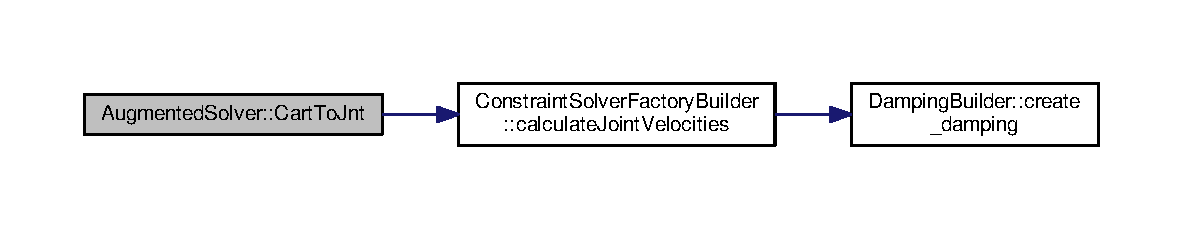
\includegraphics[width=350pt]{classAugmentedSolver_a9e0bf7d41497a64341b113b91c2c2011_cgraph}
\end{center}
\end{figure}




The documentation for this class was generated from the following files\-:\begin{DoxyCompactItemize}
\item 
/home/fxm-\/cm/catkin\-\_\-ws/src/cob\-\_\-control/cob\-\_\-twist\-\_\-controller/include/cob\-\_\-twist\-\_\-controller/\hyperlink{augmented__solver_8h}{augmented\-\_\-solver.\-h}\item 
/home/fxm-\/cm/catkin\-\_\-ws/src/cob\-\_\-control/cob\-\_\-twist\-\_\-controller/src/\hyperlink{augmented__solver_8cpp}{augmented\-\_\-solver.\-cpp}\end{DoxyCompactItemize}

\hypertarget{structAugmentedSolverParams}{\section{Augmented\-Solver\-Params Struct Reference}
\label{structAugmentedSolverParams}\index{Augmented\-Solver\-Params@{Augmented\-Solver\-Params}}
}
\subsection*{Public Attributes}
\begin{DoxyCompactItemize}
\item 
\hypertarget{structAugmentedSolverParams_a549501781701c0cf231c6b1313ebd9b5}{Damping\-Method\-Types {\bfseries damping\-\_\-method}}\label{structAugmentedSolverParams_a549501781701c0cf231c6b1313ebd9b5}

\item 
\hypertarget{structAugmentedSolverParams_ad7bcb8bbe49c08c976793e334083f9a6}{Contraint\-Types {\bfseries constraint}}\label{structAugmentedSolverParams_ad7bcb8bbe49c08c976793e334083f9a6}

\item 
\hypertarget{structAugmentedSolverParams_a299dbe15f6695d6d5221a490fea3c188}{double {\bfseries eps}}\label{structAugmentedSolverParams_a299dbe15f6695d6d5221a490fea3c188}

\item 
\hypertarget{structAugmentedSolverParams_a5167aa2d98246f3e6a5df19fcf4a6f02}{double {\bfseries damping\-\_\-factor}}\label{structAugmentedSolverParams_a5167aa2d98246f3e6a5df19fcf4a6f02}

\item 
\hypertarget{structAugmentedSolverParams_a7a7a045f0a42c198734c807209e420e4}{double {\bfseries lambda0}}\label{structAugmentedSolverParams_a7a7a045f0a42c198734c807209e420e4}

\item 
\hypertarget{structAugmentedSolverParams_a3b67245bd57d82a1343b2f2951ff6f28}{double {\bfseries wt}}\label{structAugmentedSolverParams_a3b67245bd57d82a1343b2f2951ff6f28}

\item 
\hypertarget{structAugmentedSolverParams_abe75c00241ca51f186376bfe0aa0bcd6}{bool {\bfseries base\-\_\-compensation}}\label{structAugmentedSolverParams_abe75c00241ca51f186376bfe0aa0bcd6}

\item 
\hypertarget{structAugmentedSolverParams_aa61616ab3b62fc41eacc414c33f8fb89}{bool {\bfseries base\-\_\-active}}\label{structAugmentedSolverParams_aa61616ab3b62fc41eacc414c33f8fb89}

\item 
\hypertarget{structAugmentedSolverParams_a7823582a731e8423a279db497a1a69d0}{double {\bfseries base\-\_\-ratio}}\label{structAugmentedSolverParams_a7823582a731e8423a279db497a1a69d0}

\item 
\hypertarget{structAugmentedSolverParams_a0755a09eb3ba40b0b97d4d41118b9e3b}{std\-::vector$<$ double $>$ {\bfseries limits\-\_\-max}}\label{structAugmentedSolverParams_a0755a09eb3ba40b0b97d4d41118b9e3b}

\item 
\hypertarget{structAugmentedSolverParams_a9b496c197c766e9cc398edf0deb429c2}{std\-::vector$<$ double $>$ {\bfseries limits\-\_\-min}}\label{structAugmentedSolverParams_a9b496c197c766e9cc398edf0deb429c2}

\end{DoxyCompactItemize}


The documentation for this struct was generated from the following file\-:\begin{DoxyCompactItemize}
\item 
/home/fxm-\/cm/catkin\-\_\-ws/src/cob\-\_\-control/cob\-\_\-twist\-\_\-controller/include/cob\-\_\-twist\-\_\-controller/\hyperlink{augmented__solver__data__types_8h}{augmented\-\_\-solver\-\_\-data\-\_\-types.\-h}\end{DoxyCompactItemize}

\hypertarget{classCobTwistController}{\section{Cob\-Twist\-Controller Class Reference}
\label{classCobTwistController}\index{Cob\-Twist\-Controller@{Cob\-Twist\-Controller}}
}
\subsection*{Public Member Functions}
\begin{DoxyCompactItemize}
\item 
bool \hyperlink{classCobTwistController_a9090539c07c0bfaef7d3e9c636cd1227}{initialize} ()
\item 
\hypertarget{classCobTwistController_a1aa93e5ae864cd5dba15f7f05069bb83}{void {\bfseries run} ()}\label{classCobTwistController_a1aa93e5ae864cd5dba15f7f05069bb83}

\item 
\hypertarget{classCobTwistController_a64f00b4e38aaa997b54c8c7cf2d2e56a}{void {\bfseries reconfigure\-\_\-callback} (cob\-\_\-twist\-\_\-controller\-::\-Twist\-Controller\-Config \&config, uint32\-\_\-t level)}\label{classCobTwistController_a64f00b4e38aaa997b54c8c7cf2d2e56a}

\item 
\hypertarget{classCobTwistController_a96e485efeff236806d5ce5ff163920cb}{void {\bfseries jointstate\-\_\-cb} (const sensor\-\_\-msgs\-::\-Joint\-State\-::\-Const\-Ptr \&msg)}\label{classCobTwistController_a96e485efeff236806d5ce5ff163920cb}

\item 
\hypertarget{classCobTwistController_af0cec45004d2902486cd54645fc29ca3}{void {\bfseries odometry\-\_\-cb} (const nav\-\_\-msgs\-::\-Odometry\-::\-Const\-Ptr \&msg)}\label{classCobTwistController_af0cec45004d2902486cd54645fc29ca3}

\item 
\hypertarget{classCobTwistController_a92c9f22fcbf87555371729c19ae87f91}{void \hyperlink{classCobTwistController_a92c9f22fcbf87555371729c19ae87f91}{twist\-\_\-cb} (const geometry\-\_\-msgs\-::\-Twist\-::\-Const\-Ptr \&msg)}\label{classCobTwistController_a92c9f22fcbf87555371729c19ae87f91}

\begin{DoxyCompactList}\small\item\em Orientation of twist\-\_\-msg is with respect to chain\-\_\-base coordinate system. \end{DoxyCompactList}\item 
\hypertarget{classCobTwistController_a7007a6628741fdbd97c840aedeb73617}{void {\bfseries base\-\_\-twist\-\_\-cb} (const geometry\-\_\-msgs\-::\-Twist\-::\-Const\-Ptr \&msg)}\label{classCobTwistController_a7007a6628741fdbd97c840aedeb73617}

\item 
\hypertarget{classCobTwistController_a5b769ea386acb685f2c553d09b6c2636}{void \hyperlink{classCobTwistController_a5b769ea386acb685f2c553d09b6c2636}{twist\-\_\-stamped\-\_\-cb} (const geometry\-\_\-msgs\-::\-Twist\-Stamped\-::\-Const\-Ptr \&msg)}\label{classCobTwistController_a5b769ea386acb685f2c553d09b6c2636}

\begin{DoxyCompactList}\small\item\em Orientation of twist\-\_\-stamped\-\_\-msg is with respect to coordinate system given in header.\-frame\-\_\-id. \end{DoxyCompactList}\item 
void \hyperlink{classCobTwistController_afe4ebcf7b22d5fb22c679e174fb61f25}{solve\-\_\-twist} (K\-D\-L\-::\-Twist twist)
\begin{DoxyCompactList}\small\item\em Orientation of twist is with respect to chain\-\_\-base coordinate system. \end{DoxyCompactList}\item 
\hypertarget{classCobTwistController_a0d04426df5a09a421510f65fd2a46e9d}{void \hyperlink{classCobTwistController_a0d04426df5a09a421510f65fd2a46e9d}{show\-Marker} (int marker\-\_\-id, double red, double green, double blue, std\-::string ns, ros\-::\-Publisher pub, std\-::vector$<$ geometry\-\_\-msgs\-::\-Point $>$ \&pos\-\_\-v)}\label{classCobTwistController_a0d04426df5a09a421510f65fd2a46e9d}

\begin{DoxyCompactList}\small\item\em Debug. \end{DoxyCompactList}\item 
\hypertarget{classCobTwistController_a48ef3bf6fc622a82f7ea7bf2f7f90464}{void {\bfseries debug} ()}\label{classCobTwistController_a48ef3bf6fc622a82f7ea7bf2f7f90464}

\end{DoxyCompactItemize}
\subsection*{Public Attributes}
\begin{DoxyCompactItemize}
\item 
\hypertarget{classCobTwistController_a1475837c311c21829eff6295d090a4d5}{boost\-::recursive\-\_\-mutex {\bfseries reconfig\-\_\-mutex\-\_\-}}\label{classCobTwistController_a1475837c311c21829eff6295d090a4d5}

\item 
\hypertarget{classCobTwistController_aeddd744f215a7cc1b0a097755ee22e4a}{boost\-::shared\-\_\-ptr\\*
$<$ dynamic\-\_\-reconfigure\-::\-Server\\*
$<$ cob\-\_\-twist\-\_\-controller\-::\-Twist\-Controller\-Config $>$ $>$ {\bfseries reconfigure\-\_\-server\-\_\-}}\label{classCobTwistController_aeddd744f215a7cc1b0a097755ee22e4a}

\end{DoxyCompactItemize}


\subsection{Member Function Documentation}
\hypertarget{classCobTwistController_a9090539c07c0bfaef7d3e9c636cd1227}{\index{Cob\-Twist\-Controller@{Cob\-Twist\-Controller}!initialize@{initialize}}
\index{initialize@{initialize}!CobTwistController@{Cob\-Twist\-Controller}}
\subsubsection[{initialize}]{\setlength{\rightskip}{0pt plus 5cm}bool Cob\-Twist\-Controller\-::initialize (
\begin{DoxyParamCaption}
{}
\end{DoxyParamCaption}
)}}\label{classCobTwistController_a9090539c07c0bfaef7d3e9c636cd1227}
parse robot\-\_\-description and generate K\-D\-L chains

parse robot\-\_\-description and set velocity limits

initialize configuration control solver

Setting up dynamic\-\_\-reconfigure server for the \hyperlink{structAugmentedSolverParams}{Augmented\-Solver\-Params}

initialize variables and current joint values and velocities

give tf\-\_\-listener some time to fill tf-\/cache

initialize R\-O\-S interfaces

Debug 

Here is the call graph for this function\-:
\nopagebreak
\begin{figure}[H]
\begin{center}
\leavevmode
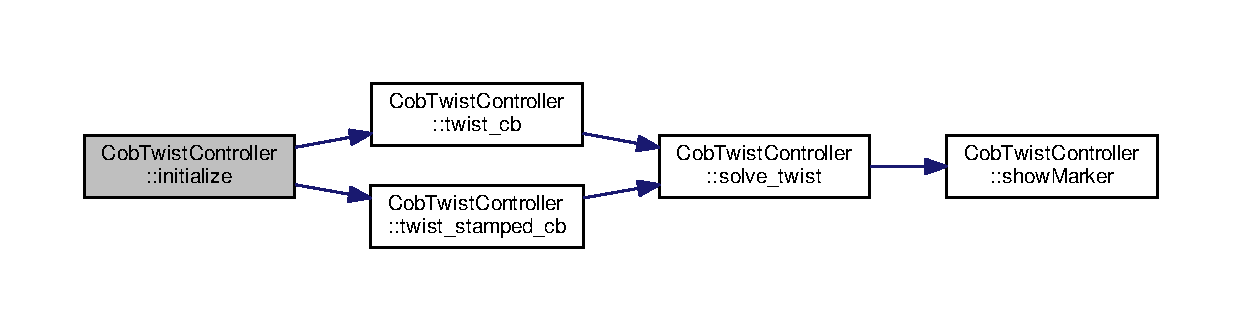
\includegraphics[width=350pt]{classCobTwistController_a9090539c07c0bfaef7d3e9c636cd1227_cgraph}
\end{center}
\end{figure}


\hypertarget{classCobTwistController_afe4ebcf7b22d5fb22c679e174fb61f25}{\index{Cob\-Twist\-Controller@{Cob\-Twist\-Controller}!solve\-\_\-twist@{solve\-\_\-twist}}
\index{solve\-\_\-twist@{solve\-\_\-twist}!CobTwistController@{Cob\-Twist\-Controller}}
\subsubsection[{solve\-\_\-twist}]{\setlength{\rightskip}{0pt plus 5cm}void Cob\-Twist\-Controller\-::solve\-\_\-twist (
\begin{DoxyParamCaption}
\item[{K\-D\-L\-::\-Twist}]{twist}
\end{DoxyParamCaption}
)}}\label{classCobTwistController_afe4ebcf7b22d5fb22c679e174fb61f25}


Orientation of twist is with respect to chain\-\_\-base coordinate system. 

Base Velocities with respect to base\-\_\-link 

Here is the call graph for this function\-:
\nopagebreak
\begin{figure}[H]
\begin{center}
\leavevmode
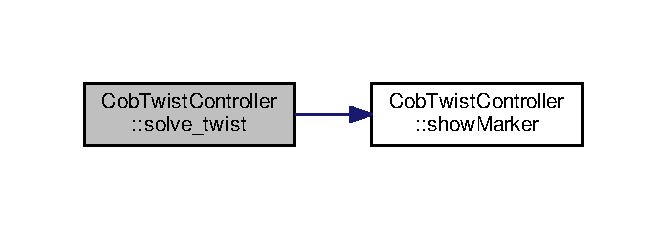
\includegraphics[width=320pt]{classCobTwistController_afe4ebcf7b22d5fb22c679e174fb61f25_cgraph}
\end{center}
\end{figure}




Here is the caller graph for this function\-:
\nopagebreak
\begin{figure}[H]
\begin{center}
\leavevmode
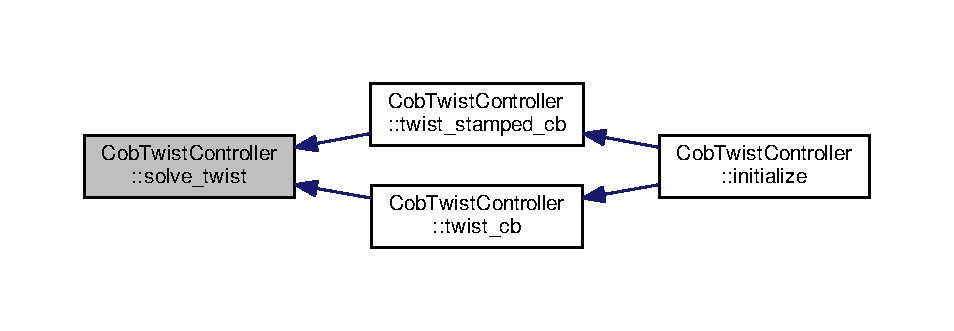
\includegraphics[width=350pt]{classCobTwistController_afe4ebcf7b22d5fb22c679e174fb61f25_icgraph}
\end{center}
\end{figure}




The documentation for this class was generated from the following files\-:\begin{DoxyCompactItemize}
\item 
/home/fxm-\/cm/catkin\-\_\-ws/src/cob\-\_\-control/cob\-\_\-twist\-\_\-controller/include/cob\-\_\-twist\-\_\-controller/\hyperlink{cob__twist__controller_8h}{cob\-\_\-twist\-\_\-controller.\-h}\item 
/home/fxm-\/cm/catkin\-\_\-ws/src/cob\-\_\-control/cob\-\_\-twist\-\_\-controller/src/\hyperlink{cob__twist__controller_8cpp}{cob\-\_\-twist\-\_\-controller.\-cpp}\end{DoxyCompactItemize}

\hypertarget{classConstraintSolver}{\section{Constraint\-Solver Class Reference}
\label{classConstraintSolver}\index{Constraint\-Solver@{Constraint\-Solver}}
}


Base class for solvers, defining interface methods.  




{\ttfamily \#include $<$constraint\-\_\-solver\-\_\-base.\-h$>$}



Inheritance diagram for Constraint\-Solver\-:
\nopagebreak
\begin{figure}[H]
\begin{center}
\leavevmode
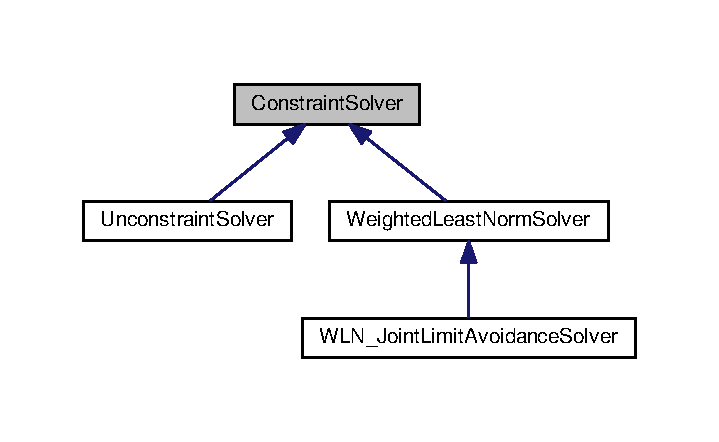
\includegraphics[width=345pt]{classConstraintSolver__inherit__graph}
\end{center}
\end{figure}


Collaboration diagram for Constraint\-Solver\-:
\nopagebreak
\begin{figure}[H]
\begin{center}
\leavevmode
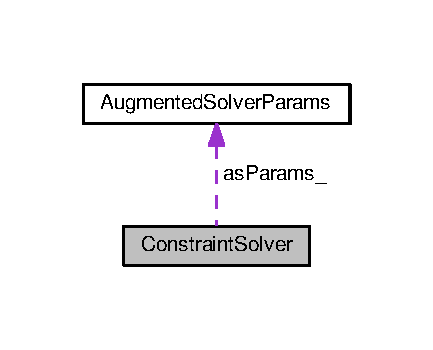
\includegraphics[width=208pt]{classConstraintSolver__coll__graph}
\end{center}
\end{figure}
\subsection*{Public Member Functions}
\begin{DoxyCompactItemize}
\item 
virtual Eigen\-::\-Matrix\-Xd \hyperlink{classConstraintSolver_a6208240cb2dc47fdd9adfc3a069408cd}{solve} (const Eigen\-::\-Vector\-Xd \&in\-Cart\-Velocities, const K\-D\-L\-::\-Jnt\-Array \&q, const K\-D\-L\-::\-Jnt\-Array \&last\-\_\-q\-\_\-dot) const =0
\item 
void \hyperlink{classConstraintSolver_aa28788d041bb495b0a2c94182e3a126f}{set\-Damping\-Factor} (double damping)
\end{DoxyCompactItemize}
\subsection*{Static Public Attributes}
\begin{DoxyCompactItemize}
\item 
\hypertarget{classConstraintSolver_a0dfdb039dd2a0c8b464410068e3b2ffb}{static const double \hyperlink{classConstraintSolver_a0dfdb039dd2a0c8b464410068e3b2ffb}{D\-A\-M\-P\-I\-N\-G\-\_\-\-L\-I\-M\-I\-T} = 1.\-0e-\/9}\label{classConstraintSolver_a0dfdb039dd2a0c8b464410068e3b2ffb}

\begin{DoxyCompactList}\small\item\em const. value for zero comparison with damping factor \end{DoxyCompactList}\end{DoxyCompactItemize}
\subsection*{Protected Member Functions}
\begin{DoxyCompactItemize}
\item 
\hypertarget{classConstraintSolver_adcb585a5c7f9e1c1d6fa1512e14a3213}{{\bfseries Constraint\-Solver} (\hyperlink{structAugmentedSolverParams}{Augmented\-Solver\-Params} \&as\-Params, Matrix6\-Xd \&jacobian\-Data)}\label{classConstraintSolver_adcb585a5c7f9e1c1d6fa1512e14a3213}

\item 
Eigen\-::\-Matrix\-Xd \hyperlink{classConstraintSolver_a015784de5861c9320991a3fd3523f232}{calculate\-Pinv\-Jacobian\-By\-S\-V\-D} (Eigen\-::\-Jacobi\-S\-V\-D$<$ Eigen\-::\-Matrix\-Xd $>$ svd) const 
\end{DoxyCompactItemize}
\subsection*{Protected Attributes}
\begin{DoxyCompactItemize}
\item 
\hypertarget{classConstraintSolver_ab0d5f3ad9e40ebe198a7fbf52ad93f60}{const \hyperlink{structAugmentedSolverParams}{Augmented\-Solver\-Params} \& \hyperlink{classConstraintSolver_ab0d5f3ad9e40ebe198a7fbf52ad93f60}{as\-Params\-\_\-}}\label{classConstraintSolver_ab0d5f3ad9e40ebe198a7fbf52ad93f60}

\begin{DoxyCompactList}\small\item\em References the augmented solver parameters. \end{DoxyCompactList}\item 
\hypertarget{classConstraintSolver_a7c926205c0aed8f7c6d6390a4b84a52d}{const Matrix6\-Xd \& \hyperlink{classConstraintSolver_a7c926205c0aed8f7c6d6390a4b84a52d}{jacobian\-Data\-\_\-}}\label{classConstraintSolver_a7c926205c0aed8f7c6d6390a4b84a52d}

\begin{DoxyCompactList}\small\item\em References the current Jacobian (matrix data only). \end{DoxyCompactList}\item 
\hypertarget{classConstraintSolver_a38e253500733cab242cfe8462963e2e7}{double \hyperlink{classConstraintSolver_a38e253500733cab242cfe8462963e2e7}{damping\-Factor\-\_\-}}\label{classConstraintSolver_a38e253500733cab242cfe8462963e2e7}

\begin{DoxyCompactList}\small\item\em The currently set damping factor. \end{DoxyCompactList}\end{DoxyCompactItemize}


\subsection{Detailed Description}
Base class for solvers, defining interface methods. 

\subsection{Member Function Documentation}
\hypertarget{classConstraintSolver_a015784de5861c9320991a3fd3523f232}{\index{Constraint\-Solver@{Constraint\-Solver}!calculate\-Pinv\-Jacobian\-By\-S\-V\-D@{calculate\-Pinv\-Jacobian\-By\-S\-V\-D}}
\index{calculate\-Pinv\-Jacobian\-By\-S\-V\-D@{calculate\-Pinv\-Jacobian\-By\-S\-V\-D}!ConstraintSolver@{Constraint\-Solver}}
\subsubsection[{calculate\-Pinv\-Jacobian\-By\-S\-V\-D}]{\setlength{\rightskip}{0pt plus 5cm}Eigen\-::\-Matrix\-Xd Constraint\-Solver\-::calculate\-Pinv\-Jacobian\-By\-S\-V\-D (
\begin{DoxyParamCaption}
\item[{Eigen\-::\-Jacobi\-S\-V\-D$<$ Eigen\-::\-Matrix\-Xd $>$}]{svd}
\end{DoxyParamCaption}
) const\hspace{0.3cm}{\ttfamily [protected]}}}\label{classConstraintSolver_a015784de5861c9320991a3fd3523f232}
Base method for calculation of the pseudoinverse Jacobian by using S\-V\-D. 
\begin{DoxyParams}{Parameters}
{\em svd} & The singular value decomposition object of a Jacobian. \\
\hline
\end{DoxyParams}
\begin{DoxyReturn}{Returns}
A pseudoinverse Jacobian
\end{DoxyReturn}
Calculates the pseudoinverse of a Jacobian by using S\-V\-D. Truncation is active always. Means if calculated (damped) singular value is $<$ than E\-P\-S than truncate the singular value to 0.\-0. Damping is active in case of $>$ than static const D\-A\-M\-P\-I\-N\-G\-\_\-\-L\-I\-M\-T, else it is assumed that no damping is active. 

Here is the caller graph for this function\-:
\nopagebreak
\begin{figure}[H]
\begin{center}
\leavevmode
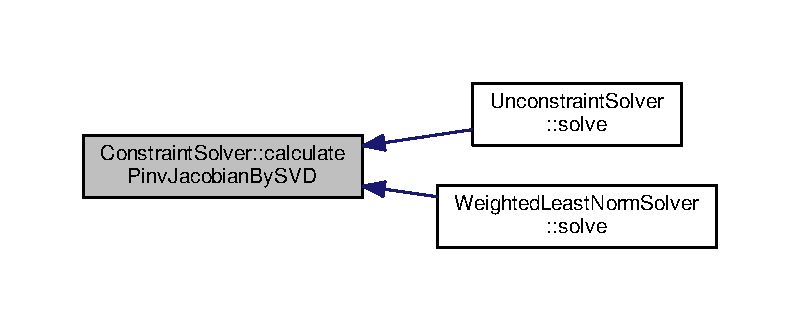
\includegraphics[width=350pt]{classConstraintSolver_a015784de5861c9320991a3fd3523f232_icgraph}
\end{center}
\end{figure}


\hypertarget{classConstraintSolver_aa28788d041bb495b0a2c94182e3a126f}{\index{Constraint\-Solver@{Constraint\-Solver}!set\-Damping\-Factor@{set\-Damping\-Factor}}
\index{set\-Damping\-Factor@{set\-Damping\-Factor}!ConstraintSolver@{Constraint\-Solver}}
\subsubsection[{set\-Damping\-Factor}]{\setlength{\rightskip}{0pt plus 5cm}void Constraint\-Solver\-::set\-Damping\-Factor (
\begin{DoxyParamCaption}
\item[{double}]{damping}
\end{DoxyParamCaption}
)\hspace{0.3cm}{\ttfamily [inline]}}}\label{classConstraintSolver_aa28788d041bb495b0a2c94182e3a126f}
Inline method to set the damping factor 
\begin{DoxyParams}{Parameters}
{\em damping} & The new damping factor \\
\hline
\end{DoxyParams}
\hypertarget{classConstraintSolver_a6208240cb2dc47fdd9adfc3a069408cd}{\index{Constraint\-Solver@{Constraint\-Solver}!solve@{solve}}
\index{solve@{solve}!ConstraintSolver@{Constraint\-Solver}}
\subsubsection[{solve}]{\setlength{\rightskip}{0pt plus 5cm}virtual Eigen\-::\-Matrix\-Xd Constraint\-Solver\-::solve (
\begin{DoxyParamCaption}
\item[{const Eigen\-::\-Vector\-Xd \&}]{in\-Cart\-Velocities, }
\item[{const K\-D\-L\-::\-Jnt\-Array \&}]{q, }
\item[{const K\-D\-L\-::\-Jnt\-Array \&}]{last\-\_\-q\-\_\-dot}
\end{DoxyParamCaption}
) const\hspace{0.3cm}{\ttfamily [pure virtual]}}}\label{classConstraintSolver_a6208240cb2dc47fdd9adfc3a069408cd}
The interface method to solve the inverse kinematics problem. Has to be implemented in inherited classes. 
\begin{DoxyParams}{Parameters}
{\em in\-Cart\-Velocities} & The input velocities vector (in cartesian space). \\
\hline
{\em q} & The current joint positions. \\
\hline
{\em last\-\_\-q\-\_\-dot} & The last joint velocities. \\
\hline
\end{DoxyParams}
\begin{DoxyReturn}{Returns}
The calculated new joint velocities. 
\end{DoxyReturn}


Implemented in \hyperlink{classWeightedLeastNormSolver_a0868fb81e9e75999037d96b4a6407ce7}{Weighted\-Least\-Norm\-Solver}, and \hyperlink{classUnconstraintSolver_a72e63efba891d2a55f4c95746b8d7b33}{Unconstraint\-Solver}.



The documentation for this class was generated from the following files\-:\begin{DoxyCompactItemize}
\item 
/home/fxm-\/cm/catkin\-\_\-ws/src/cob\-\_\-control/cob\-\_\-twist\-\_\-controller/include/cob\-\_\-twist\-\_\-controller/constraint\-\_\-solvers/solvers/\hyperlink{constraint__solver__base_8h}{constraint\-\_\-solver\-\_\-base.\-h}\item 
/home/fxm-\/cm/catkin\-\_\-ws/src/cob\-\_\-control/cob\-\_\-twist\-\_\-controller/src/constraint\-\_\-solvers/solvers/\hyperlink{constraint__solver__base_8cpp}{constraint\-\_\-solver\-\_\-base.\-cpp}\end{DoxyCompactItemize}

\hypertarget{classConstraintSolverFactoryBuilder}{\section{Constraint\-Solver\-Factory\-Builder Class Reference}
\label{classConstraintSolverFactoryBuilder}\index{Constraint\-Solver\-Factory\-Builder@{Constraint\-Solver\-Factory\-Builder}}
}


Static class providing a single method for creation of damping method, solver and starting the solving of the I\-K problem.  




{\ttfamily \#include $<$constraint\-\_\-solver\-\_\-factory\-\_\-builder.\-h$>$}

\subsection*{Static Public Member Functions}
\begin{DoxyCompactItemize}
\item 
static int8\-\_\-t \hyperlink{classConstraintSolverFactoryBuilder_a1d2eb736030aeea9156a20031d14e48a}{calculate\-Joint\-Velocities} (\hyperlink{structAugmentedSolverParams}{Augmented\-Solver\-Params} \&as\-Params, Matrix6\-Xd \&jacobian\-Data, const Eigen\-::\-Vector\-Xd \&in\-Cart\-Velocities, const K\-D\-L\-::\-Jnt\-Array \&q, const K\-D\-L\-::\-Jnt\-Array \&last\-\_\-q\-\_\-dot, Eigen\-::\-Matrix\-Xd \&out\-Jnt\-Velocities)
\end{DoxyCompactItemize}


\subsection{Detailed Description}
Static class providing a single method for creation of damping method, solver and starting the solving of the I\-K problem. 

\subsection{Member Function Documentation}
\hypertarget{classConstraintSolverFactoryBuilder_a1d2eb736030aeea9156a20031d14e48a}{\index{Constraint\-Solver\-Factory\-Builder@{Constraint\-Solver\-Factory\-Builder}!calculate\-Joint\-Velocities@{calculate\-Joint\-Velocities}}
\index{calculate\-Joint\-Velocities@{calculate\-Joint\-Velocities}!ConstraintSolverFactoryBuilder@{Constraint\-Solver\-Factory\-Builder}}
\subsubsection[{calculate\-Joint\-Velocities}]{\setlength{\rightskip}{0pt plus 5cm}int8\-\_\-t Constraint\-Solver\-Factory\-Builder\-::calculate\-Joint\-Velocities (
\begin{DoxyParamCaption}
\item[{{\bf Augmented\-Solver\-Params} \&}]{as\-Params, }
\item[{Matrix6\-Xd \&}]{jacobian\-Data, }
\item[{const Eigen\-::\-Vector\-Xd \&}]{in\-Cart\-Velocities, }
\item[{const K\-D\-L\-::\-Jnt\-Array \&}]{q, }
\item[{const K\-D\-L\-::\-Jnt\-Array \&}]{last\-\_\-q\-\_\-dot, }
\item[{Eigen\-::\-Matrix\-Xd \&}]{out\-Jnt\-Velocities}
\end{DoxyParamCaption}
)\hspace{0.3cm}{\ttfamily [static]}}}\label{classConstraintSolverFactoryBuilder_a1d2eb736030aeea9156a20031d14e48a}
Calculation of new joint velocities according to current joint positions and cartesian velocities. 
\begin{DoxyParams}{Parameters}
{\em as\-Params} & References the augmented solver parameters. \\
\hline
{\em jacobian\-Data} & References the current Jacobian (matrix data only). \\
\hline
{\em in\-Cart\-Velocities} & The input velocities vector (in cartesian space). \\
\hline
{\em q} & The current joint positions. \\
\hline
{\em last\-\_\-q\-\_\-dot} & The last joint velocities. \\
\hline
{\em out\-Jnt\-Velocities} & The calculated joint velocities as output reference. \\
\hline
\end{DoxyParams}
\begin{DoxyReturn}{Returns}
The calculated new joint velocities in (m x 1)-\/\-Matrix.
\end{DoxyReturn}
Out of the parameters generates a damping method (e.\-g. constant or manipulability) and calculates the damping factor. Dependent on J\-L\-A active flag a Joint\-Limit\-Avoidance\-Solver or a \hyperlink{classUnconstraintSolver}{Unconstraint\-Solver} is generated to solve the I\-K problem. The objects are generated for each solve-\/request. After calculation the objects are deleted. 

Here is the call graph for this function\-:
\nopagebreak
\begin{figure}[H]
\begin{center}
\leavevmode
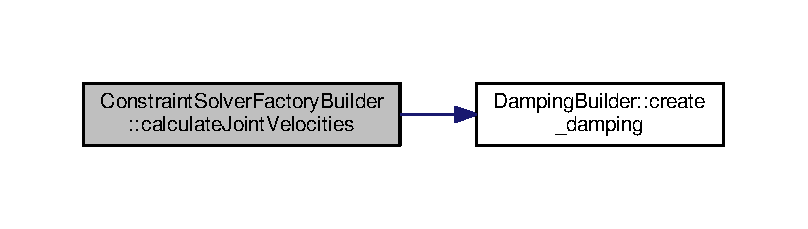
\includegraphics[width=350pt]{classConstraintSolverFactoryBuilder_a1d2eb736030aeea9156a20031d14e48a_cgraph}
\end{center}
\end{figure}




Here is the caller graph for this function\-:
\nopagebreak
\begin{figure}[H]
\begin{center}
\leavevmode
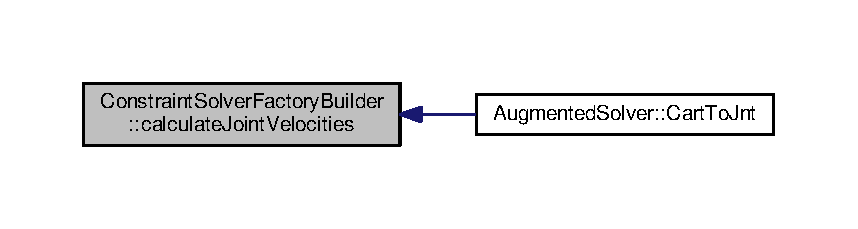
\includegraphics[width=350pt]{classConstraintSolverFactoryBuilder_a1d2eb736030aeea9156a20031d14e48a_icgraph}
\end{center}
\end{figure}




The documentation for this class was generated from the following files\-:\begin{DoxyCompactItemize}
\item 
/home/fxm-\/cm/catkin\-\_\-ws/src/cob\-\_\-control/cob\-\_\-twist\-\_\-controller/include/cob\-\_\-twist\-\_\-controller/constraint\-\_\-solvers/constraint\-\_\-solver\-\_\-factory\-\_\-builder.\-h\item 
/home/fxm-\/cm/catkin\-\_\-ws/src/cob\-\_\-control/cob\-\_\-twist\-\_\-controller/src/constraint\-\_\-solvers/constraint\-\_\-solver\-\_\-factory\-\_\-builder.\-cpp\end{DoxyCompactItemize}

\hypertarget{classDampingBase}{\section{Damping\-Base Class Reference}
\label{classDampingBase}\index{Damping\-Base@{Damping\-Base}}
}


Base class for solvers, defining interface methods.  




{\ttfamily \#include $<$damping\-\_\-base.\-h$>$}



Inheritance diagram for Damping\-Base\-:
\nopagebreak
\begin{figure}[H]
\begin{center}
\leavevmode
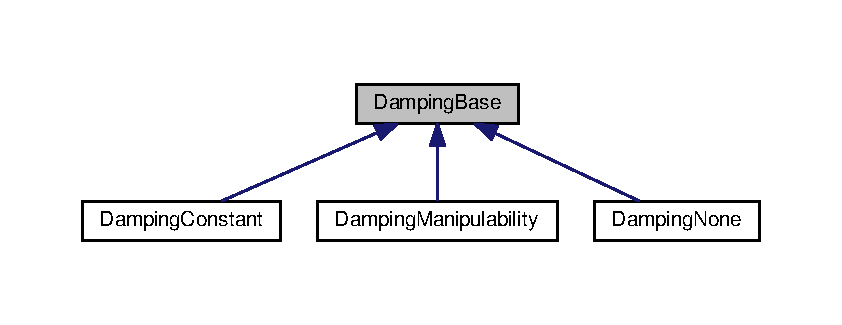
\includegraphics[width=350pt]{classDampingBase__inherit__graph}
\end{center}
\end{figure}


Collaboration diagram for Damping\-Base\-:
\nopagebreak
\begin{figure}[H]
\begin{center}
\leavevmode
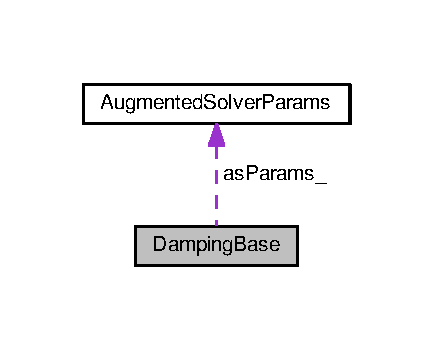
\includegraphics[width=208pt]{classDampingBase__coll__graph}
\end{center}
\end{figure}
\subsection*{Public Member Functions}
\begin{DoxyCompactItemize}
\item 
\hypertarget{classDampingBase_a0ff0d06272159afec03cf291d79d88e6}{virtual double {\bfseries get\-\_\-damping\-\_\-factor} () const =0}\label{classDampingBase_a0ff0d06272159afec03cf291d79d88e6}

\end{DoxyCompactItemize}
\subsection*{Protected Member Functions}
\begin{DoxyCompactItemize}
\item 
\hypertarget{classDampingBase_a896950a881805c92878f7888e8d5362a}{{\bfseries Damping\-Base} (\hyperlink{structAugmentedSolverParams}{Augmented\-Solver\-Params} \&as\-Params, Matrix6\-Xd \&jacobian\-Data)}\label{classDampingBase_a896950a881805c92878f7888e8d5362a}

\end{DoxyCompactItemize}
\subsection*{Protected Attributes}
\begin{DoxyCompactItemize}
\item 
\hypertarget{classDampingBase_af7a090118a27826f63f51e3b850104e1}{const \hyperlink{structAugmentedSolverParams}{Augmented\-Solver\-Params} \& {\bfseries as\-Params\-\_\-}}\label{classDampingBase_af7a090118a27826f63f51e3b850104e1}

\item 
\hypertarget{classDampingBase_ad5194f9da74dae956b2ce5daff659ce3}{const Matrix6\-Xd \& {\bfseries jacobian\-Data\-\_\-}}\label{classDampingBase_ad5194f9da74dae956b2ce5daff659ce3}

\end{DoxyCompactItemize}


\subsection{Detailed Description}
Base class for solvers, defining interface methods. 

The documentation for this class was generated from the following files\-:\begin{DoxyCompactItemize}
\item 
/home/fxm-\/cm/catkin\-\_\-ws/src/cob\-\_\-control/cob\-\_\-twist\-\_\-controller/include/cob\-\_\-twist\-\_\-controller/damping\-\_\-methods/\hyperlink{damping__base_8h}{damping\-\_\-base.\-h}\item 
/home/fxm-\/cm/catkin\-\_\-ws/src/cob\-\_\-control/cob\-\_\-twist\-\_\-controller/src/damping\-\_\-methods/\hyperlink{damping__base_8cpp}{damping\-\_\-base.\-cpp}\end{DoxyCompactItemize}

\hypertarget{classDampingBuilder}{\section{Damping\-Builder Class Reference}
\label{classDampingBuilder}\index{Damping\-Builder@{Damping\-Builder}}
}


Class providing a static method to create damping method objects.  




{\ttfamily \#include $<$damping.\-h$>$}

\subsection*{Static Public Member Functions}
\begin{DoxyCompactItemize}
\item 
static \hyperlink{classDampingBase}{Damping\-Base} $\ast$ \hyperlink{classDampingBuilder_a15f58f4523f13e73897fc6114c322fee}{create\-\_\-damping} (\hyperlink{structAugmentedSolverParams}{Augmented\-Solver\-Params} \&augmented\-Solver\-Params, Matrix6\-Xd \&jacobian\-Data)
\end{DoxyCompactItemize}


\subsection{Detailed Description}
Class providing a static method to create damping method objects. 

\subsection{Member Function Documentation}
\hypertarget{classDampingBuilder_a15f58f4523f13e73897fc6114c322fee}{\index{Damping\-Builder@{Damping\-Builder}!create\-\_\-damping@{create\-\_\-damping}}
\index{create\-\_\-damping@{create\-\_\-damping}!DampingBuilder@{Damping\-Builder}}
\subsubsection[{create\-\_\-damping}]{\setlength{\rightskip}{0pt plus 5cm}{\bf Damping\-Base} $\ast$ Damping\-Builder\-::create\-\_\-damping (
\begin{DoxyParamCaption}
\item[{{\bf Augmented\-Solver\-Params} \&}]{augmented\-Solver\-Params, }
\item[{Matrix6\-Xd \&}]{jacobian\-Data}
\end{DoxyParamCaption}
)\hspace{0.3cm}{\ttfamily [static]}}}\label{classDampingBuilder_a15f58f4523f13e73897fc6114c322fee}
Static builder method to create damping methods dependent on parameterization. 

Here is the caller graph for this function\-:
\nopagebreak
\begin{figure}[H]
\begin{center}
\leavevmode
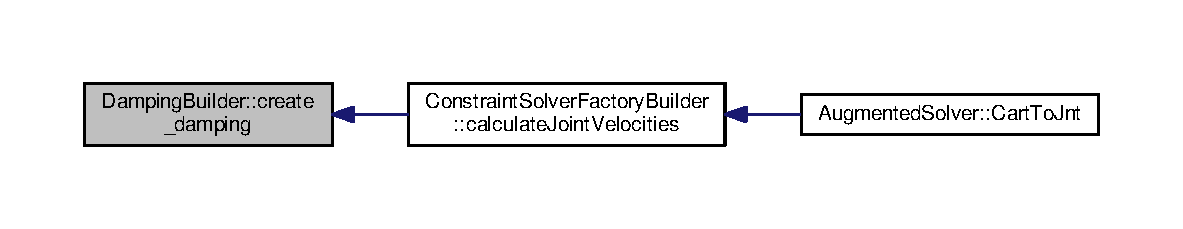
\includegraphics[width=350pt]{classDampingBuilder_a15f58f4523f13e73897fc6114c322fee_icgraph}
\end{center}
\end{figure}




The documentation for this class was generated from the following files\-:\begin{DoxyCompactItemize}
\item 
/home/fxm-\/cm/catkin\-\_\-ws/src/cob\-\_\-control/cob\-\_\-twist\-\_\-controller/include/cob\-\_\-twist\-\_\-controller/damping\-\_\-methods/\hyperlink{damping_8h}{damping.\-h}\item 
/home/fxm-\/cm/catkin\-\_\-ws/src/cob\-\_\-control/cob\-\_\-twist\-\_\-controller/src/damping\-\_\-methods/\hyperlink{damping_8cpp}{damping.\-cpp}\end{DoxyCompactItemize}

\hypertarget{classDampingConstant}{\section{Damping\-Constant Class Reference}
\label{classDampingConstant}\index{Damping\-Constant@{Damping\-Constant}}
}


Class implementing a method to return the constant factor.  




{\ttfamily \#include $<$damping.\-h$>$}



Inheritance diagram for Damping\-Constant\-:
\nopagebreak
\begin{figure}[H]
\begin{center}
\leavevmode
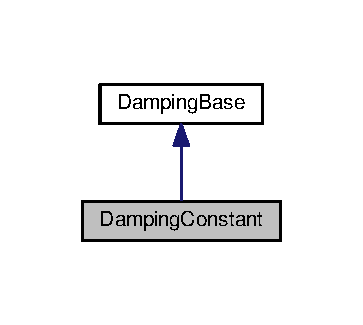
\includegraphics[width=174pt]{classDampingConstant__inherit__graph}
\end{center}
\end{figure}


Collaboration diagram for Damping\-Constant\-:
\nopagebreak
\begin{figure}[H]
\begin{center}
\leavevmode
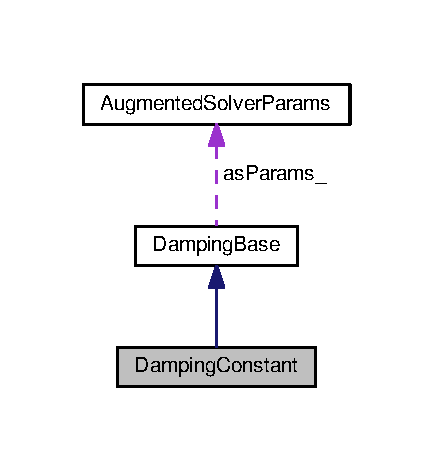
\includegraphics[width=208pt]{classDampingConstant__coll__graph}
\end{center}
\end{figure}
\subsection*{Public Member Functions}
\begin{DoxyCompactItemize}
\item 
\hypertarget{classDampingConstant_a14b052539cb1d3d1b8af399f1a2b7f00}{{\bfseries Damping\-Constant} (\hyperlink{structAugmentedSolverParams}{Augmented\-Solver\-Params} \&as\-Params, Matrix6\-Xd \&jacobian\-Data)}\label{classDampingConstant_a14b052539cb1d3d1b8af399f1a2b7f00}

\item 
virtual double \hyperlink{classDampingConstant_a3767d946f2b36dc221671e50a93c3dd7}{get\-\_\-damping\-\_\-factor} () const 
\end{DoxyCompactItemize}
\subsection*{Additional Inherited Members}


\subsection{Detailed Description}
Class implementing a method to return the constant factor. 

\subsection{Member Function Documentation}
\hypertarget{classDampingConstant_a3767d946f2b36dc221671e50a93c3dd7}{\index{Damping\-Constant@{Damping\-Constant}!get\-\_\-damping\-\_\-factor@{get\-\_\-damping\-\_\-factor}}
\index{get\-\_\-damping\-\_\-factor@{get\-\_\-damping\-\_\-factor}!DampingConstant@{Damping\-Constant}}
\subsubsection[{get\-\_\-damping\-\_\-factor}]{\setlength{\rightskip}{0pt plus 5cm}double Damping\-Constant\-::get\-\_\-damping\-\_\-factor (
\begin{DoxyParamCaption}
{}
\end{DoxyParamCaption}
) const\hspace{0.3cm}{\ttfamily [inline]}, {\ttfamily [virtual]}}}\label{classDampingConstant_a3767d946f2b36dc221671e50a93c3dd7}
Method just returns the damping factor from ros parameter server. 

Implements \hyperlink{classDampingBase}{Damping\-Base}.



The documentation for this class was generated from the following files\-:\begin{DoxyCompactItemize}
\item 
/home/fxm-\/cm/catkin\-\_\-ws/src/cob\-\_\-control/cob\-\_\-twist\-\_\-controller/include/cob\-\_\-twist\-\_\-controller/damping\-\_\-methods/\hyperlink{damping_8h}{damping.\-h}\item 
/home/fxm-\/cm/catkin\-\_\-ws/src/cob\-\_\-control/cob\-\_\-twist\-\_\-controller/src/damping\-\_\-methods/\hyperlink{damping_8cpp}{damping.\-cpp}\end{DoxyCompactItemize}

\hypertarget{classDampingManipulability}{\section{Damping\-Manipulability Class Reference}
\label{classDampingManipulability}\index{Damping\-Manipulability@{Damping\-Manipulability}}
}


Class implementing a method to return a factor corresponding to the measure of manipulability.  




{\ttfamily \#include $<$damping.\-h$>$}



Inheritance diagram for Damping\-Manipulability\-:
\nopagebreak
\begin{figure}[H]
\begin{center}
\leavevmode
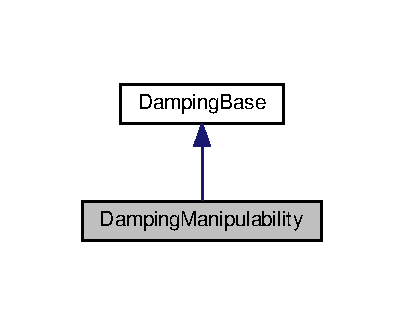
\includegraphics[width=194pt]{classDampingManipulability__inherit__graph}
\end{center}
\end{figure}


Collaboration diagram for Damping\-Manipulability\-:
\nopagebreak
\begin{figure}[H]
\begin{center}
\leavevmode
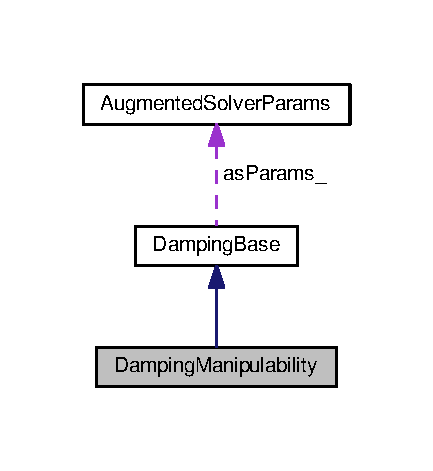
\includegraphics[width=208pt]{classDampingManipulability__coll__graph}
\end{center}
\end{figure}
\subsection*{Public Member Functions}
\begin{DoxyCompactItemize}
\item 
\hypertarget{classDampingManipulability_ab690b0a6cb3391e4eb1d83043b91d689}{{\bfseries Damping\-Manipulability} (\hyperlink{structAugmentedSolverParams}{Augmented\-Solver\-Params} \&as\-Params, Matrix6\-Xd \&jacobian\-Data)}\label{classDampingManipulability_ab690b0a6cb3391e4eb1d83043b91d689}

\item 
virtual double \hyperlink{classDampingManipulability_a3002c079481a0da5fd88c611000d25de}{get\-\_\-damping\-\_\-factor} () const 
\end{DoxyCompactItemize}
\subsection*{Additional Inherited Members}


\subsection{Detailed Description}
Class implementing a method to return a factor corresponding to the measure of manipulability. 

\subsection{Member Function Documentation}
\hypertarget{classDampingManipulability_a3002c079481a0da5fd88c611000d25de}{\index{Damping\-Manipulability@{Damping\-Manipulability}!get\-\_\-damping\-\_\-factor@{get\-\_\-damping\-\_\-factor}}
\index{get\-\_\-damping\-\_\-factor@{get\-\_\-damping\-\_\-factor}!DampingManipulability@{Damping\-Manipulability}}
\subsubsection[{get\-\_\-damping\-\_\-factor}]{\setlength{\rightskip}{0pt plus 5cm}double Damping\-Manipulability\-::get\-\_\-damping\-\_\-factor (
\begin{DoxyParamCaption}
{}
\end{DoxyParamCaption}
) const\hspace{0.3cm}{\ttfamily [virtual]}}}\label{classDampingManipulability_a3002c079481a0da5fd88c611000d25de}
Method returns the damping factor according to the manipulability measure. \mbox{[}Nakamura, \char`\"{}\-Advanced Robotics Redundancy and Optimization\char`\"{}, I\-S\-B\-N\-: 0-\/201-\/15198-\/7, Page 268\mbox{]} 

Implements \hyperlink{classDampingBase}{Damping\-Base}.



The documentation for this class was generated from the following files\-:\begin{DoxyCompactItemize}
\item 
/home/fxm-\/cm/catkin\-\_\-ws/src/cob\-\_\-control/cob\-\_\-twist\-\_\-controller/include/cob\-\_\-twist\-\_\-controller/damping\-\_\-methods/\hyperlink{damping_8h}{damping.\-h}\item 
/home/fxm-\/cm/catkin\-\_\-ws/src/cob\-\_\-control/cob\-\_\-twist\-\_\-controller/src/damping\-\_\-methods/\hyperlink{damping_8cpp}{damping.\-cpp}\end{DoxyCompactItemize}

\hypertarget{classDampingNone}{\section{Damping\-None Class Reference}
\label{classDampingNone}\index{Damping\-None@{Damping\-None}}
}


Class implementing a method to return the constant factor.  




{\ttfamily \#include $<$damping.\-h$>$}



Inheritance diagram for Damping\-None\-:
\nopagebreak
\begin{figure}[H]
\begin{center}
\leavevmode
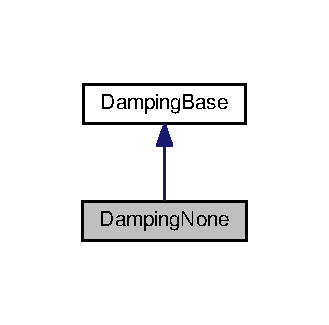
\includegraphics[width=158pt]{classDampingNone__inherit__graph}
\end{center}
\end{figure}


Collaboration diagram for Damping\-None\-:
\nopagebreak
\begin{figure}[H]
\begin{center}
\leavevmode
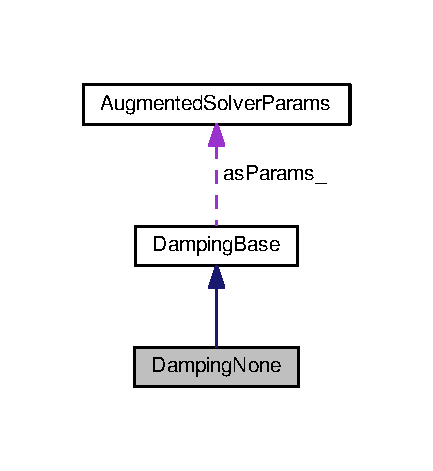
\includegraphics[width=208pt]{classDampingNone__coll__graph}
\end{center}
\end{figure}
\subsection*{Public Member Functions}
\begin{DoxyCompactItemize}
\item 
\hypertarget{classDampingNone_a11ea63a5d94981ddd494a35daaa251e7}{{\bfseries Damping\-None} (\hyperlink{structAugmentedSolverParams}{Augmented\-Solver\-Params} \&as\-Params, Matrix6\-Xd \&jacobian\-Data)}\label{classDampingNone_a11ea63a5d94981ddd494a35daaa251e7}

\item 
virtual double \hyperlink{classDampingNone_a9035956df3b8f0544557e836d3ecd7ab}{get\-\_\-damping\-\_\-factor} () const 
\end{DoxyCompactItemize}
\subsection*{Additional Inherited Members}


\subsection{Detailed Description}
Class implementing a method to return the constant factor. 

\subsection{Member Function Documentation}
\hypertarget{classDampingNone_a9035956df3b8f0544557e836d3ecd7ab}{\index{Damping\-None@{Damping\-None}!get\-\_\-damping\-\_\-factor@{get\-\_\-damping\-\_\-factor}}
\index{get\-\_\-damping\-\_\-factor@{get\-\_\-damping\-\_\-factor}!DampingNone@{Damping\-None}}
\subsubsection[{get\-\_\-damping\-\_\-factor}]{\setlength{\rightskip}{0pt plus 5cm}double Damping\-None\-::get\-\_\-damping\-\_\-factor (
\begin{DoxyParamCaption}
{}
\end{DoxyParamCaption}
) const\hspace{0.3cm}{\ttfamily [inline]}, {\ttfamily [virtual]}}}\label{classDampingNone_a9035956df3b8f0544557e836d3ecd7ab}
Method just returns the damping factor from ros parameter server. 

Implements \hyperlink{classDampingBase}{Damping\-Base}.



The documentation for this class was generated from the following files\-:\begin{DoxyCompactItemize}
\item 
/home/fxm-\/cm/catkin\-\_\-ws/src/cob\-\_\-control/cob\-\_\-twist\-\_\-controller/include/cob\-\_\-twist\-\_\-controller/damping\-\_\-methods/\hyperlink{damping_8h}{damping.\-h}\item 
/home/fxm-\/cm/catkin\-\_\-ws/src/cob\-\_\-control/cob\-\_\-twist\-\_\-controller/src/damping\-\_\-methods/\hyperlink{damping_8cpp}{damping.\-cpp}\end{DoxyCompactItemize}

\hypertarget{classISolverFactory}{\section{I\-Solver\-Factory Class Reference}
\label{classISolverFactory}\index{I\-Solver\-Factory@{I\-Solver\-Factory}}
}


Interface definition to support generic usage of the solver factory without specifying a typename in prior.  




{\ttfamily \#include $<$solver\-\_\-factory.\-h$>$}



Inheritance diagram for I\-Solver\-Factory\-:
\nopagebreak
\begin{figure}[H]
\begin{center}
\leavevmode
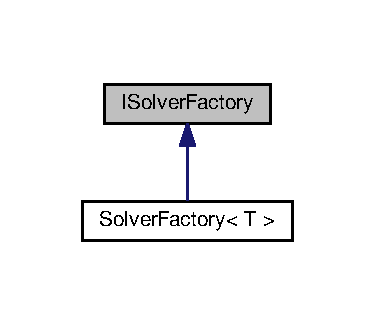
\includegraphics[width=180pt]{classISolverFactory__inherit__graph}
\end{center}
\end{figure}
\subsection*{Public Member Functions}
\begin{DoxyCompactItemize}
\item 
\hypertarget{classISolverFactory_a7b0cccec09597d71cf67da38d7bf6f5b}{virtual Eigen\-::\-Matrix\-Xd {\bfseries calculate\-Joint\-Velocities} (\hyperlink{structAugmentedSolverParams}{Augmented\-Solver\-Params} \&as\-Params, Matrix6\-Xd \&jacobian\-Data, const Eigen\-::\-Vector\-Xd \&in\-Cart\-Velocities, const K\-D\-L\-::\-Jnt\-Array \&q, const K\-D\-L\-::\-Jnt\-Array \&last\-\_\-q\-\_\-dot, double damping\-Factor) const =0}\label{classISolverFactory_a7b0cccec09597d71cf67da38d7bf6f5b}

\end{DoxyCompactItemize}


\subsection{Detailed Description}
Interface definition to support generic usage of the solver factory without specifying a typename in prior. 

The documentation for this class was generated from the following file\-:\begin{DoxyCompactItemize}
\item 
/home/fxm-\/cm/catkin\-\_\-ws/src/cob\-\_\-control/cob\-\_\-twist\-\_\-controller/include/cob\-\_\-twist\-\_\-controller/constraint\-\_\-solvers/factories/\hyperlink{solver__factory_8h}{solver\-\_\-factory.\-h}\end{DoxyCompactItemize}

\hypertarget{classLimiterAllJointPositions}{\section{Limiter\-All\-Joint\-Positions Class Reference}
\label{classLimiterAllJointPositions}\index{Limiter\-All\-Joint\-Positions@{Limiter\-All\-Joint\-Positions}}
}


Class for limiters, declaring the method to limit all joint positions.  




{\ttfamily \#include $<$limiter.\-h$>$}



Inheritance diagram for Limiter\-All\-Joint\-Positions\-:
\nopagebreak
\begin{figure}[H]
\begin{center}
\leavevmode
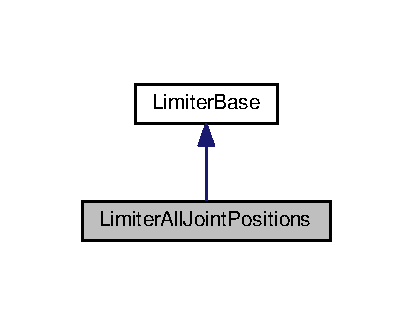
\includegraphics[width=198pt]{classLimiterAllJointPositions__inherit__graph}
\end{center}
\end{figure}


Collaboration diagram for Limiter\-All\-Joint\-Positions\-:
\nopagebreak
\begin{figure}[H]
\begin{center}
\leavevmode
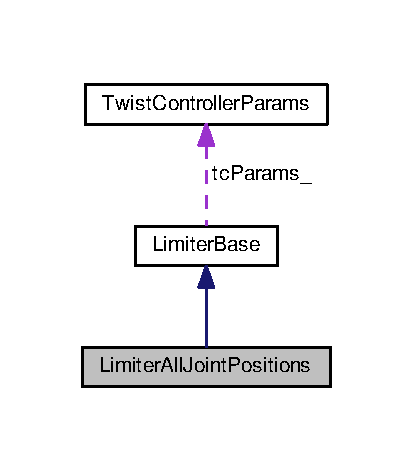
\includegraphics[width=198pt]{classLimiterAllJointPositions__coll__graph}
\end{center}
\end{figure}
\subsection*{Public Member Functions}
\begin{DoxyCompactItemize}
\item 
virtual K\-D\-L\-::\-Jnt\-Array \hyperlink{classLimiterAllJointPositions_af4dc11b0adfe3eea38d1291b09a2a693}{enforce\-Limits} (const K\-D\-L\-::\-Jnt\-Array \&q\-\_\-dot\-\_\-ik, const K\-D\-L\-::\-Jnt\-Array \&q) const 
\item 
\hypertarget{classLimiterAllJointPositions_a19ad99c1ca465381ec7b9c5264559513}{{\bfseries Limiter\-All\-Joint\-Positions} (const \hyperlink{structTwistControllerParams}{Twist\-Controller\-Params} \&tc\-Params, const K\-D\-L\-::\-Chain \&chain)}\label{classLimiterAllJointPositions_a19ad99c1ca465381ec7b9c5264559513}

\end{DoxyCompactItemize}
\subsection*{Additional Inherited Members}


\subsection{Detailed Description}
Class for limiters, declaring the method to limit all joint positions. 

\subsection{Member Function Documentation}
\hypertarget{classLimiterAllJointPositions_af4dc11b0adfe3eea38d1291b09a2a693}{\index{Limiter\-All\-Joint\-Positions@{Limiter\-All\-Joint\-Positions}!enforce\-Limits@{enforce\-Limits}}
\index{enforce\-Limits@{enforce\-Limits}!LimiterAllJointPositions@{Limiter\-All\-Joint\-Positions}}
\subsubsection[{enforce\-Limits}]{\setlength{\rightskip}{0pt plus 5cm}K\-D\-L\-::\-Jnt\-Array Limiter\-All\-Joint\-Positions\-::enforce\-Limits (
\begin{DoxyParamCaption}
\item[{const K\-D\-L\-::\-Jnt\-Array \&}]{q\-\_\-dot\-\_\-ik, }
\item[{const K\-D\-L\-::\-Jnt\-Array \&}]{q}
\end{DoxyParamCaption}
) const\hspace{0.3cm}{\ttfamily [virtual]}}}\label{classLimiterAllJointPositions_af4dc11b0adfe3eea38d1291b09a2a693}
Specific implementation of enforce\-Limits-\/method. See base class \hyperlink{classLimiterBase}{Limiter\-Base} for more details on params and returns.

Checks the positions of the joints whether the are in tolerance or not. If not the corresponding velocities vector is scaled. This function multiplies the velocities that result from the I\-K with a limits-\/dependent factor in case the joint positions violate the specified tolerance. The factor is calculated by using the cosine function to provide a smooth transition from 1 to zero. Factor is applied on all joint velocities (although only one joint has exceeded its limits), so that the direction of the desired twist is not changed. -\/$>$ Important for the Use-\/\-Case to follow a trajectory exactly! 

Implements \hyperlink{classLimiterBase_a1755edebc0cacfd79f945852ead8ae04}{Limiter\-Base}.



The documentation for this class was generated from the following files\-:\begin{DoxyCompactItemize}
\item 
/home/fxm-\/cm/catkin\-\_\-ws/src/cob\-\_\-control/cob\-\_\-twist\-\_\-controller/include/cob\-\_\-twist\-\_\-controller/limiters/\hyperlink{limiter_8h}{limiter.\-h}\item 
/home/fxm-\/cm/catkin\-\_\-ws/src/cob\-\_\-control/cob\-\_\-twist\-\_\-controller/src/limiters/\hyperlink{limiter_8cpp}{limiter.\-cpp}\end{DoxyCompactItemize}

\hypertarget{classLimiterAllJointVelocities}{\section{Limiter\-All\-Joint\-Velocities Class Reference}
\label{classLimiterAllJointVelocities}\index{Limiter\-All\-Joint\-Velocities@{Limiter\-All\-Joint\-Velocities}}
}


Class for joint velocity limiter (all scaled to keep direction), implementing interface methods.  




{\ttfamily \#include $<$limiter.\-h$>$}



Inheritance diagram for Limiter\-All\-Joint\-Velocities\-:
\nopagebreak
\begin{figure}[H]
\begin{center}
\leavevmode
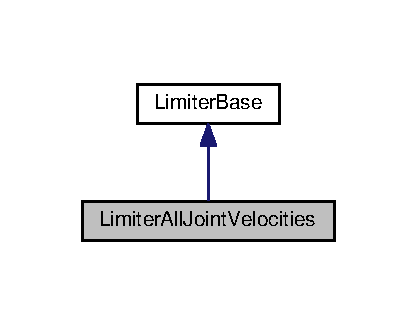
\includegraphics[width=200pt]{classLimiterAllJointVelocities__inherit__graph}
\end{center}
\end{figure}


Collaboration diagram for Limiter\-All\-Joint\-Velocities\-:
\nopagebreak
\begin{figure}[H]
\begin{center}
\leavevmode
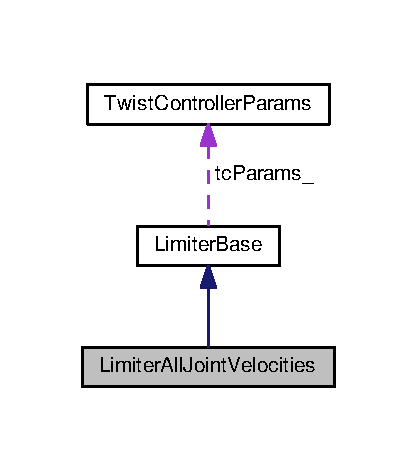
\includegraphics[width=200pt]{classLimiterAllJointVelocities__coll__graph}
\end{center}
\end{figure}
\subsection*{Public Member Functions}
\begin{DoxyCompactItemize}
\item 
virtual K\-D\-L\-::\-Jnt\-Array \hyperlink{classLimiterAllJointVelocities_aa068927c99f27d9616fe5bdd7fd7248d}{enforce\-Limits} (const K\-D\-L\-::\-Jnt\-Array \&q\-\_\-dot\-\_\-ik, const K\-D\-L\-::\-Jnt\-Array \&q) const 
\item 
\hypertarget{classLimiterAllJointVelocities_a623ed13f38a32d87cfaefa4b1e8be48c}{{\bfseries Limiter\-All\-Joint\-Velocities} (const \hyperlink{structTwistControllerParams}{Twist\-Controller\-Params} \&tc\-Params, const K\-D\-L\-::\-Chain \&chain)}\label{classLimiterAllJointVelocities_a623ed13f38a32d87cfaefa4b1e8be48c}

\end{DoxyCompactItemize}
\subsection*{Additional Inherited Members}


\subsection{Detailed Description}
Class for joint velocity limiter (all scaled to keep direction), implementing interface methods. 

\subsection{Member Function Documentation}
\hypertarget{classLimiterAllJointVelocities_aa068927c99f27d9616fe5bdd7fd7248d}{\index{Limiter\-All\-Joint\-Velocities@{Limiter\-All\-Joint\-Velocities}!enforce\-Limits@{enforce\-Limits}}
\index{enforce\-Limits@{enforce\-Limits}!LimiterAllJointVelocities@{Limiter\-All\-Joint\-Velocities}}
\subsubsection[{enforce\-Limits}]{\setlength{\rightskip}{0pt plus 5cm}K\-D\-L\-::\-Jnt\-Array Limiter\-All\-Joint\-Velocities\-::enforce\-Limits (
\begin{DoxyParamCaption}
\item[{const K\-D\-L\-::\-Jnt\-Array \&}]{q\-\_\-dot\-\_\-ik, }
\item[{const K\-D\-L\-::\-Jnt\-Array \&}]{q}
\end{DoxyParamCaption}
) const\hspace{0.3cm}{\ttfamily [virtual]}}}\label{classLimiterAllJointVelocities_aa068927c99f27d9616fe5bdd7fd7248d}
Specific implementation of enforce\-Limits-\/method. See base class \hyperlink{classLimiterBase}{Limiter\-Base} for more details on params and returns.

Enforce limits on all joint velocities to keep direction (former known as normalize\-\_\-velocities). Limits all velocities according to the limits\-\_\-vel vector if necessary. 

Implements \hyperlink{classLimiterBase_a1755edebc0cacfd79f945852ead8ae04}{Limiter\-Base}.



The documentation for this class was generated from the following files\-:\begin{DoxyCompactItemize}
\item 
/home/fxm-\/cm/catkin\-\_\-ws/src/cob\-\_\-control/cob\-\_\-twist\-\_\-controller/include/cob\-\_\-twist\-\_\-controller/limiters/\hyperlink{limiter_8h}{limiter.\-h}\item 
/home/fxm-\/cm/catkin\-\_\-ws/src/cob\-\_\-control/cob\-\_\-twist\-\_\-controller/src/limiters/\hyperlink{limiter_8cpp}{limiter.\-cpp}\end{DoxyCompactItemize}

\hypertarget{classLimiterBase}{\section{Limiter\-Base Class Reference}
\label{classLimiterBase}\index{Limiter\-Base@{Limiter\-Base}}
}


Base class for limiters, defining interface methods.  




{\ttfamily \#include $<$limiter\-\_\-base.\-h$>$}



Inheritance diagram for Limiter\-Base\-:
\nopagebreak
\begin{figure}[H]
\begin{center}
\leavevmode
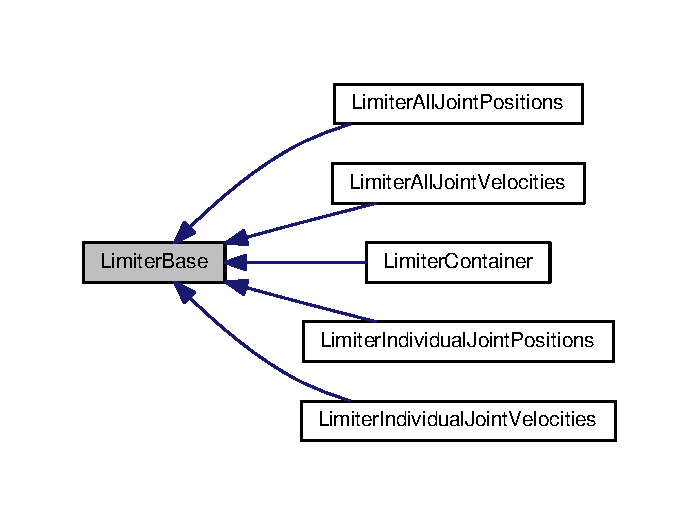
\includegraphics[width=336pt]{classLimiterBase__inherit__graph}
\end{center}
\end{figure}


Collaboration diagram for Limiter\-Base\-:
\nopagebreak
\begin{figure}[H]
\begin{center}
\leavevmode
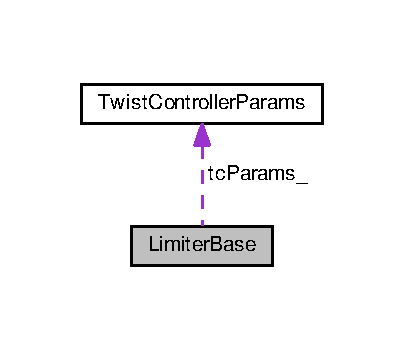
\includegraphics[width=194pt]{classLimiterBase__coll__graph}
\end{center}
\end{figure}
\subsection*{Public Member Functions}
\begin{DoxyCompactItemize}
\item 
virtual K\-D\-L\-::\-Jnt\-Array \hyperlink{classLimiterBase_a1755edebc0cacfd79f945852ead8ae04}{enforce\-Limits} (const K\-D\-L\-::\-Jnt\-Array \&q\-\_\-dot\-\_\-ik, const K\-D\-L\-::\-Jnt\-Array \&q) const =0
\end{DoxyCompactItemize}
\subsection*{Protected Member Functions}
\begin{DoxyCompactItemize}
\item 
\hypertarget{classLimiterBase_abd32f319d44f38d5acdd40377c617ad9}{{\bfseries Limiter\-Base} (const \hyperlink{structTwistControllerParams}{Twist\-Controller\-Params} \&tc\-Params, const K\-D\-L\-::\-Chain \&chain)}\label{classLimiterBase_abd32f319d44f38d5acdd40377c617ad9}

\end{DoxyCompactItemize}
\subsection*{Protected Attributes}
\begin{DoxyCompactItemize}
\item 
\hypertarget{classLimiterBase_abc79fc6f46bd2d624434bff0f774c442}{const \hyperlink{structTwistControllerParams}{Twist\-Controller\-Params} \& {\bfseries tc\-Params\-\_\-}}\label{classLimiterBase_abc79fc6f46bd2d624434bff0f774c442}

\item 
\hypertarget{classLimiterBase_aa302d4220e371999c2e94cb020358cbd}{const K\-D\-L\-::\-Chain \& {\bfseries chain\-\_\-}}\label{classLimiterBase_aa302d4220e371999c2e94cb020358cbd}

\end{DoxyCompactItemize}


\subsection{Detailed Description}
Base class for limiters, defining interface methods. 

\subsection{Member Function Documentation}
\hypertarget{classLimiterBase_a1755edebc0cacfd79f945852ead8ae04}{\index{Limiter\-Base@{Limiter\-Base}!enforce\-Limits@{enforce\-Limits}}
\index{enforce\-Limits@{enforce\-Limits}!LimiterBase@{Limiter\-Base}}
\subsubsection[{enforce\-Limits}]{\setlength{\rightskip}{0pt plus 5cm}virtual K\-D\-L\-::\-Jnt\-Array Limiter\-Base\-::enforce\-Limits (
\begin{DoxyParamCaption}
\item[{const K\-D\-L\-::\-Jnt\-Array \&}]{q\-\_\-dot\-\_\-ik, }
\item[{const K\-D\-L\-::\-Jnt\-Array \&}]{q}
\end{DoxyParamCaption}
) const\hspace{0.3cm}{\ttfamily [pure virtual]}}}\label{classLimiterBase_a1755edebc0cacfd79f945852ead8ae04}
Pure virtual method to mark as interface method which has to be implemented in inherited classes. The intention is to implement a method which enforces limits to the q\-\_\-dot\-\_\-out vector according to the calculated joint velocities and / or joint positions. 
\begin{DoxyParams}{Parameters}
{\em q\-\_\-dot\-\_\-ik} & The calculated joint velocities vector which has to be checked for limits. \\
\hline
{\em q} & The last known joint positions. \\
\hline
\end{DoxyParams}
\begin{DoxyReturn}{Returns}
Scaled joint velocities vector. 
\end{DoxyReturn}


Implemented in \hyperlink{classLimiterIndividualJointVelocities_a298fddd7c5f1c806eb7efeb9a18a0cf8}{Limiter\-Individual\-Joint\-Velocities}, \hyperlink{classLimiterIndividualJointPositions_aa5a977c62d490397ae7e685a4d7f1f94}{Limiter\-Individual\-Joint\-Positions}, \hyperlink{classLimiterAllJointVelocities_aa068927c99f27d9616fe5bdd7fd7248d}{Limiter\-All\-Joint\-Velocities}, \hyperlink{classLimiterAllJointPositions_af4dc11b0adfe3eea38d1291b09a2a693}{Limiter\-All\-Joint\-Positions}, and \hyperlink{classLimiterContainer_a4df93d61aeb9e44c30127a1a2c8d0bd9}{Limiter\-Container}.



The documentation for this class was generated from the following files\-:\begin{DoxyCompactItemize}
\item 
/home/fxm-\/cm/catkin\-\_\-ws/src/cob\-\_\-control/cob\-\_\-twist\-\_\-controller/include/cob\-\_\-twist\-\_\-controller/limiters/\hyperlink{limiter__base_8h}{limiter\-\_\-base.\-h}\item 
/home/fxm-\/cm/catkin\-\_\-ws/src/cob\-\_\-control/cob\-\_\-twist\-\_\-controller/src/limiters/\hyperlink{limiter__base_8cpp}{limiter\-\_\-base.\-cpp}\end{DoxyCompactItemize}

\hypertarget{classLimiterContainer}{\section{Limiter\-Container Class Reference}
\label{classLimiterContainer}\index{Limiter\-Container@{Limiter\-Container}}
}


Container for limiters, implementing interface methods.  




{\ttfamily \#include $<$limiter.\-h$>$}



Inheritance diagram for Limiter\-Container\-:
\nopagebreak
\begin{figure}[H]
\begin{center}
\leavevmode
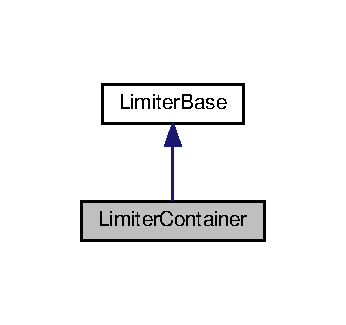
\includegraphics[width=166pt]{classLimiterContainer__inherit__graph}
\end{center}
\end{figure}


Collaboration diagram for Limiter\-Container\-:
\nopagebreak
\begin{figure}[H]
\begin{center}
\leavevmode
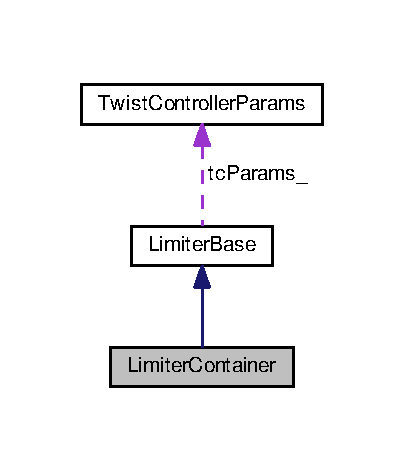
\includegraphics[width=194pt]{classLimiterContainer__coll__graph}
\end{center}
\end{figure}
\subsection*{Public Member Functions}
\begin{DoxyCompactItemize}
\item 
virtual K\-D\-L\-::\-Jnt\-Array \hyperlink{classLimiterContainer_a4df93d61aeb9e44c30127a1a2c8d0bd9}{enforce\-Limits} (const K\-D\-L\-::\-Jnt\-Array \&q\-\_\-dot\-\_\-ik, const K\-D\-L\-::\-Jnt\-Array \&q) const 
\item 
void \hyperlink{classLimiterContainer_a28eac48f36b165d02c86449189aacea2}{init} ()
\item 
virtual \hyperlink{classLimiterContainer_a4284c7a1f5094fbe24e0cd51f7bda6ab}{$\sim$\-Limiter\-Container} ()
\item 
\hypertarget{classLimiterContainer_a0aac7f3db0d1639b8bf38365e6e4a34c}{{\bfseries Limiter\-Container} (const \hyperlink{structTwistControllerParams}{Twist\-Controller\-Params} \&tc\-Params, const K\-D\-L\-::\-Chain \&chain)}\label{classLimiterContainer_a0aac7f3db0d1639b8bf38365e6e4a34c}

\end{DoxyCompactItemize}
\subsection*{Protected Types}
\begin{DoxyCompactItemize}
\item 
\hypertarget{classLimiterContainer_a32daab69a85e6f3ec090c9be462a88e0}{typedef std\-::vector$<$ const \\*
\hyperlink{classLimiterBase}{Limiter\-Base} $\ast$ $>$\\*
\-::const\-\_\-iterator {\bfseries lim\-Iter}}\label{classLimiterContainer_a32daab69a85e6f3ec090c9be462a88e0}

\end{DoxyCompactItemize}
\subsection*{Protected Member Functions}
\begin{DoxyCompactItemize}
\item 
void \hyperlink{classLimiterContainer_aef4914ff51be7ed8c563d47de9f316e8}{add} (const \hyperlink{classLimiterBase}{Limiter\-Base} $\ast$lb)
\item 
void \hyperlink{classLimiterContainer_a62b339d250d1d68fda7404d6fe89468b}{erase\-All} ()
\end{DoxyCompactItemize}
\subsection*{Protected Attributes}
\begin{DoxyCompactItemize}
\item 
\hypertarget{classLimiterContainer_a6fefcd7cc1cb4b8f029ce02013d2f5de}{std\-::vector$<$ const \hyperlink{classLimiterBase}{Limiter\-Base} $\ast$ $>$ {\bfseries limiters}}\label{classLimiterContainer_a6fefcd7cc1cb4b8f029ce02013d2f5de}

\end{DoxyCompactItemize}


\subsection{Detailed Description}
Container for limiters, implementing interface methods. 

\subsection{Constructor \& Destructor Documentation}
\hypertarget{classLimiterContainer_a4284c7a1f5094fbe24e0cd51f7bda6ab}{\index{Limiter\-Container@{Limiter\-Container}!$\sim$\-Limiter\-Container@{$\sim$\-Limiter\-Container}}
\index{$\sim$\-Limiter\-Container@{$\sim$\-Limiter\-Container}!LimiterContainer@{Limiter\-Container}}
\subsubsection[{$\sim$\-Limiter\-Container}]{\setlength{\rightskip}{0pt plus 5cm}Limiter\-Container\-::$\sim$\-Limiter\-Container (
\begin{DoxyParamCaption}
{}
\end{DoxyParamCaption}
)\hspace{0.3cm}{\ttfamily [virtual]}}}\label{classLimiterContainer_a4284c7a1f5094fbe24e0cd51f7bda6ab}
Destruction of the whole container 

Here is the call graph for this function\-:
\nopagebreak
\begin{figure}[H]
\begin{center}
\leavevmode
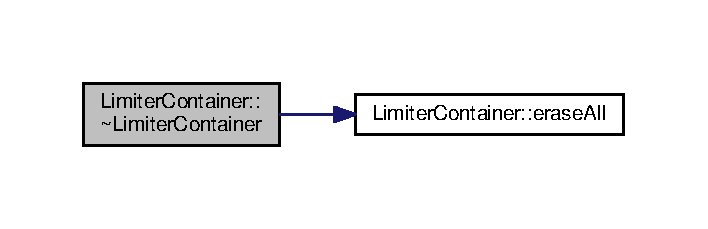
\includegraphics[width=340pt]{classLimiterContainer_a4284c7a1f5094fbe24e0cd51f7bda6ab_cgraph}
\end{center}
\end{figure}




\subsection{Member Function Documentation}
\hypertarget{classLimiterContainer_aef4914ff51be7ed8c563d47de9f316e8}{\index{Limiter\-Container@{Limiter\-Container}!add@{add}}
\index{add@{add}!LimiterContainer@{Limiter\-Container}}
\subsubsection[{add}]{\setlength{\rightskip}{0pt plus 5cm}void Limiter\-Container\-::add (
\begin{DoxyParamCaption}
\item[{const {\bf Limiter\-Base} $\ast$}]{lb}
\end{DoxyParamCaption}
)\hspace{0.3cm}{\ttfamily [protected]}}}\label{classLimiterContainer_aef4914ff51be7ed8c563d47de9f316e8}
Add method 
\begin{DoxyParams}{Parameters}
{\em lb} & An implementation of a limiter.\\
\hline
\end{DoxyParams}
Adding new limiters to the vector. 

Here is the caller graph for this function\-:
\nopagebreak
\begin{figure}[H]
\begin{center}
\leavevmode
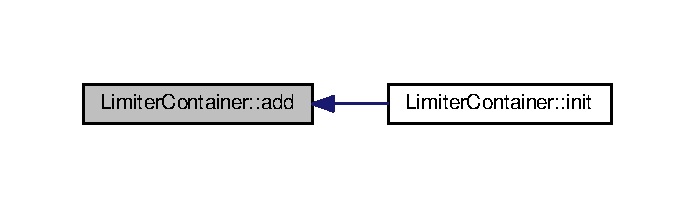
\includegraphics[width=334pt]{classLimiterContainer_aef4914ff51be7ed8c563d47de9f316e8_icgraph}
\end{center}
\end{figure}


\hypertarget{classLimiterContainer_a4df93d61aeb9e44c30127a1a2c8d0bd9}{\index{Limiter\-Container@{Limiter\-Container}!enforce\-Limits@{enforce\-Limits}}
\index{enforce\-Limits@{enforce\-Limits}!LimiterContainer@{Limiter\-Container}}
\subsubsection[{enforce\-Limits}]{\setlength{\rightskip}{0pt plus 5cm}K\-D\-L\-::\-Jnt\-Array Limiter\-Container\-::enforce\-Limits (
\begin{DoxyParamCaption}
\item[{const K\-D\-L\-::\-Jnt\-Array \&}]{q\-\_\-dot\-\_\-ik, }
\item[{const K\-D\-L\-::\-Jnt\-Array \&}]{q}
\end{DoxyParamCaption}
) const\hspace{0.3cm}{\ttfamily [virtual]}}}\label{classLimiterContainer_a4df93d61aeb9e44c30127a1a2c8d0bd9}
Specific implementation of enforce\-Limits-\/method. See base class \hyperlink{classLimiterBase}{Limiter\-Base} for more details on params and returns.

This implementation calls enforce limits on all registered Limiters in the limiters vector. The method is based on the last calculation of q\-\_\-dot. 

Implements \hyperlink{classLimiterBase_a1755edebc0cacfd79f945852ead8ae04}{Limiter\-Base}.

\hypertarget{classLimiterContainer_a62b339d250d1d68fda7404d6fe89468b}{\index{Limiter\-Container@{Limiter\-Container}!erase\-All@{erase\-All}}
\index{erase\-All@{erase\-All}!LimiterContainer@{Limiter\-Container}}
\subsubsection[{erase\-All}]{\setlength{\rightskip}{0pt plus 5cm}void Limiter\-Container\-::erase\-All (
\begin{DoxyParamCaption}
{}
\end{DoxyParamCaption}
)\hspace{0.3cm}{\ttfamily [protected]}}}\label{classLimiterContainer_a62b339d250d1d68fda7404d6fe89468b}
Erase all

Deletes all limiters and clears the vector holding them. 

Here is the caller graph for this function\-:
\nopagebreak
\begin{figure}[H]
\begin{center}
\leavevmode
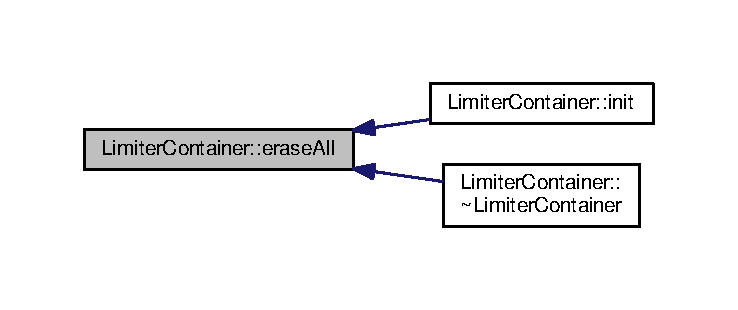
\includegraphics[width=350pt]{classLimiterContainer_a62b339d250d1d68fda7404d6fe89468b_icgraph}
\end{center}
\end{figure}


\hypertarget{classLimiterContainer_a28eac48f36b165d02c86449189aacea2}{\index{Limiter\-Container@{Limiter\-Container}!init@{init}}
\index{init@{init}!LimiterContainer@{Limiter\-Container}}
\subsubsection[{init}]{\setlength{\rightskip}{0pt plus 5cm}void Limiter\-Container\-::init (
\begin{DoxyParamCaption}
{}
\end{DoxyParamCaption}
)}}\label{classLimiterContainer_a28eac48f36b165d02c86449189aacea2}
Initialization for the container.

Building the limiters vector according the the chosen parameters. 

Here is the call graph for this function\-:
\nopagebreak
\begin{figure}[H]
\begin{center}
\leavevmode
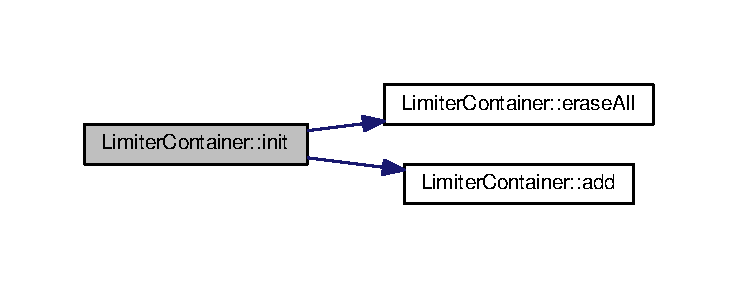
\includegraphics[width=350pt]{classLimiterContainer_a28eac48f36b165d02c86449189aacea2_cgraph}
\end{center}
\end{figure}




The documentation for this class was generated from the following files\-:\begin{DoxyCompactItemize}
\item 
/home/fxm-\/cm/catkin\-\_\-ws/src/cob\-\_\-control/cob\-\_\-twist\-\_\-controller/include/cob\-\_\-twist\-\_\-controller/limiters/\hyperlink{limiter_8h}{limiter.\-h}\item 
/home/fxm-\/cm/catkin\-\_\-ws/src/cob\-\_\-control/cob\-\_\-twist\-\_\-controller/src/limiters/\hyperlink{limiter_8cpp}{limiter.\-cpp}\end{DoxyCompactItemize}

\hypertarget{classLimiterIndividualJointPositions}{\section{Limiter\-Individual\-Joint\-Positions Class Reference}
\label{classLimiterIndividualJointPositions}\index{Limiter\-Individual\-Joint\-Positions@{Limiter\-Individual\-Joint\-Positions}}
}


Class for a limiter, declaring a method to limit joint positions individually.  




{\ttfamily \#include $<$limiter.\-h$>$}



Inheritance diagram for Limiter\-Individual\-Joint\-Positions\-:
\nopagebreak
\begin{figure}[H]
\begin{center}
\leavevmode
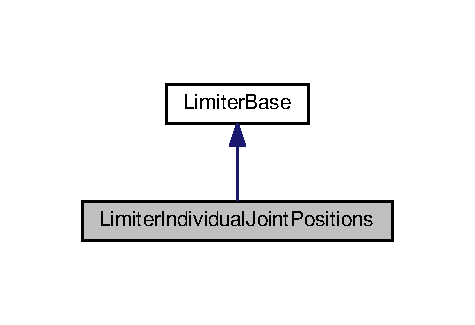
\includegraphics[width=228pt]{classLimiterIndividualJointPositions__inherit__graph}
\end{center}
\end{figure}


Collaboration diagram for Limiter\-Individual\-Joint\-Positions\-:
\nopagebreak
\begin{figure}[H]
\begin{center}
\leavevmode
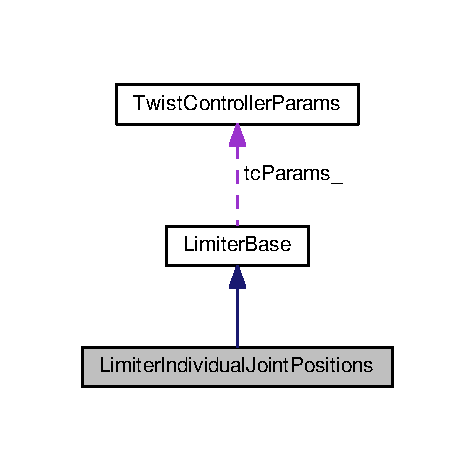
\includegraphics[width=228pt]{classLimiterIndividualJointPositions__coll__graph}
\end{center}
\end{figure}
\subsection*{Public Member Functions}
\begin{DoxyCompactItemize}
\item 
virtual K\-D\-L\-::\-Jnt\-Array \hyperlink{classLimiterIndividualJointPositions_aa5a977c62d490397ae7e685a4d7f1f94}{enforce\-Limits} (const K\-D\-L\-::\-Jnt\-Array \&q\-\_\-dot\-\_\-ik, const K\-D\-L\-::\-Jnt\-Array \&q) const 
\item 
\hypertarget{classLimiterIndividualJointPositions_ab90884cd95d724af590af7415b6b045d}{{\bfseries Limiter\-Individual\-Joint\-Positions} (const \hyperlink{structTwistControllerParams}{Twist\-Controller\-Params} \&tc\-Params, const K\-D\-L\-::\-Chain \&chain)}\label{classLimiterIndividualJointPositions_ab90884cd95d724af590af7415b6b045d}

\end{DoxyCompactItemize}
\subsection*{Additional Inherited Members}


\subsection{Detailed Description}
Class for a limiter, declaring a method to limit joint positions individually. 

\subsection{Member Function Documentation}
\hypertarget{classLimiterIndividualJointPositions_aa5a977c62d490397ae7e685a4d7f1f94}{\index{Limiter\-Individual\-Joint\-Positions@{Limiter\-Individual\-Joint\-Positions}!enforce\-Limits@{enforce\-Limits}}
\index{enforce\-Limits@{enforce\-Limits}!LimiterIndividualJointPositions@{Limiter\-Individual\-Joint\-Positions}}
\subsubsection[{enforce\-Limits}]{\setlength{\rightskip}{0pt plus 5cm}K\-D\-L\-::\-Jnt\-Array Limiter\-Individual\-Joint\-Positions\-::enforce\-Limits (
\begin{DoxyParamCaption}
\item[{const K\-D\-L\-::\-Jnt\-Array \&}]{q\-\_\-dot\-\_\-ik, }
\item[{const K\-D\-L\-::\-Jnt\-Array \&}]{q}
\end{DoxyParamCaption}
) const\hspace{0.3cm}{\ttfamily [virtual]}}}\label{classLimiterIndividualJointPositions_aa5a977c62d490397ae7e685a4d7f1f94}
Specific implementation of enforce\-Limits-\/method. See base class \hyperlink{classLimiterBase}{Limiter\-Base} for more details on params and returns.

This implementation calculates limits for the joint positions without keeping the direction. Then for each corresponding joint velocity an individual factor for scaling is calculated and then used. 

Implements \hyperlink{classLimiterBase_a1755edebc0cacfd79f945852ead8ae04}{Limiter\-Base}.



The documentation for this class was generated from the following files\-:\begin{DoxyCompactItemize}
\item 
/home/fxm-\/cm/catkin\-\_\-ws/src/cob\-\_\-control/cob\-\_\-twist\-\_\-controller/include/cob\-\_\-twist\-\_\-controller/limiters/\hyperlink{limiter_8h}{limiter.\-h}\item 
/home/fxm-\/cm/catkin\-\_\-ws/src/cob\-\_\-control/cob\-\_\-twist\-\_\-controller/src/limiters/\hyperlink{limiter_8cpp}{limiter.\-cpp}\end{DoxyCompactItemize}

\hypertarget{classLimiterIndividualJointVelocities}{\section{Limiter\-Individual\-Joint\-Velocities Class Reference}
\label{classLimiterIndividualJointVelocities}\index{Limiter\-Individual\-Joint\-Velocities@{Limiter\-Individual\-Joint\-Velocities}}
}


Class for joint velocity limiter (individually scaled -\/$>$ changes direction), implementing interface methods.  




{\ttfamily \#include $<$limiter.\-h$>$}



Inheritance diagram for Limiter\-Individual\-Joint\-Velocities\-:
\nopagebreak
\begin{figure}[H]
\begin{center}
\leavevmode
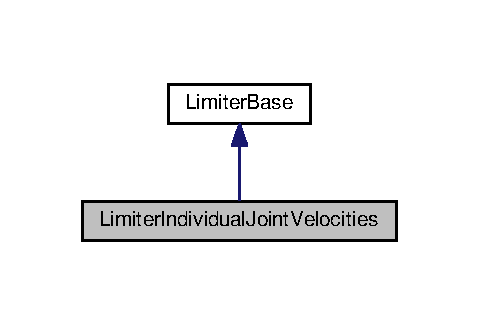
\includegraphics[width=230pt]{classLimiterIndividualJointVelocities__inherit__graph}
\end{center}
\end{figure}


Collaboration diagram for Limiter\-Individual\-Joint\-Velocities\-:
\nopagebreak
\begin{figure}[H]
\begin{center}
\leavevmode
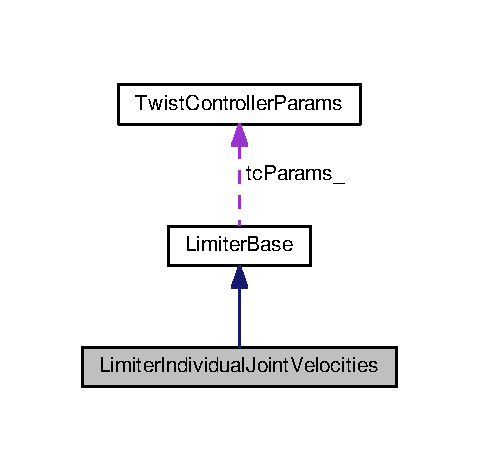
\includegraphics[width=230pt]{classLimiterIndividualJointVelocities__coll__graph}
\end{center}
\end{figure}
\subsection*{Public Member Functions}
\begin{DoxyCompactItemize}
\item 
virtual K\-D\-L\-::\-Jnt\-Array \hyperlink{classLimiterIndividualJointVelocities_a298fddd7c5f1c806eb7efeb9a18a0cf8}{enforce\-Limits} (const K\-D\-L\-::\-Jnt\-Array \&q\-\_\-dot\-\_\-ik, const K\-D\-L\-::\-Jnt\-Array \&q) const 
\item 
\hypertarget{classLimiterIndividualJointVelocities_a0d5c210fe2d43a1f2e692323763f0f3b}{{\bfseries Limiter\-Individual\-Joint\-Velocities} (const \hyperlink{structTwistControllerParams}{Twist\-Controller\-Params} \&tc\-Params, const K\-D\-L\-::\-Chain \&chain)}\label{classLimiterIndividualJointVelocities_a0d5c210fe2d43a1f2e692323763f0f3b}

\end{DoxyCompactItemize}
\subsection*{Additional Inherited Members}


\subsection{Detailed Description}
Class for joint velocity limiter (individually scaled -\/$>$ changes direction), implementing interface methods. 

\subsection{Member Function Documentation}
\hypertarget{classLimiterIndividualJointVelocities_a298fddd7c5f1c806eb7efeb9a18a0cf8}{\index{Limiter\-Individual\-Joint\-Velocities@{Limiter\-Individual\-Joint\-Velocities}!enforce\-Limits@{enforce\-Limits}}
\index{enforce\-Limits@{enforce\-Limits}!LimiterIndividualJointVelocities@{Limiter\-Individual\-Joint\-Velocities}}
\subsubsection[{enforce\-Limits}]{\setlength{\rightskip}{0pt plus 5cm}K\-D\-L\-::\-Jnt\-Array Limiter\-Individual\-Joint\-Velocities\-::enforce\-Limits (
\begin{DoxyParamCaption}
\item[{const K\-D\-L\-::\-Jnt\-Array \&}]{q\-\_\-dot\-\_\-ik, }
\item[{const K\-D\-L\-::\-Jnt\-Array \&}]{q}
\end{DoxyParamCaption}
) const\hspace{0.3cm}{\ttfamily [virtual]}}}\label{classLimiterIndividualJointVelocities_a298fddd7c5f1c806eb7efeb9a18a0cf8}
Specific implementation of enforce\-Limits-\/method. See base class \hyperlink{classLimiterBase}{Limiter\-Base} for more details on params and returns.

This implementation calculates limits for the joint velocities without keeping the direction. For each joint velocity in the vector an individual factor for scaling is calculated and used. 

Implements \hyperlink{classLimiterBase_a1755edebc0cacfd79f945852ead8ae04}{Limiter\-Base}.



The documentation for this class was generated from the following files\-:\begin{DoxyCompactItemize}
\item 
/home/fxm-\/cm/catkin\-\_\-ws/src/cob\-\_\-control/cob\-\_\-twist\-\_\-controller/include/cob\-\_\-twist\-\_\-controller/limiters/\hyperlink{limiter_8h}{limiter.\-h}\item 
/home/fxm-\/cm/catkin\-\_\-ws/src/cob\-\_\-control/cob\-\_\-twist\-\_\-controller/src/limiters/\hyperlink{limiter_8cpp}{limiter.\-cpp}\end{DoxyCompactItemize}

\hypertarget{classSolverFactory}{\section{Solver\-Factory$<$ T $>$ Class Template Reference}
\label{classSolverFactory}\index{Solver\-Factory$<$ T $>$@{Solver\-Factory$<$ T $>$}}
}


Abstract base class defining interfaces for the creation of a specific solver.  




{\ttfamily \#include $<$solver\-\_\-factory.\-h$>$}



Inheritance diagram for Solver\-Factory$<$ T $>$\-:
\nopagebreak
\begin{figure}[H]
\begin{center}
\leavevmode
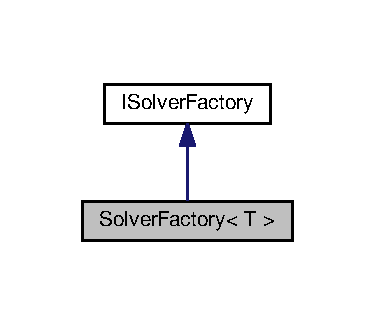
\includegraphics[width=180pt]{classSolverFactory__inherit__graph}
\end{center}
\end{figure}


Collaboration diagram for Solver\-Factory$<$ T $>$\-:
\nopagebreak
\begin{figure}[H]
\begin{center}
\leavevmode
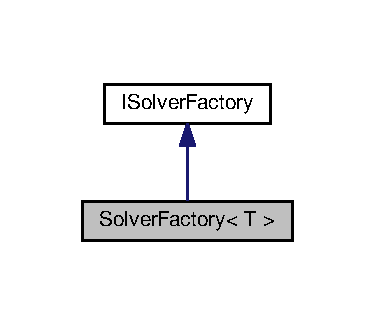
\includegraphics[width=180pt]{classSolverFactory__coll__graph}
\end{center}
\end{figure}
\subsection*{Public Member Functions}
\begin{DoxyCompactItemize}
\item 
Eigen\-::\-Matrix\-Xd \hyperlink{classSolverFactory_a1dfa247805c6c9ec5a0adf36a710366d}{calculate\-Joint\-Velocities} (\hyperlink{structAugmentedSolverParams}{Augmented\-Solver\-Params} \&as\-Params, Matrix6\-Xd \&jacobian\-Data, const Eigen\-::\-Vector\-Xd \&in\-Cart\-Velocities, const K\-D\-L\-::\-Jnt\-Array \&q, const K\-D\-L\-::\-Jnt\-Array \&last\-\_\-q\-\_\-dot, double damping\-Factor) const 
\end{DoxyCompactItemize}
\subsection*{Protected Member Functions}
\begin{DoxyCompactItemize}
\item 
T $\ast$ \hyperlink{classSolverFactory_a49a73417f779159054fee4f6218ce7c8}{create\-Solver} (\hyperlink{structAugmentedSolverParams}{Augmented\-Solver\-Params} \&as\-Params, Matrix6\-Xd \&jacobian\-Data) const 
\end{DoxyCompactItemize}


\subsection{Detailed Description}
\subsubsection*{template$<$typename T$>$class Solver\-Factory$<$ T $>$}

Abstract base class defining interfaces for the creation of a specific solver. 

\subsection{Member Function Documentation}
\hypertarget{classSolverFactory_a1dfa247805c6c9ec5a0adf36a710366d}{\index{Solver\-Factory@{Solver\-Factory}!calculate\-Joint\-Velocities@{calculate\-Joint\-Velocities}}
\index{calculate\-Joint\-Velocities@{calculate\-Joint\-Velocities}!SolverFactory@{Solver\-Factory}}
\subsubsection[{calculate\-Joint\-Velocities}]{\setlength{\rightskip}{0pt plus 5cm}template$<$typename T $>$ Eigen\-::\-Matrix\-Xd {\bf Solver\-Factory}$<$ T $>$\-::calculate\-Joint\-Velocities (
\begin{DoxyParamCaption}
\item[{{\bf Augmented\-Solver\-Params} \&}]{as\-Params, }
\item[{Matrix6\-Xd \&}]{jacobian\-Data, }
\item[{const Eigen\-::\-Vector\-Xd \&}]{in\-Cart\-Velocities, }
\item[{const K\-D\-L\-::\-Jnt\-Array \&}]{q, }
\item[{const K\-D\-L\-::\-Jnt\-Array \&}]{last\-\_\-q\-\_\-dot, }
\item[{double}]{damping\-Factor}
\end{DoxyParamCaption}
) const\hspace{0.3cm}{\ttfamily [inline]}, {\ttfamily [virtual]}}}\label{classSolverFactory_a1dfa247805c6c9ec5a0adf36a710366d}
The base calculation method to calculate joint velocities out of input velocities (cartesian space). Creates a solver according to implemented create\-Solver-\/method (in subclass). Use the specialized solve-\/method to calculate new joint velocities. 
\begin{DoxyParams}{Parameters}
{\em as\-Params} & References the augmented solver parameters. \\
\hline
{\em jacobian\-Data} & References the current Jacobian (matrix data only). \\
\hline
{\em jacobian\-Data\-Transposed} & References the current Jacobian transpose (matrix data only). \\
\hline
{\em in\-Cart\-Velocities} & The input velocities vector (in cartesian space). \\
\hline
{\em q} & The current joint positions. \\
\hline
{\em last\-\_\-q\-\_\-dot} & The last joint velocities. \\
\hline
{\em damping\-Factor} & The damping factor corresponding to damping method. \\
\hline
\end{DoxyParams}
\begin{DoxyReturn}{Returns}
Joint velocities in a (m x 1)-\/\-Matrix. 
\end{DoxyReturn}


Implements \hyperlink{classISolverFactory}{I\-Solver\-Factory}.



Here is the call graph for this function\-:
\nopagebreak
\begin{figure}[H]
\begin{center}
\leavevmode
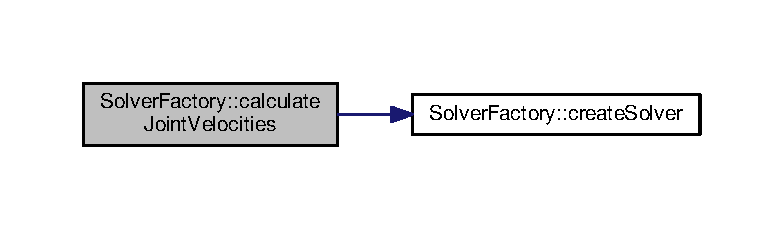
\includegraphics[width=350pt]{classSolverFactory_a1dfa247805c6c9ec5a0adf36a710366d_cgraph}
\end{center}
\end{figure}


\hypertarget{classSolverFactory_a49a73417f779159054fee4f6218ce7c8}{\index{Solver\-Factory@{Solver\-Factory}!create\-Solver@{create\-Solver}}
\index{create\-Solver@{create\-Solver}!SolverFactory@{Solver\-Factory}}
\subsubsection[{create\-Solver}]{\setlength{\rightskip}{0pt plus 5cm}template$<$typename T $>$ T$\ast$ {\bf Solver\-Factory}$<$ T $>$\-::create\-Solver (
\begin{DoxyParamCaption}
\item[{{\bf Augmented\-Solver\-Params} \&}]{as\-Params, }
\item[{Matrix6\-Xd \&}]{jacobian\-Data}
\end{DoxyParamCaption}
) const\hspace{0.3cm}{\ttfamily [inline]}, {\ttfamily [protected]}}}\label{classSolverFactory_a49a73417f779159054fee4f6218ce7c8}
The interface method to create a specific solver to solve the inverse kinematics problem. 
\begin{DoxyParams}{Parameters}
{\em as\-Params} & References the augmented solver parameters. \\
\hline
{\em jacobian\-Data} & References the current Jacobian (matrix data only). \\
\hline
{\em jacobian\-Data\-Transposed} & References the current Jacobian transpose (matrix data only). \\
\hline
\end{DoxyParams}
\begin{DoxyReturn}{Returns}
A specific solver. 
\end{DoxyReturn}


Here is the caller graph for this function\-:
\nopagebreak
\begin{figure}[H]
\begin{center}
\leavevmode
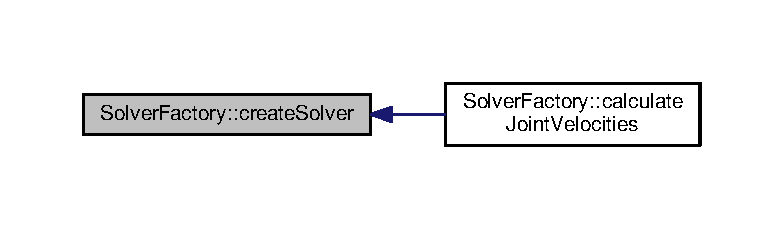
\includegraphics[width=350pt]{classSolverFactory_a49a73417f779159054fee4f6218ce7c8_icgraph}
\end{center}
\end{figure}




The documentation for this class was generated from the following file\-:\begin{DoxyCompactItemize}
\item 
/home/fxm-\/cm/catkin\-\_\-ws/src/cob\-\_\-control/cob\-\_\-twist\-\_\-controller/include/cob\-\_\-twist\-\_\-controller/constraint\-\_\-solvers/factories/\hyperlink{solver__factory_8h}{solver\-\_\-factory.\-h}\end{DoxyCompactItemize}

\hypertarget{structTwistControllerParams}{\section{Twist\-Controller\-Params Struct Reference}
\label{structTwistControllerParams}\index{Twist\-Controller\-Params@{Twist\-Controller\-Params}}
}
\subsection*{Public Attributes}
\begin{DoxyCompactItemize}
\item 
\hypertarget{structTwistControllerParams_a69524f6ddafd01ee5b5622aaedf4a255}{uint8\-\_\-t {\bfseries dof}}\label{structTwistControllerParams_a69524f6ddafd01ee5b5622aaedf4a255}

\item 
\hypertarget{structTwistControllerParams_a76a09cf3f2fcaa612a318ddb68d06a89}{bool {\bfseries base\-\_\-active}}\label{structTwistControllerParams_a76a09cf3f2fcaa612a318ddb68d06a89}

\item 
\hypertarget{structTwistControllerParams_ab1f7484bf017d7c6c0be8ca97b6a90fc}{bool {\bfseries base\-\_\-compensation}}\label{structTwistControllerParams_ab1f7484bf017d7c6c0be8ca97b6a90fc}

\item 
\hypertarget{structTwistControllerParams_a01732686f0558b9ff1bb233d4272b3f1}{double {\bfseries max\-\_\-vel\-\_\-lin}}\label{structTwistControllerParams_a01732686f0558b9ff1bb233d4272b3f1}

\item 
\hypertarget{structTwistControllerParams_af4a0c5a8a8b9061952de82b1cc2745f8}{double {\bfseries max\-\_\-vel\-\_\-rot}}\label{structTwistControllerParams_af4a0c5a8a8b9061952de82b1cc2745f8}

\item 
\hypertarget{structTwistControllerParams_ac7f0079a39420df534f75cbdfb111659}{double {\bfseries max\-\_\-vel\-\_\-lin\-\_\-base}}\label{structTwistControllerParams_ac7f0079a39420df534f75cbdfb111659}

\item 
\hypertarget{structTwistControllerParams_a258564a070a6d212ce627ffc735e3e3b}{double {\bfseries max\-\_\-vel\-\_\-rot\-\_\-base}}\label{structTwistControllerParams_a258564a070a6d212ce627ffc735e3e3b}

\item 
\hypertarget{structTwistControllerParams_a625ee1a3f8f44b72bd08a940ba079560}{double {\bfseries tolerance}}\label{structTwistControllerParams_a625ee1a3f8f44b72bd08a940ba079560}

\item 
\hypertarget{structTwistControllerParams_a18da932a0624fb5499507392175132cc}{bool {\bfseries keep\-\_\-direction}}\label{structTwistControllerParams_a18da932a0624fb5499507392175132cc}

\item 
\hypertarget{structTwistControllerParams_af84880928b522f0be3d1ed4558dab106}{bool {\bfseries enforce\-\_\-pos\-\_\-limits}}\label{structTwistControllerParams_af84880928b522f0be3d1ed4558dab106}

\item 
\hypertarget{structTwistControllerParams_a1b2aff868e1d52ec02aace9d36131a20}{bool {\bfseries enforce\-\_\-vel\-\_\-limits}}\label{structTwistControllerParams_a1b2aff868e1d52ec02aace9d36131a20}

\item 
\hypertarget{structTwistControllerParams_a86b1bc3844ddff53b417a19ccfc460be}{std\-::vector$<$ double $>$ {\bfseries limits\-\_\-vel}}\label{structTwistControllerParams_a86b1bc3844ddff53b417a19ccfc460be}

\item 
\hypertarget{structTwistControllerParams_af7544aceba6c8ab3397d2ee8dcbc5b4e}{std\-::vector$<$ double $>$ {\bfseries limits\-\_\-min}}\label{structTwistControllerParams_af7544aceba6c8ab3397d2ee8dcbc5b4e}

\item 
\hypertarget{structTwistControllerParams_a133e7f291118bdbda18a67df38eac6a8}{std\-::vector$<$ double $>$ {\bfseries limits\-\_\-max}}\label{structTwistControllerParams_a133e7f291118bdbda18a67df38eac6a8}

\end{DoxyCompactItemize}


The documentation for this struct was generated from the following file\-:\begin{DoxyCompactItemize}
\item 
/home/fxm-\/cm/catkin\-\_\-ws/src/cob\-\_\-control/cob\-\_\-twist\-\_\-controller/include/cob\-\_\-twist\-\_\-controller/\hyperlink{cob__twist__controller__data__types_8h}{cob\-\_\-twist\-\_\-controller\-\_\-data\-\_\-types.\-h}\end{DoxyCompactItemize}

\hypertarget{classUnconstraintSolver}{\section{Unconstraint\-Solver Class Reference}
\label{classUnconstraintSolver}\index{Unconstraint\-Solver@{Unconstraint\-Solver}}
}


Inheritance diagram for Unconstraint\-Solver\-:
\nopagebreak
\begin{figure}[H]
\begin{center}
\leavevmode
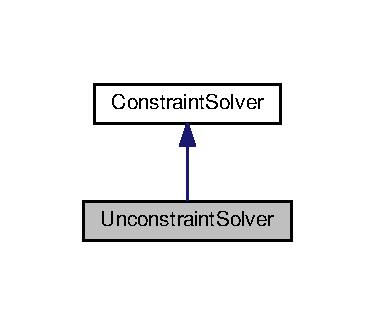
\includegraphics[width=180pt]{classUnconstraintSolver__inherit__graph}
\end{center}
\end{figure}


Collaboration diagram for Unconstraint\-Solver\-:
\nopagebreak
\begin{figure}[H]
\begin{center}
\leavevmode
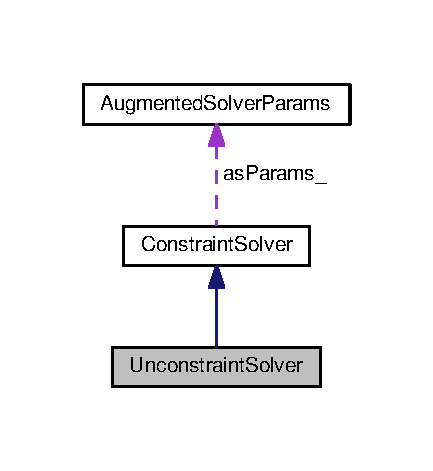
\includegraphics[width=208pt]{classUnconstraintSolver__coll__graph}
\end{center}
\end{figure}
\subsection*{Public Member Functions}
\begin{DoxyCompactItemize}
\item 
virtual Eigen\-::\-Matrix\-Xd \hyperlink{classUnconstraintSolver_a72e63efba891d2a55f4c95746b8d7b33}{solve} (const Eigen\-::\-Vector\-Xd \&in\-Cart\-Velocities, const K\-D\-L\-::\-Jnt\-Array \&q, const K\-D\-L\-::\-Jnt\-Array \&last\-\_\-q\-\_\-dot) const 
\item 
\hypertarget{classUnconstraintSolver_a3018879def8a39783ba4de35e27198d9}{{\bfseries Unconstraint\-Solver} (\hyperlink{structAugmentedSolverParams}{Augmented\-Solver\-Params} \&as\-Params, Matrix6\-Xd \&jacobian\-Data)}\label{classUnconstraintSolver_a3018879def8a39783ba4de35e27198d9}

\end{DoxyCompactItemize}
\subsection*{Additional Inherited Members}


\subsection{Member Function Documentation}
\hypertarget{classUnconstraintSolver_a72e63efba891d2a55f4c95746b8d7b33}{\index{Unconstraint\-Solver@{Unconstraint\-Solver}!solve@{solve}}
\index{solve@{solve}!UnconstraintSolver@{Unconstraint\-Solver}}
\subsubsection[{solve}]{\setlength{\rightskip}{0pt plus 5cm}Eigen\-::\-Matrix\-Xd Unconstraint\-Solver\-::solve (
\begin{DoxyParamCaption}
\item[{const Eigen\-::\-Vector\-Xd \&}]{in\-Cart\-Velocities, }
\item[{const K\-D\-L\-::\-Jnt\-Array \&}]{q, }
\item[{const K\-D\-L\-::\-Jnt\-Array \&}]{last\-\_\-q\-\_\-dot}
\end{DoxyParamCaption}
) const\hspace{0.3cm}{\ttfamily [virtual]}}}\label{classUnconstraintSolver_a72e63efba891d2a55f4c95746b8d7b33}
Specific implementation of solve-\/method to solve I\-K problem without any constraints. See base class \hyperlink{classConstraintSolver}{Constraint\-Solver} for more details on params and returns.

Implementation of a default solve-\/method for the inverse kinematics problem. It calculates the pseudo-\/inverse of the Jacobian via the base implementation of calculate\-Pinv\-Jacobian\-By\-S\-V\-D. With the pseudo-\/inverse the joint velocity vector is calculated. 

Implements \hyperlink{classConstraintSolver_a6208240cb2dc47fdd9adfc3a069408cd}{Constraint\-Solver}.



Here is the call graph for this function\-:
\nopagebreak
\begin{figure}[H]
\begin{center}
\leavevmode
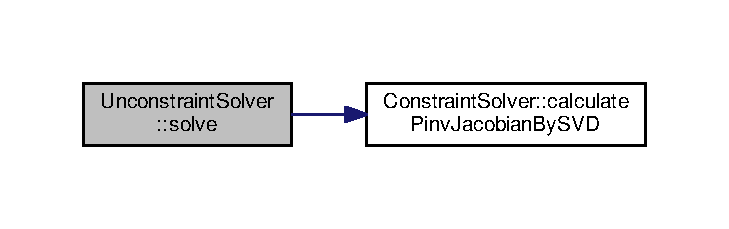
\includegraphics[width=350pt]{classUnconstraintSolver_a72e63efba891d2a55f4c95746b8d7b33_cgraph}
\end{center}
\end{figure}




The documentation for this class was generated from the following files\-:\begin{DoxyCompactItemize}
\item 
/home/fxm-\/cm/catkin\-\_\-ws/src/cob\-\_\-control/cob\-\_\-twist\-\_\-controller/include/cob\-\_\-twist\-\_\-controller/constraint\-\_\-solvers/solvers/\hyperlink{unconstraint__solver_8h}{unconstraint\-\_\-solver.\-h}\item 
/home/fxm-\/cm/catkin\-\_\-ws/src/cob\-\_\-control/cob\-\_\-twist\-\_\-controller/src/constraint\-\_\-solvers/solvers/\hyperlink{unconstraint__solver_8cpp}{unconstraint\-\_\-solver.\-cpp}\end{DoxyCompactItemize}

\hypertarget{classWeightedLeastNormSolver}{\section{Weighted\-Least\-Norm\-Solver Class Reference}
\label{classWeightedLeastNormSolver}\index{Weighted\-Least\-Norm\-Solver@{Weighted\-Least\-Norm\-Solver}}
}


Implementation of \hyperlink{classConstraintSolver}{Constraint\-Solver} to solve inverse kinematics by using a weighted least norm.  




{\ttfamily \#include $<$weighted\-\_\-least\-\_\-norm\-\_\-solver.\-h$>$}



Inheritance diagram for Weighted\-Least\-Norm\-Solver\-:
\nopagebreak
\begin{figure}[H]
\begin{center}
\leavevmode
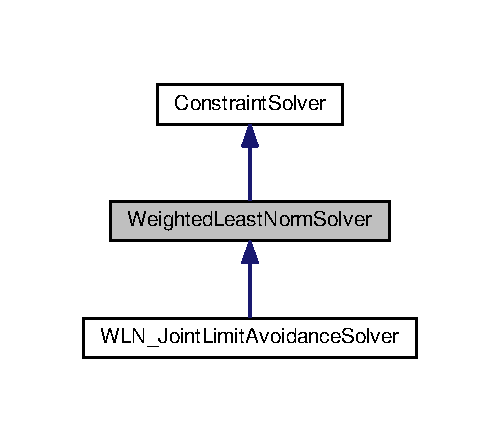
\includegraphics[width=240pt]{classWeightedLeastNormSolver__inherit__graph}
\end{center}
\end{figure}


Collaboration diagram for Weighted\-Least\-Norm\-Solver\-:
\nopagebreak
\begin{figure}[H]
\begin{center}
\leavevmode
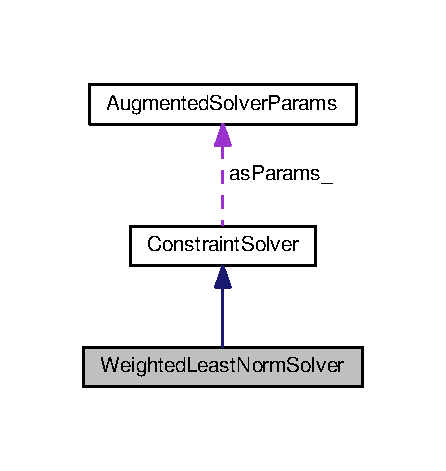
\includegraphics[width=214pt]{classWeightedLeastNormSolver__coll__graph}
\end{center}
\end{figure}
\subsection*{Public Member Functions}
\begin{DoxyCompactItemize}
\item 
virtual Eigen\-::\-Matrix\-Xd \hyperlink{classWeightedLeastNormSolver_a0868fb81e9e75999037d96b4a6407ce7}{solve} (const Eigen\-::\-Vector\-Xd \&in\-Cart\-Velocities, const K\-D\-L\-::\-Jnt\-Array \&q, const K\-D\-L\-::\-Jnt\-Array \&last\-\_\-q\-\_\-dot) const 
\item 
\hypertarget{classWeightedLeastNormSolver_aa5eeee99709044b47bc32a4cc1ca72dd}{{\bfseries Weighted\-Least\-Norm\-Solver} (\hyperlink{structAugmentedSolverParams}{Augmented\-Solver\-Params} \&as\-Params, Matrix6\-Xd \&jacobian\-Data)}\label{classWeightedLeastNormSolver_aa5eeee99709044b47bc32a4cc1ca72dd}

\end{DoxyCompactItemize}
\subsection*{Additional Inherited Members}


\subsection{Detailed Description}
Implementation of \hyperlink{classConstraintSolver}{Constraint\-Solver} to solve inverse kinematics by using a weighted least norm. 

\subsection{Member Function Documentation}
\hypertarget{classWeightedLeastNormSolver_a0868fb81e9e75999037d96b4a6407ce7}{\index{Weighted\-Least\-Norm\-Solver@{Weighted\-Least\-Norm\-Solver}!solve@{solve}}
\index{solve@{solve}!WeightedLeastNormSolver@{Weighted\-Least\-Norm\-Solver}}
\subsubsection[{solve}]{\setlength{\rightskip}{0pt plus 5cm}Eigen\-::\-Matrix\-Xd Weighted\-Least\-Norm\-Solver\-::solve (
\begin{DoxyParamCaption}
\item[{const Eigen\-::\-Vector\-Xd \&}]{in\-Cart\-Velocities, }
\item[{const K\-D\-L\-::\-Jnt\-Array \&}]{q, }
\item[{const K\-D\-L\-::\-Jnt\-Array \&}]{last\-\_\-q\-\_\-dot}
\end{DoxyParamCaption}
) const\hspace{0.3cm}{\ttfamily [virtual]}}}\label{classWeightedLeastNormSolver_a0868fb81e9e75999037d96b4a6407ce7}
Specific implementation of solve-\/method to solve I\-K problem with joint limit avoidance. See base class \hyperlink{classConstraintSolver}{Constraint\-Solver} for more details on params and returns.

Specific implementation of the solve method using a weighted least norm. This is done by calculation of a weighting which is dependent on inherited classes for the Jacobian. Uses the base implementation of calculate\-Pinv\-Jacobian\-By\-S\-V\-D to calculate the pseudo-\/inverse (weighted) Jacobian. 

Implements \hyperlink{classConstraintSolver_a6208240cb2dc47fdd9adfc3a069408cd}{Constraint\-Solver}.



Here is the call graph for this function\-:
\nopagebreak
\begin{figure}[H]
\begin{center}
\leavevmode
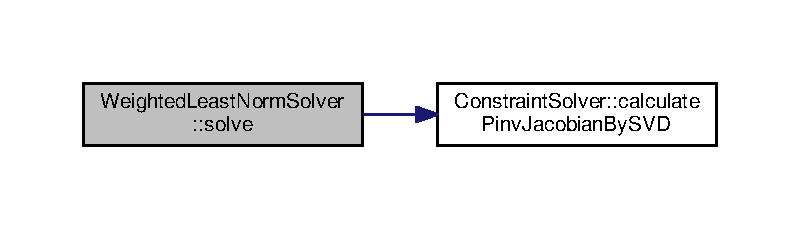
\includegraphics[width=350pt]{classWeightedLeastNormSolver_a0868fb81e9e75999037d96b4a6407ce7_cgraph}
\end{center}
\end{figure}




The documentation for this class was generated from the following files\-:\begin{DoxyCompactItemize}
\item 
/home/fxm-\/cm/catkin\-\_\-ws/src/cob\-\_\-control/cob\-\_\-twist\-\_\-controller/include/cob\-\_\-twist\-\_\-controller/constraint\-\_\-solvers/solvers/\hyperlink{weighted__least__norm__solver_8h}{weighted\-\_\-least\-\_\-norm\-\_\-solver.\-h}\item 
/home/fxm-\/cm/catkin\-\_\-ws/src/cob\-\_\-control/cob\-\_\-twist\-\_\-controller/src/constraint\-\_\-solvers/solvers/\hyperlink{weighted__least__norm__solver_8cpp}{weighted\-\_\-least\-\_\-norm\-\_\-solver.\-cpp}\end{DoxyCompactItemize}

\hypertarget{classWLN__JointLimitAvoidanceSolver}{\section{W\-L\-N\-\_\-\-Joint\-Limit\-Avoidance\-Solver Class Reference}
\label{classWLN__JointLimitAvoidanceSolver}\index{W\-L\-N\-\_\-\-Joint\-Limit\-Avoidance\-Solver@{W\-L\-N\-\_\-\-Joint\-Limit\-Avoidance\-Solver}}
}


{\ttfamily \#include $<$wln\-\_\-joint\-\_\-limit\-\_\-avoidance\-\_\-solver.\-h$>$}



Inheritance diagram for W\-L\-N\-\_\-\-Joint\-Limit\-Avoidance\-Solver\-:
\nopagebreak
\begin{figure}[H]
\begin{center}
\leavevmode
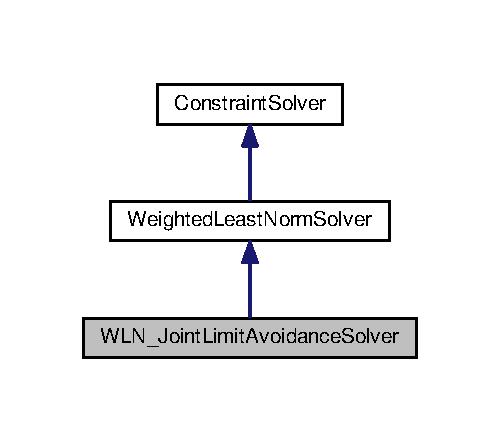
\includegraphics[width=240pt]{classWLN__JointLimitAvoidanceSolver__inherit__graph}
\end{center}
\end{figure}


Collaboration diagram for W\-L\-N\-\_\-\-Joint\-Limit\-Avoidance\-Solver\-:
\nopagebreak
\begin{figure}[H]
\begin{center}
\leavevmode
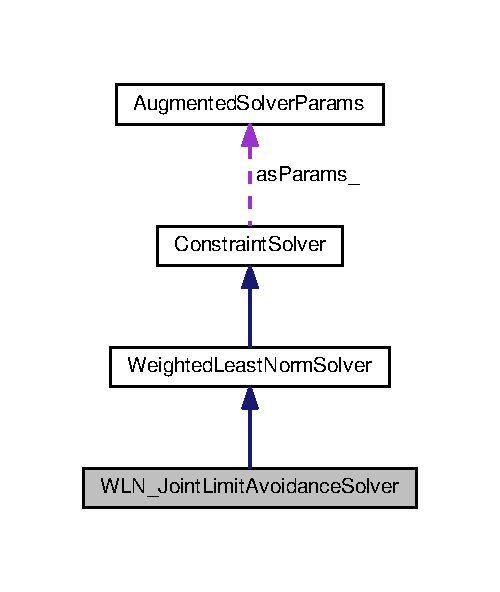
\includegraphics[width=240pt]{classWLN__JointLimitAvoidanceSolver__coll__graph}
\end{center}
\end{figure}
\subsection*{Public Member Functions}
\begin{DoxyCompactItemize}
\item 
\hypertarget{classWLN__JointLimitAvoidanceSolver_a943e85fe29f9ef0e1d1c30dc69add744}{{\bfseries W\-L\-N\-\_\-\-Joint\-Limit\-Avoidance\-Solver} (\hyperlink{structAugmentedSolverParams}{Augmented\-Solver\-Params} \&as\-Params, Matrix6\-Xd \&jacobian\-Data)}\label{classWLN__JointLimitAvoidanceSolver_a943e85fe29f9ef0e1d1c30dc69add744}

\end{DoxyCompactItemize}
\subsection*{Additional Inherited Members}


\subsection{Detailed Description}
Implementation of \hyperlink{classConstraintSolver}{Constraint\-Solver} to solve inverse kinematics with joint limit avoidance Uses solve method of the \hyperlink{classWeightedLeastNormSolver}{Weighted\-Least\-Norm\-Solver} 

The documentation for this class was generated from the following files\-:\begin{DoxyCompactItemize}
\item 
/home/fxm-\/cm/catkin\-\_\-ws/src/cob\-\_\-control/cob\-\_\-twist\-\_\-controller/include/cob\-\_\-twist\-\_\-controller/constraint\-\_\-solvers/solvers/\hyperlink{wln__joint__limit__avoidance__solver_8h}{wln\-\_\-joint\-\_\-limit\-\_\-avoidance\-\_\-solver.\-h}\item 
/home/fxm-\/cm/catkin\-\_\-ws/src/cob\-\_\-control/cob\-\_\-twist\-\_\-controller/src/constraint\-\_\-solvers/solvers/\hyperlink{wln__joint__limit__avoidance__solver_8cpp}{wln\-\_\-joint\-\_\-limit\-\_\-avoidance\-\_\-solver.\-cpp}\end{DoxyCompactItemize}

\chapter{File Documentation}
\hypertarget{augmented__solver_8h}{\section{/home/fxm-\/cm/catkin\-\_\-ws/src/cob\-\_\-control/cob\-\_\-twist\-\_\-controller/include/cob\-\_\-twist\-\_\-controller/augmented\-\_\-solver.h File Reference}
\label{augmented__solver_8h}\index{/home/fxm-\/cm/catkin\-\_\-ws/src/cob\-\_\-control/cob\-\_\-twist\-\_\-controller/include/cob\-\_\-twist\-\_\-controller/augmented\-\_\-solver.\-h@{/home/fxm-\/cm/catkin\-\_\-ws/src/cob\-\_\-control/cob\-\_\-twist\-\_\-controller/include/cob\-\_\-twist\-\_\-controller/augmented\-\_\-solver.\-h}}
}


This package provides the definitions of an inverse kinematics solver.  


{\ttfamily \#include $<$kdl/chainiksolver.\-hpp$>$}\\*
{\ttfamily \#include $<$kdl/chainjnttojacsolver.\-hpp$>$}\\*
{\ttfamily \#include $<$Eigen/\-Core$>$}\\*
{\ttfamily \#include \char`\"{}cob\-\_\-twist\-\_\-controller/augmented\-\_\-solver\-\_\-data\-\_\-types.\-h\char`\"{}}\\*
Include dependency graph for augmented\-\_\-solver.\-h\-:
\nopagebreak
\begin{figure}[H]
\begin{center}
\leavevmode
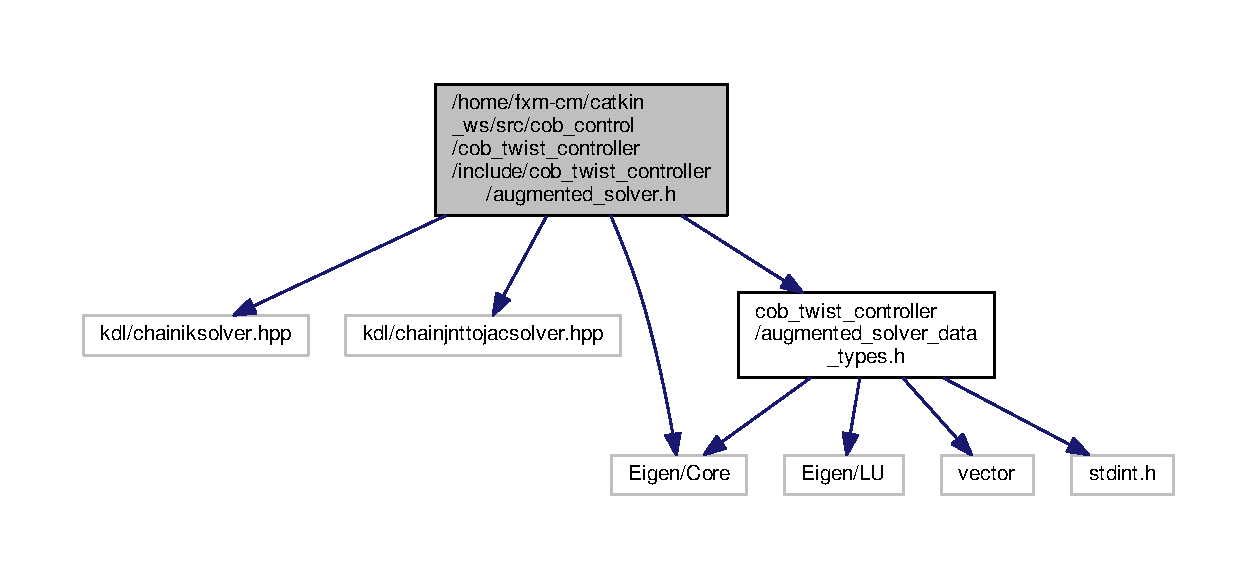
\includegraphics[width=350pt]{augmented__solver_8h__incl}
\end{center}
\end{figure}
This graph shows which files directly or indirectly include this file\-:
\nopagebreak
\begin{figure}[H]
\begin{center}
\leavevmode
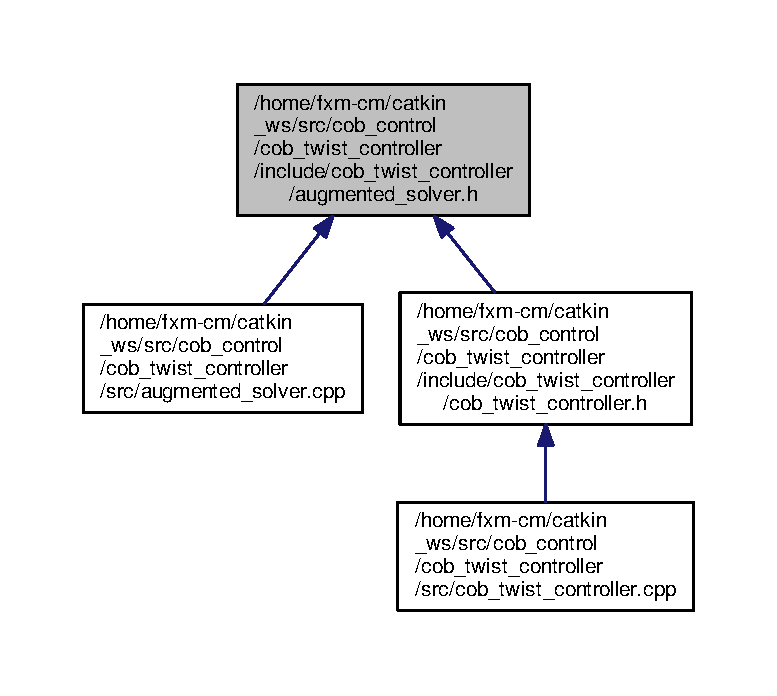
\includegraphics[width=350pt]{augmented__solver_8h__dep__incl}
\end{center}
\end{figure}
\subsection*{Classes}
\begin{DoxyCompactItemize}
\item 
class \hyperlink{classAugmentedSolver}{Augmented\-Solver}
\end{DoxyCompactItemize}


\subsection{Detailed Description}
This package provides the definitions of an inverse kinematics solver. \begin{DoxyNote}{Note}
Copyright (c) 2014 \par
 Fraunhofer Institute for Manufacturing Engineering and Automation (I\-P\-A) \par
\par


Project name\-: care-\/o-\/bot 

R\-O\-S stack name\-: cob\-\_\-control 

R\-O\-S package name\-: cob\-\_\-twist\-\_\-controller
\end{DoxyNote}
\begin{DoxyAuthor}{Author}
Author\-: Felix Messmer, email\-: \href{mailto:Felix.Messmer@ipa.fraunhofer.de}{\tt Felix.\-Messmer@ipa.\-fraunhofer.\-de}
\end{DoxyAuthor}
\begin{DoxyDate}{Date}
Date of creation\-: April, 2014 
\end{DoxyDate}

\hypertarget{augmented__solver__data__types_8h}{\section{/home/fxm-\/cm/catkin\-\_\-ws/src/cob\-\_\-control/cob\-\_\-twist\-\_\-controller/include/cob\-\_\-twist\-\_\-controller/augmented\-\_\-solver\-\_\-data\-\_\-types.h File Reference}
\label{augmented__solver__data__types_8h}\index{/home/fxm-\/cm/catkin\-\_\-ws/src/cob\-\_\-control/cob\-\_\-twist\-\_\-controller/include/cob\-\_\-twist\-\_\-controller/augmented\-\_\-solver\-\_\-data\-\_\-types.\-h@{/home/fxm-\/cm/catkin\-\_\-ws/src/cob\-\_\-control/cob\-\_\-twist\-\_\-controller/include/cob\-\_\-twist\-\_\-controller/augmented\-\_\-solver\-\_\-data\-\_\-types.\-h}}
}


Different data types for \hyperlink{classAugmentedSolver}{Augmented\-Solver} to be used in other modules.  


{\ttfamily \#include $<$Eigen/\-Core$>$}\\*
{\ttfamily \#include $<$Eigen/\-L\-U$>$}\\*
{\ttfamily \#include $<$vector$>$}\\*
{\ttfamily \#include $<$stdint.\-h$>$}\\*
Include dependency graph for augmented\-\_\-solver\-\_\-data\-\_\-types.\-h\-:
\nopagebreak
\begin{figure}[H]
\begin{center}
\leavevmode
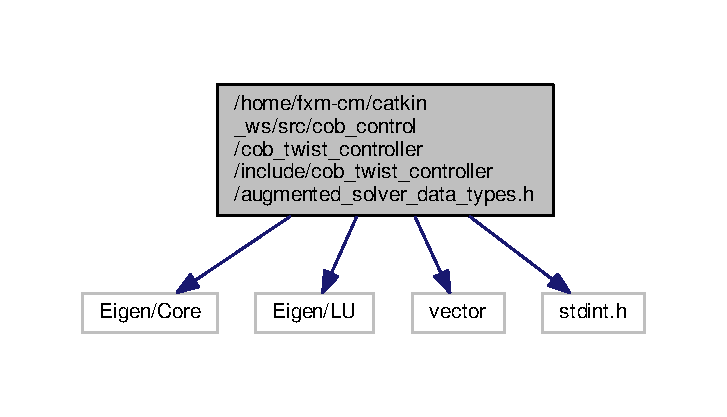
\includegraphics[width=349pt]{augmented__solver__data__types_8h__incl}
\end{center}
\end{figure}
This graph shows which files directly or indirectly include this file\-:
\nopagebreak
\begin{figure}[H]
\begin{center}
\leavevmode
\includegraphics[width=350pt]{augmented__solver__data__types_8h__dep__incl}
\end{center}
\end{figure}
\subsection*{Classes}
\begin{DoxyCompactItemize}
\item 
struct \hyperlink{structAugmentedSolverParams}{Augmented\-Solver\-Params}
\end{DoxyCompactItemize}
\subsection*{Typedefs}
\begin{DoxyCompactItemize}
\item 
\hypertarget{augmented__solver__data__types_8h_a81f3cefafed4e7b7a7d50c9bb411f5ef}{typedef Eigen\-::\-Matrix$<$ double, \\*
6, Eigen\-::\-Dynamic $>$ {\bfseries Matrix6\-Xd}}\label{augmented__solver__data__types_8h_a81f3cefafed4e7b7a7d50c9bb411f5ef}

\end{DoxyCompactItemize}
\subsection*{Enumerations}
\begin{DoxyCompactItemize}
\item 
enum {\bfseries Damping\-Method\-Types} \{ {\bfseries N\-O\-N\-E} = 0, 
{\bfseries C\-O\-N\-S\-T\-A\-N\-T} = 1, 
{\bfseries M\-A\-N\-I\-P\-U\-L\-A\-B\-I\-L\-I\-T\-Y} = 2
 \}
\item 
enum {\bfseries Contraint\-Types} \{ {\bfseries None} = 0, 
{\bfseries W\-L\-N} = 1, 
{\bfseries W\-L\-N\-\_\-\-J\-L\-A} = 2
 \}
\end{DoxyCompactItemize}


\subsection{Detailed Description}
Different data types for \hyperlink{classAugmentedSolver}{Augmented\-Solver} to be used in other modules. \begin{DoxyNote}{Note}
Copyright (c) 2015 \par
 Fraunhofer Institute for Manufacturing Engineering and Automation (I\-P\-A) \par
\par


Project name\-: care-\/o-\/bot 

R\-O\-S stack name\-: cob\-\_\-control 

R\-O\-S package name\-: cob\-\_\-twist\-\_\-controller
\end{DoxyNote}
\begin{DoxyAuthor}{Author}
Author\-: Marco Bezzon, email\-: \href{mailto:Marco.Bezzon@ipa.fraunhofer.de}{\tt Marco.\-Bezzon@ipa.\-fraunhofer.\-de}
\end{DoxyAuthor}
\begin{DoxyDate}{Date}
Date of creation\-: March, 2015 
\end{DoxyDate}

\hypertarget{cob__twist__controller_8h}{\section{/home/fxm-\/cm/catkin\-\_\-ws/src/cob\-\_\-control/cob\-\_\-twist\-\_\-controller/include/cob\-\_\-twist\-\_\-controller/cob\-\_\-twist\-\_\-controller.h File Reference}
\label{cob__twist__controller_8h}\index{/home/fxm-\/cm/catkin\-\_\-ws/src/cob\-\_\-control/cob\-\_\-twist\-\_\-controller/include/cob\-\_\-twist\-\_\-controller/cob\-\_\-twist\-\_\-controller.\-h@{/home/fxm-\/cm/catkin\-\_\-ws/src/cob\-\_\-control/cob\-\_\-twist\-\_\-controller/include/cob\-\_\-twist\-\_\-controller/cob\-\_\-twist\-\_\-controller.\-h}}
}


This package provides a generic Twist controller for the Care-\/\-O-\/bot.  


{\ttfamily \#include $<$ros/ros.\-h$>$}\\*
{\ttfamily \#include $<$std\-\_\-msgs/\-Float64.\-h$>$}\\*
{\ttfamily \#include $<$std\-\_\-msgs/\-Float64\-Multi\-Array.\-h$>$}\\*
{\ttfamily \#include $<$sensor\-\_\-msgs/\-Joint\-State.\-h$>$}\\*
{\ttfamily \#include $<$geometry\-\_\-msgs/\-Twist.\-h$>$}\\*
{\ttfamily \#include $<$nav\-\_\-msgs/\-Odometry.\-h$>$}\\*
{\ttfamily \#include $<$urdf/model.\-h$>$}\\*
{\ttfamily \#include $<$kdl\-\_\-parser/kdl\-\_\-parser.\-hpp$>$}\\*
{\ttfamily \#include $<$kdl/chainfksolvervel\-\_\-recursive.\-hpp$>$}\\*
{\ttfamily \#include $<$kdl/chainiksolvervel\-\_\-pinv.\-hpp$>$}\\*
{\ttfamily \#include $<$kdl/jntarray.\-hpp$>$}\\*
{\ttfamily \#include $<$kdl/jntarrayvel.\-hpp$>$}\\*
{\ttfamily \#include $<$kdl/frames.\-hpp$>$}\\*
{\ttfamily \#include $<$tf/transform\-\_\-listener.\-h$>$}\\*
{\ttfamily \#include $<$tf/tf.\-h$>$}\\*
{\ttfamily \#include $<$boost/thread/mutex.\-hpp$>$}\\*
{\ttfamily \#include $<$boost/shared\-\_\-ptr.\-hpp$>$}\\*
{\ttfamily \#include $<$dynamic\-\_\-reconfigure/server.\-h$>$}\\*
{\ttfamily \#include $<$cob\-\_\-twist\-\_\-controller/augmented\-\_\-solver.\-h$>$}\\*
{\ttfamily \#include $<$cob\-\_\-twist\-\_\-controller/\-Twist\-Controller\-Config.\-h$>$}\\*
{\ttfamily \#include \char`\"{}cob\-\_\-twist\-\_\-controller/cob\-\_\-twist\-\_\-controller\-\_\-data\-\_\-types.\-h\char`\"{}}\\*
{\ttfamily \#include \char`\"{}cob\-\_\-twist\-\_\-controller/limiters/limiter.\-h\char`\"{}}\\*
Include dependency graph for cob\-\_\-twist\-\_\-controller.\-h\-:
\nopagebreak
\begin{figure}[H]
\begin{center}
\leavevmode
\includegraphics[width=350pt]{cob__twist__controller_8h__incl}
\end{center}
\end{figure}
This graph shows which files directly or indirectly include this file\-:
\nopagebreak
\begin{figure}[H]
\begin{center}
\leavevmode
\includegraphics[width=222pt]{cob__twist__controller_8h__dep__incl}
\end{center}
\end{figure}
\subsection*{Classes}
\begin{DoxyCompactItemize}
\item 
class \hyperlink{classCobTwistController}{Cob\-Twist\-Controller}
\end{DoxyCompactItemize}


\subsection{Detailed Description}
This package provides a generic Twist controller for the Care-\/\-O-\/bot. \begin{DoxyNote}{Note}
Copyright (c) 2014 \par
 Fraunhofer Institute for Manufacturing Engineering and Automation (I\-P\-A) \par
\par


Project name\-: care-\/o-\/bot 

R\-O\-S stack name\-: cob\-\_\-driver 

R\-O\-S package name\-: cob\-\_\-twist\-\_\-controller
\end{DoxyNote}
\begin{DoxyAuthor}{Author}
Author\-: Felix Messmer, email\-: \href{mailto:Felix.Messmer@ipa.fraunhofer.de}{\tt Felix.\-Messmer@ipa.\-fraunhofer.\-de}
\end{DoxyAuthor}
\begin{DoxyDate}{Date}
Date of creation\-: April, 2014 
\end{DoxyDate}

\hypertarget{cob__twist__controller__data__types_8h}{\section{/home/fxm-\/cm/catkin\-\_\-ws/src/cob\-\_\-control/cob\-\_\-twist\-\_\-controller/include/cob\-\_\-twist\-\_\-controller/cob\-\_\-twist\-\_\-controller\-\_\-data\-\_\-types.h File Reference}
\label{cob__twist__controller__data__types_8h}\index{/home/fxm-\/cm/catkin\-\_\-ws/src/cob\-\_\-control/cob\-\_\-twist\-\_\-controller/include/cob\-\_\-twist\-\_\-controller/cob\-\_\-twist\-\_\-controller\-\_\-data\-\_\-types.\-h@{/home/fxm-\/cm/catkin\-\_\-ws/src/cob\-\_\-control/cob\-\_\-twist\-\_\-controller/include/cob\-\_\-twist\-\_\-controller/cob\-\_\-twist\-\_\-controller\-\_\-data\-\_\-types.\-h}}
}


Different data types for \hyperlink{classCobTwistController}{Cob\-Twist\-Controller} to be used in other modules.  


{\ttfamily \#include $<$vector$>$}\\*
{\ttfamily \#include $<$stdint.\-h$>$}\\*
Include dependency graph for cob\-\_\-twist\-\_\-controller\-\_\-data\-\_\-types.\-h\-:
\nopagebreak
\begin{figure}[H]
\begin{center}
\leavevmode
\includegraphics[width=246pt]{cob__twist__controller__data__types_8h__incl}
\end{center}
\end{figure}
This graph shows which files directly or indirectly include this file\-:
\nopagebreak
\begin{figure}[H]
\begin{center}
\leavevmode
\includegraphics[width=350pt]{cob__twist__controller__data__types_8h__dep__incl}
\end{center}
\end{figure}
\subsection*{Classes}
\begin{DoxyCompactItemize}
\item 
struct \hyperlink{structTwistControllerParams}{Twist\-Controller\-Params}
\end{DoxyCompactItemize}


\subsection{Detailed Description}
Different data types for \hyperlink{classCobTwistController}{Cob\-Twist\-Controller} to be used in other modules. \begin{DoxyNote}{Note}
Copyright (c) 2015 \par
 Fraunhofer Institute for Manufacturing Engineering and Automation (I\-P\-A) \par
\par


Project name\-: care-\/o-\/bot 

R\-O\-S stack name\-: cob\-\_\-control 

R\-O\-S package name\-: cob\-\_\-twist\-\_\-controller
\end{DoxyNote}
\begin{DoxyAuthor}{Author}
Author\-: Marco Bezzon, email\-: \href{mailto:Marco.Bezzon@ipa.fraunhofer.de}{\tt Marco.\-Bezzon@ipa.\-fraunhofer.\-de}
\end{DoxyAuthor}
\begin{DoxyDate}{Date}
Date of creation\-: April, 2015 
\end{DoxyDate}

\hypertarget{solver__factory_8h}{\section{/home/fxm-\/cm/catkin\-\_\-ws/src/cob\-\_\-control/cob\-\_\-twist\-\_\-controller/include/cob\-\_\-twist\-\_\-controller/constraint\-\_\-solvers/factories/solver\-\_\-factory.h File Reference}
\label{solver__factory_8h}\index{/home/fxm-\/cm/catkin\-\_\-ws/src/cob\-\_\-control/cob\-\_\-twist\-\_\-controller/include/cob\-\_\-twist\-\_\-controller/constraint\-\_\-solvers/factories/solver\-\_\-factory.\-h@{/home/fxm-\/cm/catkin\-\_\-ws/src/cob\-\_\-control/cob\-\_\-twist\-\_\-controller/include/cob\-\_\-twist\-\_\-controller/constraint\-\_\-solvers/factories/solver\-\_\-factory.\-h}}
}


This header contains the interface description to create solvers.  


{\ttfamily \#include $<$Eigen/\-Core$>$}\\*
{\ttfamily \#include $<$Eigen/\-S\-V\-D$>$}\\*
{\ttfamily \#include $<$kdl/jntarray.\-hpp$>$}\\*
Include dependency graph for solver\-\_\-factory.\-h\-:
\nopagebreak
\begin{figure}[H]
\begin{center}
\leavevmode
\includegraphics[width=328pt]{solver__factory_8h__incl}
\end{center}
\end{figure}
\subsection*{Classes}
\begin{DoxyCompactItemize}
\item 
class \hyperlink{classISolverFactory}{I\-Solver\-Factory}
\begin{DoxyCompactList}\small\item\em Interface definition to support generic usage of the solver factory without specifying a typename in prior. \end{DoxyCompactList}\item 
class \hyperlink{classSolverFactory}{Solver\-Factory$<$ T $>$}
\begin{DoxyCompactList}\small\item\em Abstract base class defining interfaces for the creation of a specific solver. \end{DoxyCompactList}\end{DoxyCompactItemize}


\subsection{Detailed Description}
This header contains the interface description to create solvers. \begin{DoxyNote}{Note}
Copyright (c) 2015 \par
 Fraunhofer Institute for Manufacturing Engineering and Automation (I\-P\-A) \par
\par


Project name\-: care-\/o-\/bot 

R\-O\-S stack name\-: cob\-\_\-control 

R\-O\-S package name\-: cob\-\_\-twist\-\_\-controller
\end{DoxyNote}
\begin{DoxyAuthor}{Author}
Author\-: Marco Bezzon, email\-: \href{mailto:Marco.Bezzon@ipa.fraunhofer.de}{\tt Marco.\-Bezzon@ipa.\-fraunhofer.\-de}
\end{DoxyAuthor}
\begin{DoxyDate}{Date}
Date of creation\-: March, 2015 
\end{DoxyDate}

\hypertarget{constraint__solver__base_8h}{\section{/home/fxm-\/cm/catkin\-\_\-ws/src/cob\-\_\-control/cob\-\_\-twist\-\_\-controller/include/cob\-\_\-twist\-\_\-controller/constraint\-\_\-solvers/solvers/constraint\-\_\-solver\-\_\-base.h File Reference}
\label{constraint__solver__base_8h}\index{/home/fxm-\/cm/catkin\-\_\-ws/src/cob\-\_\-control/cob\-\_\-twist\-\_\-controller/include/cob\-\_\-twist\-\_\-controller/constraint\-\_\-solvers/solvers/constraint\-\_\-solver\-\_\-base.\-h@{/home/fxm-\/cm/catkin\-\_\-ws/src/cob\-\_\-control/cob\-\_\-twist\-\_\-controller/include/cob\-\_\-twist\-\_\-controller/constraint\-\_\-solvers/solvers/constraint\-\_\-solver\-\_\-base.\-h}}
}


This header contains the interface description of constraint solvers Pure virtual methods have to be implemented in subclasses.  


{\ttfamily \#include $<$Eigen/\-Core$>$}\\*
{\ttfamily \#include $<$Eigen/\-S\-V\-D$>$}\\*
{\ttfamily \#include $<$kdl/jntarray.\-hpp$>$}\\*
{\ttfamily \#include \char`\"{}cob\-\_\-twist\-\_\-controller/augmented\-\_\-solver\-\_\-data\-\_\-types.\-h\char`\"{}}\\*
Include dependency graph for constraint\-\_\-solver\-\_\-base.\-h\-:
\nopagebreak
\begin{figure}[H]
\begin{center}
\leavevmode
\includegraphics[width=350pt]{constraint__solver__base_8h__incl}
\end{center}
\end{figure}
This graph shows which files directly or indirectly include this file\-:
\nopagebreak
\begin{figure}[H]
\begin{center}
\leavevmode
\includegraphics[width=350pt]{constraint__solver__base_8h__dep__incl}
\end{center}
\end{figure}
\subsection*{Classes}
\begin{DoxyCompactItemize}
\item 
class \hyperlink{classConstraintSolver}{Constraint\-Solver}
\begin{DoxyCompactList}\small\item\em Base class for solvers, defining interface methods. \end{DoxyCompactList}\end{DoxyCompactItemize}


\subsection{Detailed Description}
This header contains the interface description of constraint solvers Pure virtual methods have to be implemented in subclasses. \begin{DoxyNote}{Note}
Copyright (c) 2015 \par
 Fraunhofer Institute for Manufacturing Engineering and Automation (I\-P\-A) \par
\par


Project name\-: care-\/o-\/bot 

R\-O\-S stack name\-: cob\-\_\-control 

R\-O\-S package name\-: cob\-\_\-twist\-\_\-controller
\end{DoxyNote}
\begin{DoxyAuthor}{Author}
Author\-: Marco Bezzon, email\-: \href{mailto:Marco.Bezzon@ipa.fraunhofer.de}{\tt Marco.\-Bezzon@ipa.\-fraunhofer.\-de}
\end{DoxyAuthor}
\begin{DoxyDate}{Date}
Date of creation\-: March, 2015 
\end{DoxyDate}

\hypertarget{unconstraint__solver_8h}{\section{/home/fxm-\/cm/catkin\-\_\-ws/src/cob\-\_\-control/cob\-\_\-twist\-\_\-controller/include/cob\-\_\-twist\-\_\-controller/constraint\-\_\-solvers/solvers/unconstraint\-\_\-solver.h File Reference}
\label{unconstraint__solver_8h}\index{/home/fxm-\/cm/catkin\-\_\-ws/src/cob\-\_\-control/cob\-\_\-twist\-\_\-controller/include/cob\-\_\-twist\-\_\-controller/constraint\-\_\-solvers/solvers/unconstraint\-\_\-solver.\-h@{/home/fxm-\/cm/catkin\-\_\-ws/src/cob\-\_\-control/cob\-\_\-twist\-\_\-controller/include/cob\-\_\-twist\-\_\-controller/constraint\-\_\-solvers/solvers/unconstraint\-\_\-solver.\-h}}
}


This header contains the description of the unconstraint solver Implements methods from constraint\-\_\-solver\-\_\-base.  


{\ttfamily \#include \char`\"{}cob\-\_\-twist\-\_\-controller/augmented\-\_\-solver\-\_\-data\-\_\-types.\-h\char`\"{}}\\*
{\ttfamily \#include \char`\"{}cob\-\_\-twist\-\_\-controller/constraint\-\_\-solvers/solvers/constraint\-\_\-solver\-\_\-base.\-h\char`\"{}}\\*
Include dependency graph for unconstraint\-\_\-solver.\-h\-:
\nopagebreak
\begin{figure}[H]
\begin{center}
\leavevmode
\includegraphics[width=350pt]{unconstraint__solver_8h__incl}
\end{center}
\end{figure}
This graph shows which files directly or indirectly include this file\-:
\nopagebreak
\begin{figure}[H]
\begin{center}
\leavevmode
\includegraphics[width=236pt]{unconstraint__solver_8h__dep__incl}
\end{center}
\end{figure}
\subsection*{Classes}
\begin{DoxyCompactItemize}
\item 
class \hyperlink{classUnconstraintSolver}{Unconstraint\-Solver}
\end{DoxyCompactItemize}


\subsection{Detailed Description}
This header contains the description of the unconstraint solver Implements methods from constraint\-\_\-solver\-\_\-base. \begin{DoxyNote}{Note}
Copyright (c) 2015 \par
 Fraunhofer Institute for Manufacturing Engineering and Automation (I\-P\-A) \par
\par


Project name\-: care-\/o-\/bot 

R\-O\-S stack name\-: cob\-\_\-control 

R\-O\-S package name\-: cob\-\_\-twist\-\_\-controller
\end{DoxyNote}
\begin{DoxyAuthor}{Author}
Author\-: Marco Bezzon, email\-: \href{mailto:Marco.Bezzon@ipa.fraunhofer.de}{\tt Marco.\-Bezzon@ipa.\-fraunhofer.\-de}
\end{DoxyAuthor}
\begin{DoxyDate}{Date}
Date of creation\-: March, 2015 
\end{DoxyDate}

\hypertarget{weighted__least__norm__solver_8h}{\section{/home/fxm-\/cm/catkin\-\_\-ws/src/cob\-\_\-control/cob\-\_\-twist\-\_\-controller/include/cob\-\_\-twist\-\_\-controller/constraint\-\_\-solvers/solvers/weighted\-\_\-least\-\_\-norm\-\_\-solver.h File Reference}
\label{weighted__least__norm__solver_8h}\index{/home/fxm-\/cm/catkin\-\_\-ws/src/cob\-\_\-control/cob\-\_\-twist\-\_\-controller/include/cob\-\_\-twist\-\_\-controller/constraint\-\_\-solvers/solvers/weighted\-\_\-least\-\_\-norm\-\_\-solver.\-h@{/home/fxm-\/cm/catkin\-\_\-ws/src/cob\-\_\-control/cob\-\_\-twist\-\_\-controller/include/cob\-\_\-twist\-\_\-controller/constraint\-\_\-solvers/solvers/weighted\-\_\-least\-\_\-norm\-\_\-solver.\-h}}
}


This header contains the description of the J\-L\-A solver Implements methods from constraint\-\_\-solver\-\_\-base Special constraint handling.  


{\ttfamily \#include \char`\"{}cob\-\_\-twist\-\_\-controller/augmented\-\_\-solver\-\_\-data\-\_\-types.\-h\char`\"{}}\\*
{\ttfamily \#include \char`\"{}cob\-\_\-twist\-\_\-controller/constraint\-\_\-solvers/solvers/constraint\-\_\-solver\-\_\-base.\-h\char`\"{}}\\*
Include dependency graph for weighted\-\_\-least\-\_\-norm\-\_\-solver.\-h\-:
\nopagebreak
\begin{figure}[H]
\begin{center}
\leavevmode
\includegraphics[width=350pt]{weighted__least__norm__solver_8h__incl}
\end{center}
\end{figure}
This graph shows which files directly or indirectly include this file\-:
\nopagebreak
\begin{figure}[H]
\begin{center}
\leavevmode
\includegraphics[width=350pt]{weighted__least__norm__solver_8h__dep__incl}
\end{center}
\end{figure}
\subsection*{Classes}
\begin{DoxyCompactItemize}
\item 
class \hyperlink{classWeightedLeastNormSolver}{Weighted\-Least\-Norm\-Solver}
\begin{DoxyCompactList}\small\item\em Implementation of \hyperlink{classConstraintSolver}{Constraint\-Solver} to solve inverse kinematics by using a weighted least norm. \end{DoxyCompactList}\end{DoxyCompactItemize}


\subsection{Detailed Description}
This header contains the description of the J\-L\-A solver Implements methods from constraint\-\_\-solver\-\_\-base Special constraint handling. \begin{DoxyNote}{Note}
Copyright (c) 2015 \par
 Fraunhofer Institute for Manufacturing Engineering and Automation (I\-P\-A) \par
\par


Project name\-: care-\/o-\/bot 

R\-O\-S stack name\-: cob\-\_\-control 

R\-O\-S package name\-: cob\-\_\-twist\-\_\-controller
\end{DoxyNote}
\begin{DoxyAuthor}{Author}
Author\-: Marco Bezzon, email\-: \href{mailto:Marco.Bezzon@ipa.fraunhofer.de}{\tt Marco.\-Bezzon@ipa.\-fraunhofer.\-de}
\end{DoxyAuthor}
\begin{DoxyDate}{Date}
Date of creation\-: March, 2015 
\end{DoxyDate}

\hypertarget{wln__joint__limit__avoidance__solver_8h}{\section{/home/fxm-\/cm/catkin\-\_\-ws/src/cob\-\_\-control/cob\-\_\-twist\-\_\-controller/include/cob\-\_\-twist\-\_\-controller/constraint\-\_\-solvers/solvers/wln\-\_\-joint\-\_\-limit\-\_\-avoidance\-\_\-solver.h File Reference}
\label{wln__joint__limit__avoidance__solver_8h}\index{/home/fxm-\/cm/catkin\-\_\-ws/src/cob\-\_\-control/cob\-\_\-twist\-\_\-controller/include/cob\-\_\-twist\-\_\-controller/constraint\-\_\-solvers/solvers/wln\-\_\-joint\-\_\-limit\-\_\-avoidance\-\_\-solver.\-h@{/home/fxm-\/cm/catkin\-\_\-ws/src/cob\-\_\-control/cob\-\_\-twist\-\_\-controller/include/cob\-\_\-twist\-\_\-controller/constraint\-\_\-solvers/solvers/wln\-\_\-joint\-\_\-limit\-\_\-avoidance\-\_\-solver.\-h}}
}


This header contains the description of the J\-L\-A solver Implements methods from constraint\-\_\-solver\-\_\-base Special constraint handling.  


{\ttfamily \#include \char`\"{}cob\-\_\-twist\-\_\-controller/augmented\-\_\-solver\-\_\-data\-\_\-types.\-h\char`\"{}}\\*
{\ttfamily \#include \char`\"{}cob\-\_\-twist\-\_\-controller/constraint\-\_\-solvers/solvers/weighted\-\_\-least\-\_\-norm\-\_\-solver.\-h\char`\"{}}\\*
Include dependency graph for wln\-\_\-joint\-\_\-limit\-\_\-avoidance\-\_\-solver.\-h\-:
\nopagebreak
\begin{figure}[H]
\begin{center}
\leavevmode
\includegraphics[width=350pt]{wln__joint__limit__avoidance__solver_8h__incl}
\end{center}
\end{figure}
This graph shows which files directly or indirectly include this file\-:
\nopagebreak
\begin{figure}[H]
\begin{center}
\leavevmode
\includegraphics[width=250pt]{wln__joint__limit__avoidance__solver_8h__dep__incl}
\end{center}
\end{figure}
\subsection*{Classes}
\begin{DoxyCompactItemize}
\item 
class \hyperlink{classWLN__JointLimitAvoidanceSolver}{W\-L\-N\-\_\-\-Joint\-Limit\-Avoidance\-Solver}
\end{DoxyCompactItemize}


\subsection{Detailed Description}
This header contains the description of the J\-L\-A solver Implements methods from constraint\-\_\-solver\-\_\-base Special constraint handling. \begin{DoxyNote}{Note}
Copyright (c) 2015 \par
 Fraunhofer Institute for Manufacturing Engineering and Automation (I\-P\-A) \par
\par


Project name\-: care-\/o-\/bot 

R\-O\-S stack name\-: cob\-\_\-control 

R\-O\-S package name\-: cob\-\_\-twist\-\_\-controller
\end{DoxyNote}
\begin{DoxyAuthor}{Author}
Author\-: Marco Bezzon, email\-: \href{mailto:Marco.Bezzon@ipa.fraunhofer.de}{\tt Marco.\-Bezzon@ipa.\-fraunhofer.\-de}
\end{DoxyAuthor}
\begin{DoxyDate}{Date}
Date of creation\-: March, 2015 
\end{DoxyDate}

\hypertarget{damping_8h}{\section{/home/fxm-\/cm/catkin\-\_\-ws/src/cob\-\_\-control/cob\-\_\-twist\-\_\-controller/include/cob\-\_\-twist\-\_\-controller/damping\-\_\-methods/damping.h File Reference}
\label{damping_8h}\index{/home/fxm-\/cm/catkin\-\_\-ws/src/cob\-\_\-control/cob\-\_\-twist\-\_\-controller/include/cob\-\_\-twist\-\_\-controller/damping\-\_\-methods/damping.\-h@{/home/fxm-\/cm/catkin\-\_\-ws/src/cob\-\_\-control/cob\-\_\-twist\-\_\-controller/include/cob\-\_\-twist\-\_\-controller/damping\-\_\-methods/damping.\-h}}
}


This header contains the class and method definitions of several damping methods.  


{\ttfamily \#include \char`\"{}cob\-\_\-twist\-\_\-controller/damping\-\_\-methods/damping\-\_\-base.\-h\char`\"{}}\\*
Include dependency graph for damping.\-h\-:
\nopagebreak
\begin{figure}[H]
\begin{center}
\leavevmode
\includegraphics[width=349pt]{damping_8h__incl}
\end{center}
\end{figure}
This graph shows which files directly or indirectly include this file\-:
\nopagebreak
\begin{figure}[H]
\begin{center}
\leavevmode
\includegraphics[width=254pt]{damping_8h__dep__incl}
\end{center}
\end{figure}
\subsection*{Classes}
\begin{DoxyCompactItemize}
\item 
class \hyperlink{classDampingBuilder}{Damping\-Builder}
\begin{DoxyCompactList}\small\item\em Class providing a static method to create damping method objects. \end{DoxyCompactList}\item 
class \hyperlink{classDampingNone}{Damping\-None}
\begin{DoxyCompactList}\small\item\em Class implementing a method to return the constant factor. \end{DoxyCompactList}\item 
class \hyperlink{classDampingConstant}{Damping\-Constant}
\begin{DoxyCompactList}\small\item\em Class implementing a method to return the constant factor. \end{DoxyCompactList}\item 
class \hyperlink{classDampingManipulability}{Damping\-Manipulability}
\begin{DoxyCompactList}\small\item\em Class implementing a method to return a factor corresponding to the measure of manipulability. \end{DoxyCompactList}\end{DoxyCompactItemize}


\subsection{Detailed Description}
This header contains the class and method definitions of several damping methods. \begin{DoxyNote}{Note}
Copyright (c) 2015 \par
 Fraunhofer Institute for Manufacturing Engineering and Automation (I\-P\-A) \par
\par


Project name\-: care-\/o-\/bot 

R\-O\-S stack name\-: cob\-\_\-control 

R\-O\-S package name\-: cob\-\_\-twist\-\_\-controller
\end{DoxyNote}
\begin{DoxyAuthor}{Author}
Author\-: Marco Bezzon, email\-: \href{mailto:Marco.Bezzon@ipa.fraunhofer.de}{\tt Marco.\-Bezzon@ipa.\-fraunhofer.\-de}
\end{DoxyAuthor}
\begin{DoxyDate}{Date}
Date of creation\-: March, 2015 
\end{DoxyDate}

\hypertarget{damping__base_8h}{\section{/home/fxm-\/cm/catkin\-\_\-ws/src/cob\-\_\-control/cob\-\_\-twist\-\_\-controller/include/cob\-\_\-twist\-\_\-controller/damping\-\_\-methods/damping\-\_\-base.h File Reference}
\label{damping__base_8h}\index{/home/fxm-\/cm/catkin\-\_\-ws/src/cob\-\_\-control/cob\-\_\-twist\-\_\-controller/include/cob\-\_\-twist\-\_\-controller/damping\-\_\-methods/damping\-\_\-base.\-h@{/home/fxm-\/cm/catkin\-\_\-ws/src/cob\-\_\-control/cob\-\_\-twist\-\_\-controller/include/cob\-\_\-twist\-\_\-controller/damping\-\_\-methods/damping\-\_\-base.\-h}}
}


This header contains the interface description of damping methods.  


{\ttfamily \#include \char`\"{}cob\-\_\-twist\-\_\-controller/augmented\-\_\-solver\-\_\-data\-\_\-types.\-h\char`\"{}}\\*
Include dependency graph for damping\-\_\-base.\-h\-:
\nopagebreak
\begin{figure}[H]
\begin{center}
\leavevmode
\includegraphics[width=349pt]{damping__base_8h__incl}
\end{center}
\end{figure}
This graph shows which files directly or indirectly include this file\-:
\nopagebreak
\begin{figure}[H]
\begin{center}
\leavevmode
\includegraphics[width=350pt]{damping__base_8h__dep__incl}
\end{center}
\end{figure}
\subsection*{Classes}
\begin{DoxyCompactItemize}
\item 
class \hyperlink{classDampingBase}{Damping\-Base}
\begin{DoxyCompactList}\small\item\em Base class for solvers, defining interface methods. \end{DoxyCompactList}\end{DoxyCompactItemize}


\subsection{Detailed Description}
This header contains the interface description of damping methods. \begin{DoxyNote}{Note}
Copyright (c) 2015 \par
 Fraunhofer Institute for Manufacturing Engineering and Automation (I\-P\-A) \par
\par


Project name\-: care-\/o-\/bot 

R\-O\-S stack name\-: cob\-\_\-control 

R\-O\-S package name\-: cob\-\_\-twist\-\_\-controller
\end{DoxyNote}
\begin{DoxyAuthor}{Author}
Author\-: Marco Bezzon, email\-: \href{mailto:Marco.Bezzon@ipa.fraunhofer.de}{\tt Marco.\-Bezzon@ipa.\-fraunhofer.\-de}
\end{DoxyAuthor}
\begin{DoxyDate}{Date}
Date of creation\-: March, 2015 
\end{DoxyDate}

\hypertarget{limiter_8h}{\section{/home/fxm-\/cm/catkin\-\_\-ws/src/cob\-\_\-control/cob\-\_\-twist\-\_\-controller/include/cob\-\_\-twist\-\_\-controller/limiters/limiter.h File Reference}
\label{limiter_8h}\index{/home/fxm-\/cm/catkin\-\_\-ws/src/cob\-\_\-control/cob\-\_\-twist\-\_\-controller/include/cob\-\_\-twist\-\_\-controller/limiters/limiter.\-h@{/home/fxm-\/cm/catkin\-\_\-ws/src/cob\-\_\-control/cob\-\_\-twist\-\_\-controller/include/cob\-\_\-twist\-\_\-controller/limiters/limiter.\-h}}
}


This header contains the class definitions of all limiter implementations.  


{\ttfamily \#include \char`\"{}cob\-\_\-twist\-\_\-controller/limiters/limiter\-\_\-base.\-h\char`\"{}}\\*
{\ttfamily \#include $<$vector$>$}\\*
Include dependency graph for limiter.\-h\-:
\nopagebreak
\begin{figure}[H]
\begin{center}
\leavevmode
\includegraphics[width=350pt]{limiter_8h__incl}
\end{center}
\end{figure}
This graph shows which files directly or indirectly include this file\-:
\nopagebreak
\begin{figure}[H]
\begin{center}
\leavevmode
\includegraphics[width=350pt]{limiter_8h__dep__incl}
\end{center}
\end{figure}
\subsection*{Classes}
\begin{DoxyCompactItemize}
\item 
class \hyperlink{classLimiterContainer}{Limiter\-Container}
\begin{DoxyCompactList}\small\item\em Container for limiters, implementing interface methods. \end{DoxyCompactList}\item 
class \hyperlink{classLimiterAllJointPositions}{Limiter\-All\-Joint\-Positions}
\begin{DoxyCompactList}\small\item\em Class for limiters, declaring the method to limit all joint positions. \end{DoxyCompactList}\item 
class \hyperlink{classLimiterAllJointVelocities}{Limiter\-All\-Joint\-Velocities}
\begin{DoxyCompactList}\small\item\em Class for joint velocity limiter (all scaled to keep direction), implementing interface methods. \end{DoxyCompactList}\item 
class \hyperlink{classLimiterIndividualJointPositions}{Limiter\-Individual\-Joint\-Positions}
\begin{DoxyCompactList}\small\item\em Class for a limiter, declaring a method to limit joint positions individually. \end{DoxyCompactList}\item 
class \hyperlink{classLimiterIndividualJointVelocities}{Limiter\-Individual\-Joint\-Velocities}
\begin{DoxyCompactList}\small\item\em Class for joint velocity limiter (individually scaled -\/$>$ changes direction), implementing interface methods. \end{DoxyCompactList}\end{DoxyCompactItemize}


\subsection{Detailed Description}
This header contains the class definitions of all limiter implementations. \begin{DoxyNote}{Note}
Copyright (c) 2015 \par
 Fraunhofer Institute for Manufacturing Engineering and Automation (I\-P\-A) \par
\par


Project name\-: care-\/o-\/bot 

R\-O\-S stack name\-: cob\-\_\-control 

R\-O\-S package name\-: cob\-\_\-twist\-\_\-controller
\end{DoxyNote}
\begin{DoxyAuthor}{Author}
Author\-: Marco Bezzon, email\-: \href{mailto:Marco.Bezzon@ipa.fraunhofer.de}{\tt Marco.\-Bezzon@ipa.\-fraunhofer.\-de}
\end{DoxyAuthor}
\begin{DoxyDate}{Date}
Date of creation\-: April, 2015 
\end{DoxyDate}

\hypertarget{limiter__base_8h}{\section{/home/fxm-\/cm/catkin\-\_\-ws/src/cob\-\_\-control/cob\-\_\-twist\-\_\-controller/include/cob\-\_\-twist\-\_\-controller/limiters/limiter\-\_\-base.h File Reference}
\label{limiter__base_8h}\index{/home/fxm-\/cm/catkin\-\_\-ws/src/cob\-\_\-control/cob\-\_\-twist\-\_\-controller/include/cob\-\_\-twist\-\_\-controller/limiters/limiter\-\_\-base.\-h@{/home/fxm-\/cm/catkin\-\_\-ws/src/cob\-\_\-control/cob\-\_\-twist\-\_\-controller/include/cob\-\_\-twist\-\_\-controller/limiters/limiter\-\_\-base.\-h}}
}


This header contains the interface description of limiters.  


{\ttfamily \#include \char`\"{}cob\-\_\-twist\-\_\-controller/cob\-\_\-twist\-\_\-controller\-\_\-data\-\_\-types.\-h\char`\"{}}\\*
{\ttfamily \#include $<$kdl/chain.\-hpp$>$}\\*
{\ttfamily \#include $<$kdl/chainiksolver.\-hpp$>$}\\*
{\ttfamily \#include $<$kdl/chainjnttojacsolver.\-hpp$>$}\\*
Include dependency graph for limiter\-\_\-base.\-h\-:
\nopagebreak
\begin{figure}[H]
\begin{center}
\leavevmode
\includegraphics[width=350pt]{limiter__base_8h__incl}
\end{center}
\end{figure}
This graph shows which files directly or indirectly include this file\-:
\nopagebreak
\begin{figure}[H]
\begin{center}
\leavevmode
\includegraphics[width=350pt]{limiter__base_8h__dep__incl}
\end{center}
\end{figure}
\subsection*{Classes}
\begin{DoxyCompactItemize}
\item 
class \hyperlink{classLimiterBase}{Limiter\-Base}
\begin{DoxyCompactList}\small\item\em Base class for limiters, defining interface methods. \end{DoxyCompactList}\end{DoxyCompactItemize}


\subsection{Detailed Description}
This header contains the interface description of limiters. \begin{DoxyNote}{Note}
Copyright (c) 2015 \par
 Fraunhofer Institute for Manufacturing Engineering and Automation (I\-P\-A) \par
\par


Project name\-: care-\/o-\/bot 

R\-O\-S stack name\-: cob\-\_\-control 

R\-O\-S package name\-: cob\-\_\-twist\-\_\-controller
\end{DoxyNote}
\begin{DoxyAuthor}{Author}
Author\-: Marco Bezzon, email\-: \href{mailto:Marco.Bezzon@ipa.fraunhofer.de}{\tt Marco.\-Bezzon@ipa.\-fraunhofer.\-de}
\end{DoxyAuthor}
\begin{DoxyDate}{Date}
Date of creation\-: April, 2015 
\end{DoxyDate}

\hypertarget{augmented__solver_8cpp}{\section{/home/fxm-\/cm/catkin\-\_\-ws/src/cob\-\_\-control/cob\-\_\-twist\-\_\-controller/src/augmented\-\_\-solver.cpp File Reference}
\label{augmented__solver_8cpp}\index{/home/fxm-\/cm/catkin\-\_\-ws/src/cob\-\_\-control/cob\-\_\-twist\-\_\-controller/src/augmented\-\_\-solver.\-cpp@{/home/fxm-\/cm/catkin\-\_\-ws/src/cob\-\_\-control/cob\-\_\-twist\-\_\-controller/src/augmented\-\_\-solver.\-cpp}}
}


This package provides the implementation of an inverse kinematics solver.  


{\ttfamily \#include \char`\"{}cob\-\_\-twist\-\_\-controller/augmented\-\_\-solver.\-h\char`\"{}}\\*
{\ttfamily \#include \char`\"{}cob\-\_\-twist\-\_\-controller/constraint\-\_\-solvers/constraint\-\_\-solver\-\_\-factory\-\_\-builder.\-h\char`\"{}}\\*
Include dependency graph for augmented\-\_\-solver.\-cpp\-:
\nopagebreak
\begin{figure}[H]
\begin{center}
\leavevmode
\includegraphics[width=350pt]{augmented__solver_8cpp__incl}
\end{center}
\end{figure}


\subsection{Detailed Description}
This package provides the implementation of an inverse kinematics solver. \begin{DoxyNote}{Note}
Copyright (c) 2014 \par
 Fraunhofer Institute for Manufacturing Engineering and Automation (I\-P\-A) \par
\par


Project name\-: care-\/o-\/bot 

R\-O\-S stack name\-: cob\-\_\-control 

R\-O\-S package name\-: cob\-\_\-twist\-\_\-controller
\end{DoxyNote}
\begin{DoxyAuthor}{Author}
Author\-: Felix Messmer, email\-: \href{mailto:Felix.Messmer@ipa.fraunhofer.de}{\tt Felix.\-Messmer@ipa.\-fraunhofer.\-de}
\end{DoxyAuthor}
\begin{DoxyDate}{Date}
Date of creation\-: April, 2014 
\end{DoxyDate}

\hypertarget{cob__twist__controller_8cpp}{\section{/home/fxm-\/cm/catkin\-\_\-ws/src/cob\-\_\-control/cob\-\_\-twist\-\_\-controller/src/cob\-\_\-twist\-\_\-controller.cpp File Reference}
\label{cob__twist__controller_8cpp}\index{/home/fxm-\/cm/catkin\-\_\-ws/src/cob\-\_\-control/cob\-\_\-twist\-\_\-controller/src/cob\-\_\-twist\-\_\-controller.\-cpp@{/home/fxm-\/cm/catkin\-\_\-ws/src/cob\-\_\-control/cob\-\_\-twist\-\_\-controller/src/cob\-\_\-twist\-\_\-controller.\-cpp}}
}


This package provides a generic Twist controller for the Care-\/\-O-\/bot.  


{\ttfamily \#include $<$ros/ros.\-h$>$}\\*
{\ttfamily \#include $<$cob\-\_\-twist\-\_\-controller/cob\-\_\-twist\-\_\-controller.\-h$>$}\\*
{\ttfamily \#include $<$kdl\-\_\-conversions/kdl\-\_\-msg.\-h$>$}\\*
{\ttfamily \#include $<$tf/transform\-\_\-datatypes.\-h$>$}\\*
{\ttfamily \#include $<$visualization\-\_\-msgs/\-Marker.\-h$>$}\\*
{\ttfamily \#include $<$Eigen/\-Dense$>$}\\*
Include dependency graph for cob\-\_\-twist\-\_\-controller.\-cpp\-:
\nopagebreak
\begin{figure}[H]
\begin{center}
\leavevmode
\includegraphics[width=350pt]{cob__twist__controller_8cpp__incl}
\end{center}
\end{figure}
\subsection*{Macros}
\begin{DoxyCompactItemize}
\item 
\hypertarget{cob__twist__controller_8cpp_ad24f6358a8505b74421d1eacc5155dc5}{\#define {\bfseries D\-E\-B\-U\-G\-\_\-\-B\-A\-S\-E\-\_\-\-A\-C\-T\-I\-V\-E}~0}\label{cob__twist__controller_8cpp_ad24f6358a8505b74421d1eacc5155dc5}

\item 
\hypertarget{cob__twist__controller_8cpp_a87a019c851743fdc7e4b034cf81cf757}{\#define {\bfseries D\-E\-B\-U\-G\-\_\-\-B\-A\-S\-E\-\_\-\-C\-O\-M\-P}~0}\label{cob__twist__controller_8cpp_a87a019c851743fdc7e4b034cf81cf757}

\end{DoxyCompactItemize}


\subsection{Detailed Description}
This package provides a generic Twist controller for the Care-\/\-O-\/bot. \begin{DoxyNote}{Note}
Copyright (c) 2014 \par
 Fraunhofer Institute for Manufacturing Engineering and Automation (I\-P\-A) \par
\par


Project name\-: care-\/o-\/bot 

R\-O\-S stack name\-: cob\-\_\-control 

R\-O\-S package name\-: cob\-\_\-twist\-\_\-controller
\end{DoxyNote}
\begin{DoxyAuthor}{Author}
Author\-: Felix Messmer, email\-: \href{mailto:Felix.Messmer@ipa.fraunhofer.de}{\tt Felix.\-Messmer@ipa.\-fraunhofer.\-de}
\end{DoxyAuthor}
\begin{DoxyDate}{Date}
Date of creation\-: April, 2014 
\end{DoxyDate}

\hypertarget{constraint__solver__base_8cpp}{\section{/home/fxm-\/cm/catkin\-\_\-ws/src/cob\-\_\-control/cob\-\_\-twist\-\_\-controller/src/constraint\-\_\-solvers/solvers/constraint\-\_\-solver\-\_\-base.cpp File Reference}
\label{constraint__solver__base_8cpp}\index{/home/fxm-\/cm/catkin\-\_\-ws/src/cob\-\_\-control/cob\-\_\-twist\-\_\-controller/src/constraint\-\_\-solvers/solvers/constraint\-\_\-solver\-\_\-base.\-cpp@{/home/fxm-\/cm/catkin\-\_\-ws/src/cob\-\_\-control/cob\-\_\-twist\-\_\-controller/src/constraint\-\_\-solvers/solvers/constraint\-\_\-solver\-\_\-base.\-cpp}}
}


Implementation of constructor for constraint\-\_\-solver\-\_\-base.  


{\ttfamily \#include \char`\"{}ros/ros.\-h\char`\"{}}\\*
{\ttfamily \#include \char`\"{}cob\-\_\-twist\-\_\-controller/constraint\-\_\-solvers/solvers/constraint\-\_\-solver\-\_\-base.\-h\char`\"{}}\\*
Include dependency graph for constraint\-\_\-solver\-\_\-base.\-cpp\-:
\nopagebreak
\begin{figure}[H]
\begin{center}
\leavevmode
\includegraphics[width=350pt]{constraint__solver__base_8cpp__incl}
\end{center}
\end{figure}


\subsection{Detailed Description}
Implementation of constructor for constraint\-\_\-solver\-\_\-base. \begin{DoxyNote}{Note}
Copyright (c) 2015 \par
 Fraunhofer Institute for Manufacturing Engineering and Automation (I\-P\-A) \par
\par


Project name\-: care-\/o-\/bot 

R\-O\-S stack name\-: cob\-\_\-control 

R\-O\-S package name\-: cob\-\_\-twist\-\_\-controller
\end{DoxyNote}
\begin{DoxyAuthor}{Author}
Author\-: Marco Bezzon, email\-: \href{mailto:Marco.Bezzon@ipa.fraunhofer.de}{\tt Marco.\-Bezzon@ipa.\-fraunhofer.\-de}
\end{DoxyAuthor}
\begin{DoxyDate}{Date}
Date of creation\-: March, 2015 
\end{DoxyDate}

\hypertarget{unconstraint__solver_8cpp}{\section{/home/fxm-\/cm/catkin\-\_\-ws/src/cob\-\_\-control/cob\-\_\-twist\-\_\-controller/src/constraint\-\_\-solvers/solvers/unconstraint\-\_\-solver.cpp File Reference}
\label{unconstraint__solver_8cpp}\index{/home/fxm-\/cm/catkin\-\_\-ws/src/cob\-\_\-control/cob\-\_\-twist\-\_\-controller/src/constraint\-\_\-solvers/solvers/unconstraint\-\_\-solver.\-cpp@{/home/fxm-\/cm/catkin\-\_\-ws/src/cob\-\_\-control/cob\-\_\-twist\-\_\-controller/src/constraint\-\_\-solvers/solvers/unconstraint\-\_\-solver.\-cpp}}
}


Implementation of an unconstraint solver.  


{\ttfamily \#include \char`\"{}cob\-\_\-twist\-\_\-controller/constraint\-\_\-solvers/solvers/unconstraint\-\_\-solver.\-h\char`\"{}}\\*
Include dependency graph for unconstraint\-\_\-solver.\-cpp\-:
\nopagebreak
\begin{figure}[H]
\begin{center}
\leavevmode
\includegraphics[width=350pt]{unconstraint__solver_8cpp__incl}
\end{center}
\end{figure}


\subsection{Detailed Description}
Implementation of an unconstraint solver. \begin{DoxyNote}{Note}
Copyright (c) 2015 \par
 Fraunhofer Institute for Manufacturing Engineering and Automation (I\-P\-A) \par
\par


Project name\-: care-\/o-\/bot 

R\-O\-S stack name\-: cob\-\_\-control 

R\-O\-S package name\-: cob\-\_\-twist\-\_\-controller
\end{DoxyNote}
\begin{DoxyAuthor}{Author}
Author\-: Marco Bezzon, email\-: \href{mailto:Marco.Bezzon@ipa.fraunhofer.de}{\tt Marco.\-Bezzon@ipa.\-fraunhofer.\-de}
\end{DoxyAuthor}
\begin{DoxyDate}{Date}
Date of creation\-: March, 2015 
\end{DoxyDate}

\hypertarget{weighted__least__norm__solver_8cpp}{\section{/home/fxm-\/cm/catkin\-\_\-ws/src/cob\-\_\-control/cob\-\_\-twist\-\_\-controller/src/constraint\-\_\-solvers/solvers/weighted\-\_\-least\-\_\-norm\-\_\-solver.cpp File Reference}
\label{weighted__least__norm__solver_8cpp}\index{/home/fxm-\/cm/catkin\-\_\-ws/src/cob\-\_\-control/cob\-\_\-twist\-\_\-controller/src/constraint\-\_\-solvers/solvers/weighted\-\_\-least\-\_\-norm\-\_\-solver.\-cpp@{/home/fxm-\/cm/catkin\-\_\-ws/src/cob\-\_\-control/cob\-\_\-twist\-\_\-controller/src/constraint\-\_\-solvers/solvers/weighted\-\_\-least\-\_\-norm\-\_\-solver.\-cpp}}
}


Implementation of an J\-L\-A solver. Special constraint\-: Avoid joint limits.  


{\ttfamily \#include \char`\"{}ros/ros.\-h\char`\"{}}\\*
{\ttfamily \#include \char`\"{}cob\-\_\-twist\-\_\-controller/constraint\-\_\-solvers/solvers/weighted\-\_\-least\-\_\-norm\-\_\-solver.\-h\char`\"{}}\\*
Include dependency graph for weighted\-\_\-least\-\_\-norm\-\_\-solver.\-cpp\-:
\nopagebreak
\begin{figure}[H]
\begin{center}
\leavevmode
\includegraphics[width=350pt]{weighted__least__norm__solver_8cpp__incl}
\end{center}
\end{figure}


\subsection{Detailed Description}
Implementation of an J\-L\-A solver. Special constraint\-: Avoid joint limits. \begin{DoxyNote}{Note}
Copyright (c) 2015 \par
 Fraunhofer Institute for Manufacturing Engineering and Automation (I\-P\-A) \par
\par


Project name\-: care-\/o-\/bot 

R\-O\-S stack name\-: cob\-\_\-control 

R\-O\-S package name\-: cob\-\_\-twist\-\_\-controller
\end{DoxyNote}
\begin{DoxyAuthor}{Author}
Author\-: Marco Bezzon, email\-: \href{mailto:Marco.Bezzon@ipa.fraunhofer.de}{\tt Marco.\-Bezzon@ipa.\-fraunhofer.\-de}
\end{DoxyAuthor}
\begin{DoxyDate}{Date}
Date of creation\-: March, 2015 
\end{DoxyDate}

\hypertarget{wln__joint__limit__avoidance__solver_8cpp}{\section{/home/fxm-\/cm/catkin\-\_\-ws/src/cob\-\_\-control/cob\-\_\-twist\-\_\-controller/src/constraint\-\_\-solvers/solvers/wln\-\_\-joint\-\_\-limit\-\_\-avoidance\-\_\-solver.cpp File Reference}
\label{wln__joint__limit__avoidance__solver_8cpp}\index{/home/fxm-\/cm/catkin\-\_\-ws/src/cob\-\_\-control/cob\-\_\-twist\-\_\-controller/src/constraint\-\_\-solvers/solvers/wln\-\_\-joint\-\_\-limit\-\_\-avoidance\-\_\-solver.\-cpp@{/home/fxm-\/cm/catkin\-\_\-ws/src/cob\-\_\-control/cob\-\_\-twist\-\_\-controller/src/constraint\-\_\-solvers/solvers/wln\-\_\-joint\-\_\-limit\-\_\-avoidance\-\_\-solver.\-cpp}}
}


Implementation of an J\-L\-A solver. Special constraint\-: Avoid joint limits.  


{\ttfamily \#include \char`\"{}cob\-\_\-twist\-\_\-controller/constraint\-\_\-solvers/solvers/wln\-\_\-joint\-\_\-limit\-\_\-avoidance\-\_\-solver.\-h\char`\"{}}\\*
Include dependency graph for wln\-\_\-joint\-\_\-limit\-\_\-avoidance\-\_\-solver.\-cpp\-:
\nopagebreak
\begin{figure}[H]
\begin{center}
\leavevmode
\includegraphics[width=350pt]{wln__joint__limit__avoidance__solver_8cpp__incl}
\end{center}
\end{figure}


\subsection{Detailed Description}
Implementation of an J\-L\-A solver. Special constraint\-: Avoid joint limits. \begin{DoxyNote}{Note}
Copyright (c) 2015 \par
 Fraunhofer Institute for Manufacturing Engineering and Automation (I\-P\-A) \par
\par


Project name\-: care-\/o-\/bot 

R\-O\-S stack name\-: cob\-\_\-control 

R\-O\-S package name\-: cob\-\_\-twist\-\_\-controller
\end{DoxyNote}
\begin{DoxyAuthor}{Author}
Author\-: Marco Bezzon, email\-: \href{mailto:Marco.Bezzon@ipa.fraunhofer.de}{\tt Marco.\-Bezzon@ipa.\-fraunhofer.\-de}
\end{DoxyAuthor}
\begin{DoxyDate}{Date}
Date of creation\-: March, 2015 
\end{DoxyDate}

\hypertarget{damping_8cpp}{\section{/home/fxm-\/cm/catkin\-\_\-ws/src/cob\-\_\-control/cob\-\_\-twist\-\_\-controller/src/damping\-\_\-methods/damping.cpp File Reference}
\label{damping_8cpp}\index{/home/fxm-\/cm/catkin\-\_\-ws/src/cob\-\_\-control/cob\-\_\-twist\-\_\-controller/src/damping\-\_\-methods/damping.\-cpp@{/home/fxm-\/cm/catkin\-\_\-ws/src/cob\-\_\-control/cob\-\_\-twist\-\_\-controller/src/damping\-\_\-methods/damping.\-cpp}}
}


This module contains the implementation of all available damping methods.  


{\ttfamily \#include \char`\"{}ros/ros.\-h\char`\"{}}\\*
{\ttfamily \#include \char`\"{}cob\-\_\-twist\-\_\-controller/damping\-\_\-methods/damping.\-h\char`\"{}}\\*
Include dependency graph for damping.\-cpp\-:
\nopagebreak
\begin{figure}[H]
\begin{center}
\leavevmode
\includegraphics[width=350pt]{damping_8cpp__incl}
\end{center}
\end{figure}


\subsection{Detailed Description}
This module contains the implementation of all available damping methods. \begin{DoxyNote}{Note}
Copyright (c) 2015 \par
 Fraunhofer Institute for Manufacturing Engineering and Automation (I\-P\-A) \par
\par


Project name\-: care-\/o-\/bot 

R\-O\-S stack name\-: cob\-\_\-control 

R\-O\-S package name\-: cob\-\_\-twist\-\_\-controller
\end{DoxyNote}
\begin{DoxyAuthor}{Author}
Author\-: Marco Bezzon, email\-: \href{mailto:Marco.Bezzon@ipa.fraunhofer.de}{\tt Marco.\-Bezzon@ipa.\-fraunhofer.\-de}
\end{DoxyAuthor}
\begin{DoxyDate}{Date}
Date of creation\-: March, 2015 
\end{DoxyDate}

\hypertarget{damping__base_8cpp}{\section{/home/fxm-\/cm/catkin\-\_\-ws/src/cob\-\_\-control/cob\-\_\-twist\-\_\-controller/src/damping\-\_\-methods/damping\-\_\-base.cpp File Reference}
\label{damping__base_8cpp}\index{/home/fxm-\/cm/catkin\-\_\-ws/src/cob\-\_\-control/cob\-\_\-twist\-\_\-controller/src/damping\-\_\-methods/damping\-\_\-base.\-cpp@{/home/fxm-\/cm/catkin\-\_\-ws/src/cob\-\_\-control/cob\-\_\-twist\-\_\-controller/src/damping\-\_\-methods/damping\-\_\-base.\-cpp}}
}


This header contains the interface description of damping methods.  


{\ttfamily \#include \char`\"{}cob\-\_\-twist\-\_\-controller/damping\-\_\-methods/damping\-\_\-base.\-h\char`\"{}}\\*
Include dependency graph for damping\-\_\-base.\-cpp\-:
\nopagebreak
\begin{figure}[H]
\begin{center}
\leavevmode
\includegraphics[width=349pt]{damping__base_8cpp__incl}
\end{center}
\end{figure}


\subsection{Detailed Description}
This header contains the interface description of damping methods. \begin{DoxyNote}{Note}
Copyright (c) 2015 \par
 Fraunhofer Institute for Manufacturing Engineering and Automation (I\-P\-A) \par
\par


Project name\-: care-\/o-\/bot 

R\-O\-S stack name\-: cob\-\_\-control 

R\-O\-S package name\-: cob\-\_\-twist\-\_\-controller
\end{DoxyNote}
\begin{DoxyAuthor}{Author}
Author\-: Marco Bezzon, email\-: \href{mailto:Marco.Bezzon@ipa.fraunhofer.de}{\tt Marco.\-Bezzon@ipa.\-fraunhofer.\-de}
\end{DoxyAuthor}
\begin{DoxyDate}{Date}
Date of creation\-: March, 2015 
\end{DoxyDate}

\hypertarget{limiter_8cpp}{\section{/home/fxm-\/cm/catkin\-\_\-ws/src/cob\-\_\-control/cob\-\_\-twist\-\_\-controller/src/limiters/limiter.cpp File Reference}
\label{limiter_8cpp}\index{/home/fxm-\/cm/catkin\-\_\-ws/src/cob\-\_\-control/cob\-\_\-twist\-\_\-controller/src/limiters/limiter.\-cpp@{/home/fxm-\/cm/catkin\-\_\-ws/src/cob\-\_\-control/cob\-\_\-twist\-\_\-controller/src/limiters/limiter.\-cpp}}
}


This module contains the implementation of all classes and their methods to limit joint positions / velocities.  


{\ttfamily \#include $<$ros/ros.\-h$>$}\\*
{\ttfamily \#include $<$kdl/chain.\-hpp$>$}\\*
{\ttfamily \#include \char`\"{}cob\-\_\-twist\-\_\-controller/limiters/limiter.\-h\char`\"{}}\\*
Include dependency graph for limiter.\-cpp\-:
\nopagebreak
\begin{figure}[H]
\begin{center}
\leavevmode
\includegraphics[width=350pt]{limiter_8cpp__incl}
\end{center}
\end{figure}


\subsection{Detailed Description}
This module contains the implementation of all classes and their methods to limit joint positions / velocities. \begin{DoxyNote}{Note}
Copyright (c) 2015 \par
 Fraunhofer Institute for Manufacturing Engineering and Automation (I\-P\-A) \par
\par


Project name\-: care-\/o-\/bot 

R\-O\-S stack name\-: cob\-\_\-control 

R\-O\-S package name\-: cob\-\_\-twist\-\_\-controller
\end{DoxyNote}
\begin{DoxyAuthor}{Author}
Author\-: Marco Bezzon, email\-: \href{mailto:Marco.Bezzon@ipa.fraunhofer.de}{\tt Marco.\-Bezzon@ipa.\-fraunhofer.\-de}
\end{DoxyAuthor}
\begin{DoxyDate}{Date}
Date of creation\-: March, 2015 
\end{DoxyDate}

\hypertarget{limiter__base_8cpp}{\section{/home/fxm-\/cm/catkin\-\_\-ws/src/cob\-\_\-control/cob\-\_\-twist\-\_\-controller/src/limiters/limiter\-\_\-base.cpp File Reference}
\label{limiter__base_8cpp}\index{/home/fxm-\/cm/catkin\-\_\-ws/src/cob\-\_\-control/cob\-\_\-twist\-\_\-controller/src/limiters/limiter\-\_\-base.\-cpp@{/home/fxm-\/cm/catkin\-\_\-ws/src/cob\-\_\-control/cob\-\_\-twist\-\_\-controller/src/limiters/limiter\-\_\-base.\-cpp}}
}


This header contains the interface description of damping methods.  


{\ttfamily \#include \char`\"{}cob\-\_\-twist\-\_\-controller/limiters/limiter\-\_\-base.\-h\char`\"{}}\\*
Include dependency graph for limiter\-\_\-base.\-cpp\-:
\nopagebreak
\begin{figure}[H]
\begin{center}
\leavevmode
\includegraphics[width=350pt]{limiter__base_8cpp__incl}
\end{center}
\end{figure}


\subsection{Detailed Description}
This header contains the interface description of damping methods. \begin{DoxyNote}{Note}
Copyright (c) 2015 \par
 Fraunhofer Institute for Manufacturing Engineering and Automation (I\-P\-A) \par
\par


Project name\-: care-\/o-\/bot 

R\-O\-S stack name\-: cob\-\_\-control 

R\-O\-S package name\-: cob\-\_\-twist\-\_\-controller
\end{DoxyNote}
\begin{DoxyAuthor}{Author}
Author\-: Marco Bezzon, email\-: \href{mailto:Marco.Bezzon@ipa.fraunhofer.de}{\tt Marco.\-Bezzon@ipa.\-fraunhofer.\-de}
\end{DoxyAuthor}
\begin{DoxyDate}{Date}
Date of creation\-: March, 2015 
\end{DoxyDate}

%--- End generated contents ---

% Index
\newpage
\phantomsection
\addcontentsline{toc}{chapter}{Index}
\printindex

\end{document}
